\documentclass{beamer}\usepackage[]{graphicx}\usepackage[]{color}
% maxwidth is the original width if it is less than linewidth
% otherwise use linewidth (to make sure the graphics do not exceed the margin)
\makeatletter
\def\maxwidth{ %
  \ifdim\Gin@nat@width>\linewidth
    \linewidth
  \else
    \Gin@nat@width
  \fi
}
\makeatother

\definecolor{fgcolor}{rgb}{0.345, 0.345, 0.345}
\newcommand{\hlnum}[1]{\textcolor[rgb]{0.686,0.059,0.569}{#1}}%
\newcommand{\hlstr}[1]{\textcolor[rgb]{0.192,0.494,0.8}{#1}}%
\newcommand{\hlcom}[1]{\textcolor[rgb]{0.678,0.584,0.686}{\textit{#1}}}%
\newcommand{\hlopt}[1]{\textcolor[rgb]{0,0,0}{#1}}%
\newcommand{\hlstd}[1]{\textcolor[rgb]{0.345,0.345,0.345}{#1}}%
\newcommand{\hlkwa}[1]{\textcolor[rgb]{0.161,0.373,0.58}{\textbf{#1}}}%
\newcommand{\hlkwb}[1]{\textcolor[rgb]{0.69,0.353,0.396}{#1}}%
\newcommand{\hlkwc}[1]{\textcolor[rgb]{0.333,0.667,0.333}{#1}}%
\newcommand{\hlkwd}[1]{\textcolor[rgb]{0.737,0.353,0.396}{\textbf{#1}}}%
\let\hlipl\hlkwb

\usepackage{framed}
\makeatletter
\newenvironment{kframe}{%
 \def\at@end@of@kframe{}%
 \ifinner\ifhmode%
  \def\at@end@of@kframe{\end{minipage}}%
  \begin{minipage}{\columnwidth}%
 \fi\fi%
 \def\FrameCommand##1{\hskip\@totalleftmargin \hskip-\fboxsep
 \colorbox{shadecolor}{##1}\hskip-\fboxsep
     % There is no \\@totalrightmargin, so:
     \hskip-\linewidth \hskip-\@totalleftmargin \hskip\columnwidth}%
 \MakeFramed {\advance\hsize-\width
   \@totalleftmargin\z@ \linewidth\hsize
   \@setminipage}}%
 {\par\unskip\endMakeFramed%
 \at@end@of@kframe}
\makeatother

\definecolor{shadecolor}{rgb}{.97, .97, .97}
\definecolor{messagecolor}{rgb}{0, 0, 0}
\definecolor{warningcolor}{rgb}{1, 0, 1}
\definecolor{errorcolor}{rgb}{1, 0, 0}
\newenvironment{knitrout}{}{} % an empty environment to be redefined in TeX

\usepackage{alltt}

\def\currentCourse{Data Science for Manager Certificat}
\def\currentInstitute{Julien Chiquet}
\def\currentLogo{../common_figs/logo_HEC}
\def\currentDate{Spring 2021}
\def\currentChapter{Dimensionality Reduction}


% THEME BEAMER
\usepackage{../beamer_theme}

\graphicspath{{figures/},{../common_figs/}}

\usepackage{multirow}
\usepackage{tikz}
\usepackage[vlined]{algorithm2e}

\pgfdeclareimage[width=.5cm]{computer}{computer.png}
\pgfdeclareimage[width=.5cm]{logo_HEC}{logo_HEC.png}

% \usetikzlibrary{calc,shapes,backgrounds,arrows,automata,shadows,positioning}
% \tikzstyle{every state}=[fill=red,draw=none,scale=0.7,font=\small,text=white]
% \tikzstyle{every edge}=[-,shorten >=1pt,auto,thin,draw]
% \tikzstyle{alertstate}=[fill=bleu]
% \definecolor{genecolor}{RGB}{94,135,173}

\title{\currentCourse}

\subtitle{\huge\currentChapter\normalsize}

\institute{\currentInstitute}

\date{\currentDate}



\AtBeginSection{
  \begin{frame}<beamer>
    \frametitle{Outline}
    \framesubtitle{\insertpart}
    \tableofcontents[currentsection,currentsubsection, subsectionstyle=show/shaded/hide]  
  \end{frame}
}

\AtBeginSubsection{
  \begin{frame}<beamer>
    \frametitle{Outline}
    \framesubtitle{\insertpart}
    \tableofcontents[currentsection,currentsubsection, subsectionstyle=show/shaded/hide]  
  \end{frame}
}

\AtBeginSubsubsection{
  \begin{frame}<beamer>
    \frametitle{Outline}
    \framesubtitle{\insertpart}
    \tableofcontents[currentsection,currentsubsection, subsectionstyle=show/shaded/hide]  
  \end{frame}
}

\newcommand{\dotitlepage}{%
  \begin{frame}
    \titlepage
    \vfill
    \begin{center}
        \scriptsize\url{https://jchiquet.github.io/DS4M}
    \end{center}
    \vfill
    \includegraphics[width=2cm]{\currentLogo}\hfill
    
\includegraphics[width=2.5cm]{logo_X}
  \end{frame}
  %
}

\newcommand{\dotoc}{%
  \begin{frame}
    \frametitle{Outline}
    \tableofcontents[currentsection,
    sectionstyle=show/show,
    subsectionstyle=hide]
  \end{frame}
  %
}

\graphicspath{{figures/}}
\IfFileExists{upquote.sty}{\usepackage{upquote}}{}
\begin{document}

\dotitlepage

%% ====================================================================
\part{Introduction}
%% ====================================================================
\begin{frame}[fragile]
  \partpage

\paragraph{Packages used for data manipulation and representation}
\begin{knitrout}\scriptsize
\definecolor{shadecolor}{rgb}{0.969, 0.969, 0.969}\color{fgcolor}\begin{kframe}
\begin{alltt}
\hlkwd{library}\hlstd{(tidyverse)}    \hlcom{# opinionated collection of packages for data manipulation}
\hlkwd{library}\hlstd{(corrplot)}     \hlcom{# (correlation) matrix plot}
\hlkwd{theme_set}\hlstd{(}\hlkwd{theme_bw}\hlstd{())}
\end{alltt}
\end{kframe}
\end{knitrout}
\end{frame}


\begin{frame}
  \frametitle{Exploratory analysis of (modern) data sets}

  Assume a table with $n$ individuals described by $p$ features/variables
  
  \vfill
  
  \begin{block}{Questions}
    Look for \alert{\bf patterns} or \alert{\bf structures} to summarize the data by
    \begin{itemize}
      \item Finding \alert{groups} of "similar" individuals
      \item Finding variables \alert{important} for these data
      \item Performing \alert{visualization}
    \end{itemize}
  \end{block}

  \vfill

  \begin{block}{Challenges}
    \begin{description}
      \item[Size] data may be \alert{large} (\og big data \og: large $n$ large $p$)    
      \item[Dimension] data may be \alert{high dimensional} (more variables than individual or $n \ll p$)    
      \item[Redundancy] many variables may carry the \alert{same information}
      \item[Unsupervised] we \alert{don't necessary know} what we are looking after
    \end{description}
  \end{block}

\end{frame}

\begin{frame}
	\frametitle{Overview of Statistics \& Machine Learning}
	\framesubtitle{Where is today's course in this big picture?}

	\begin{center}
		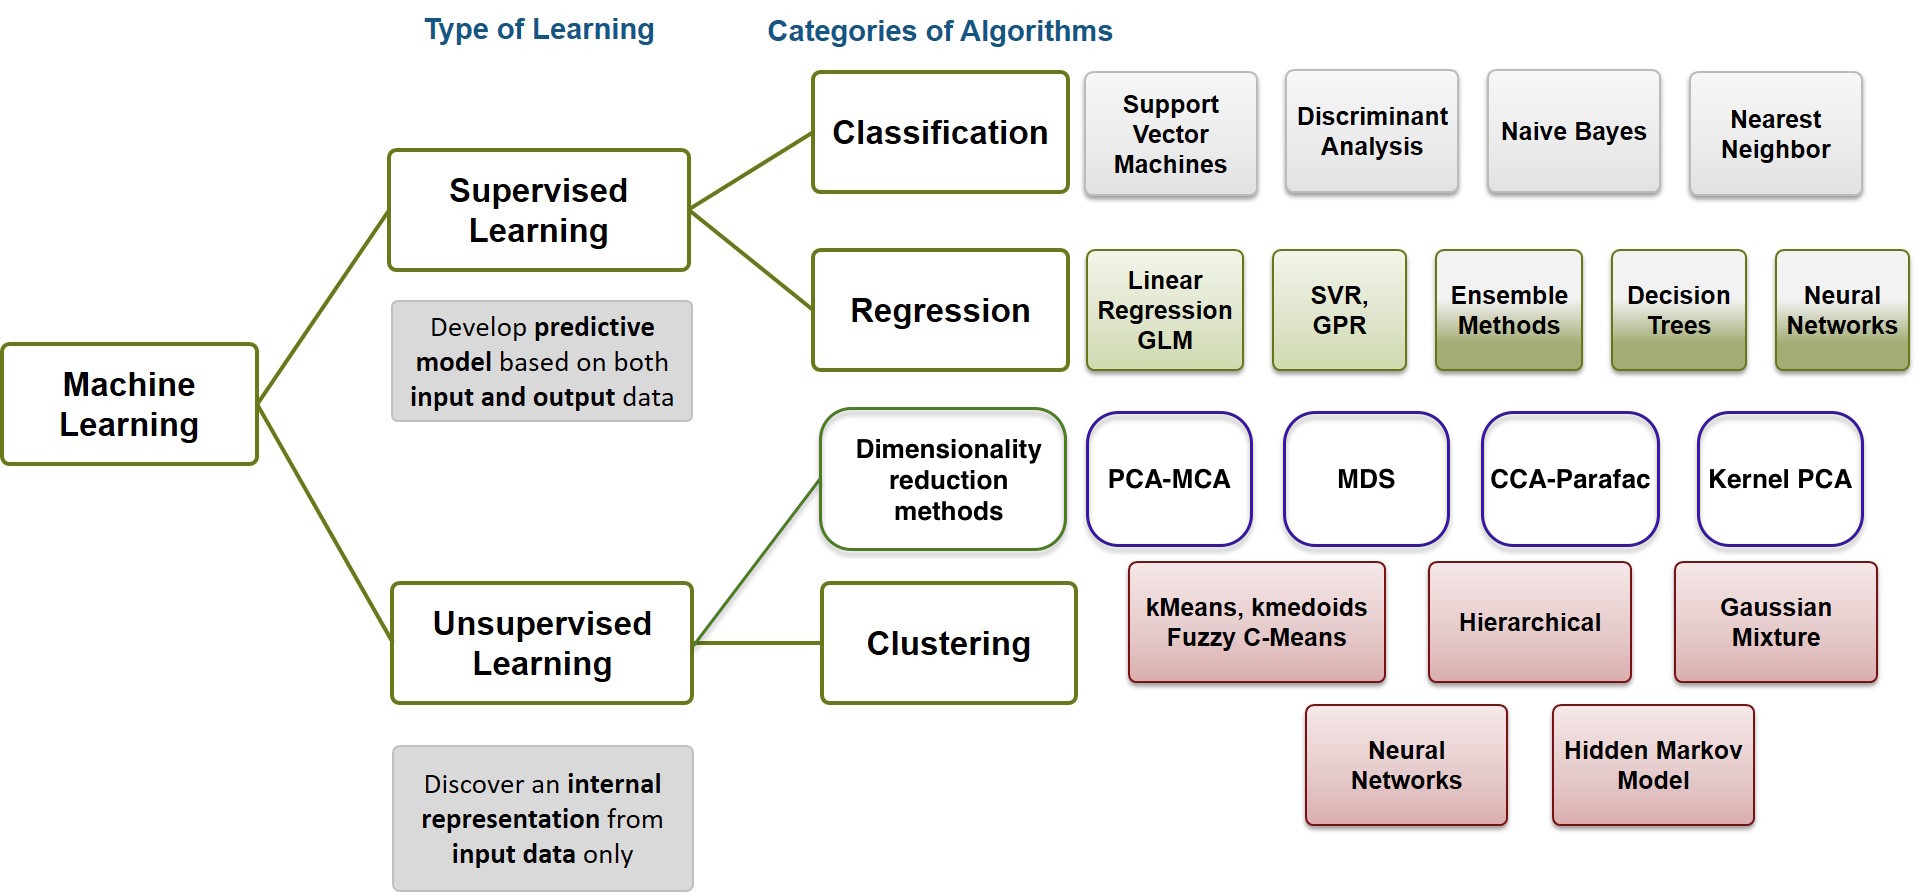
\includegraphics[width=\textwidth]{figures/Learning+Types.jpg}
	\end{center}

\end{frame}

\begin{frame}[fragile]
  \frametitle{An example in genetics: 'snp'}
  \framesubtitle{Genetics variant in European population}

\begin{block}{Description: \textcolor{black}{\it medium/large data, high-dimensional}}
500, 000 Genetics variants (SNP -- Single Nucleotide Polymorphism) for  3000 individuals
(1 meter $\times$ 166 meter (height $\times$ width)
\end{block}

\begin{multicols}{2}
  \begin{itemize}
  \item SNP : 90 \% of human genetic variations
  \item coded as 0, 1 or 2 (10, 1 or 2 allel different against the population reference)
  \end{itemize}

  \begin{figure}
    \centering
     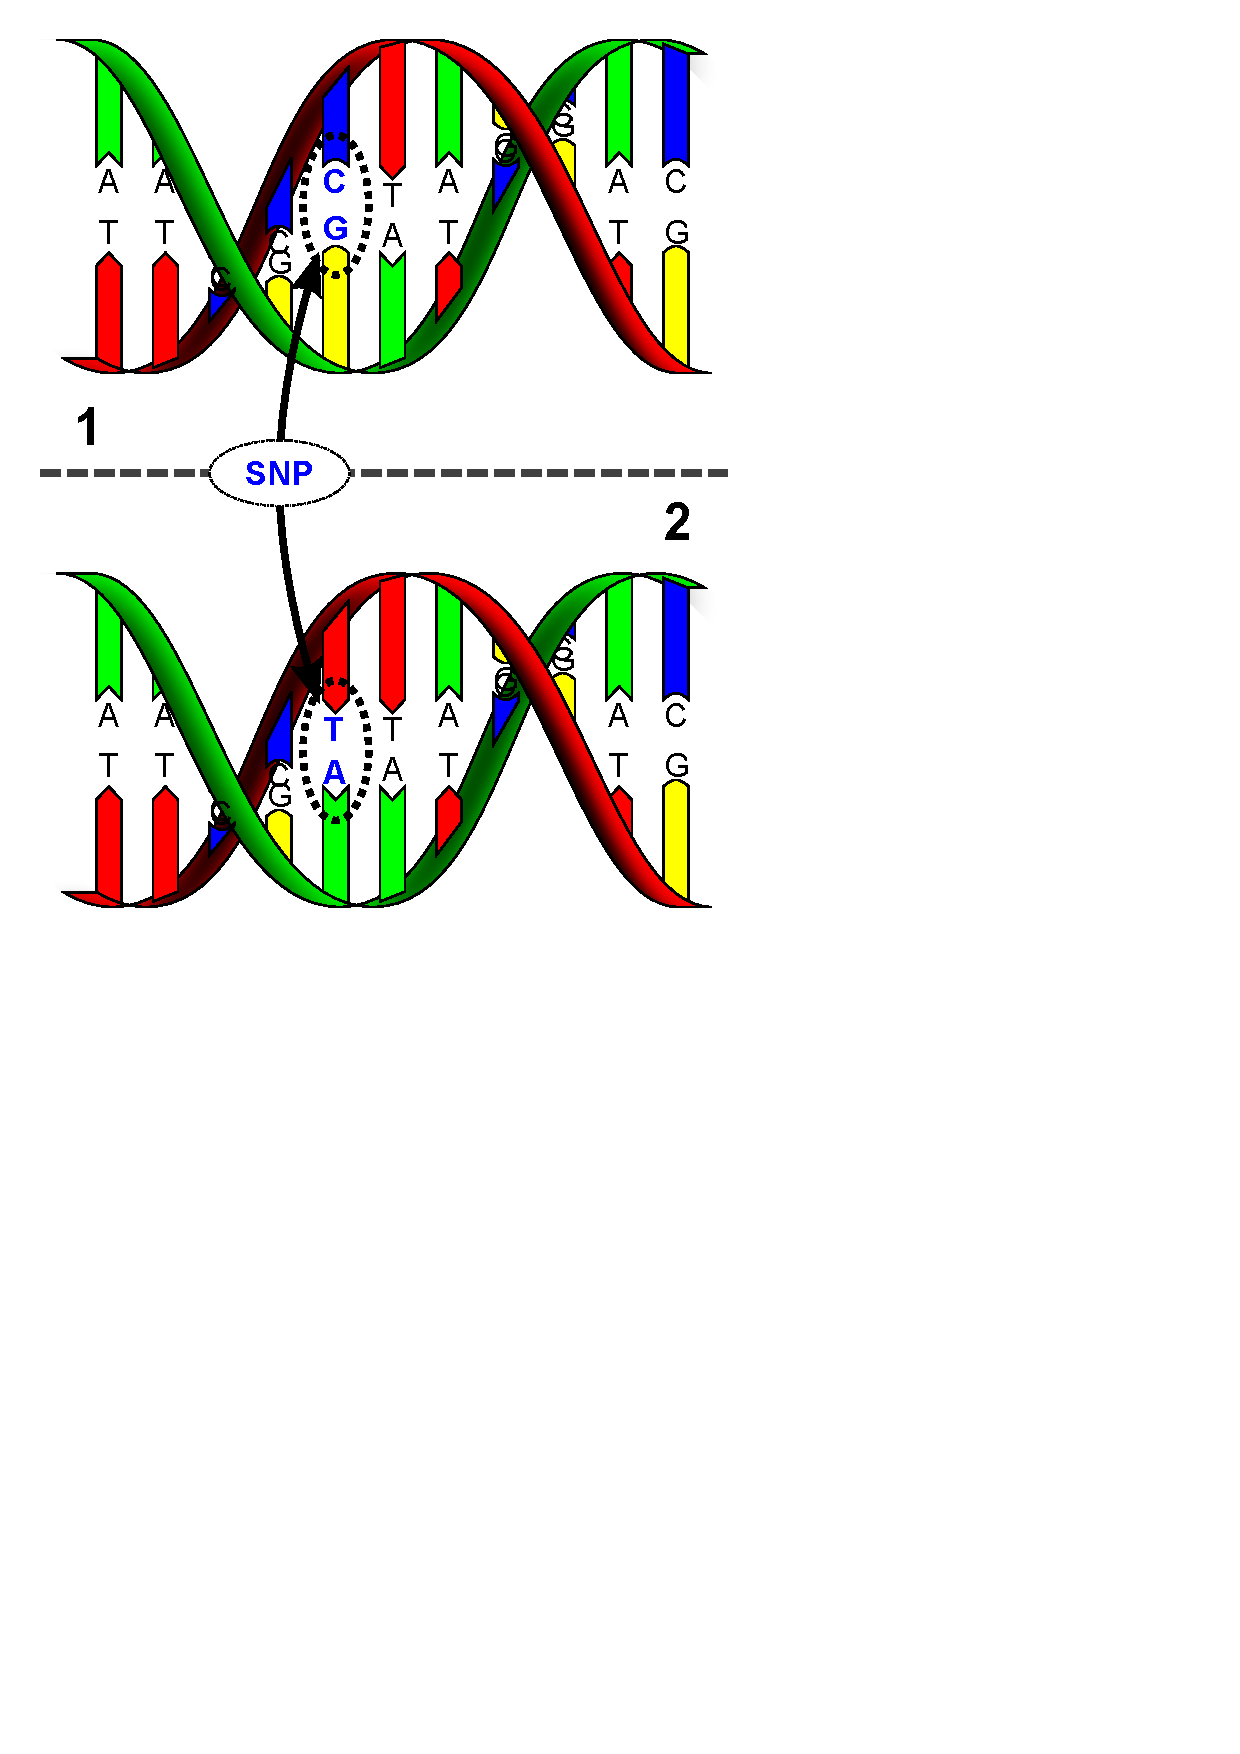
\includegraphics[height=4cm]{SNP}   
    \caption{SNP (wikipedia)}
  \end{figure}
\end{multicols}

\end{frame}


\begin{frame}
  \frametitle{Summarize 500,000 variables with 2 features}

  \begin{figure}
    \centering
      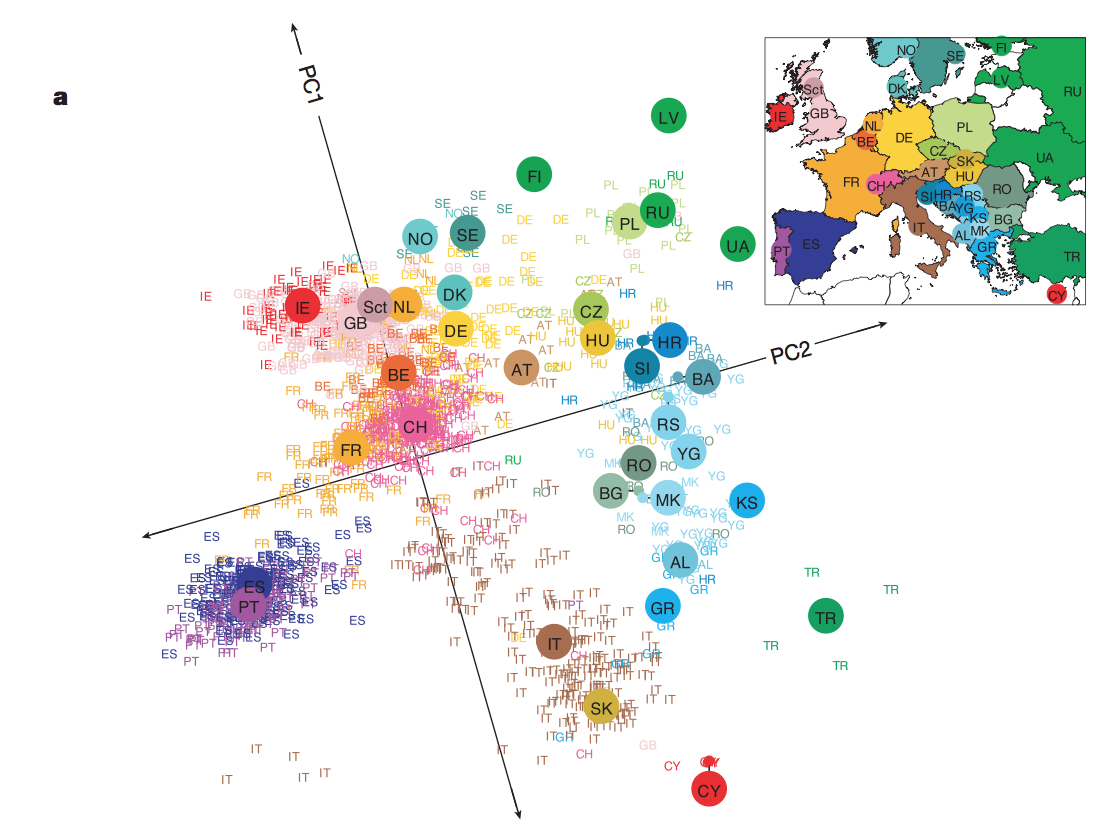
\includegraphics[height=5.5cm]{geneMirrorGeography}
    \caption{Dimension reduction + labels {\tiny source: Nature "Gene  Mirror Geography Within  Europe", 2008}}
  \end{figure}

  In the original messy $3,000 \times 500,000$ table, we may find
  \begin{itemize}
    \item an extremely strong structure between individuals (\alert{\bf "clustering"})
    \item a very simple subspace where it is obvious (\alert{\bf "dimension reduction"})
  \end{itemize}

\end{frame}

\begin{frame}[label=DimensionReduction]
  \frametitle{Dimension reduction: general goals}

  \paragraph{Main objective:} find a \alert{\bf low-dimensional representation} that captures the "essence" of (high-dimensional) data

  \vfill

  \begin{block}{Application in Machine Learning}
  \alert{Preprocessing, Regularization}
  \begin{itemize}
    \item Compression, denoising,  anomaly detection
    \item Reduce overfitting in supervised learning
  \end{itemize}
  \end{block}

\vfill

  \begin{block}{Application in Statistics/Data analysis}
    \alert{Better understanding of the data}
    \begin{itemize}
      \item descriptive/exploratory methods
      \item visualization (difficult to plot and interpret $> 3D$!)
    \end{itemize}
  \end{block}

\end{frame}

\begin{frame}
  \frametitle{Dimension reduction: problem setup}

    \begin{block}{Settings}
      \begin{itemize}
        \item \alert{Training data} : $\mathcal{D}=\{\bx_1,\ldots,\bx_n\} \in \Rset^p$,   (i.i.d.)
        \item Space $\Rset^p$ of possibly high dimension $(n \ll p)$
      \end{itemize}
    \end{block}

    \vfill
    
    \begin{block}{Dimension Reduction Map}
       Construct a map $\Phi$ from the space $\Rset^{p}$ into a space $\Rset^{q}$ of \alert{smaller dimension}:
      \begin{align*}
          \Phi:\quad & \Rset^p \to \Rset^{q}, q \ll p\\
                     & \bx \mapsto \Phi(\bx)
      \end{align*}
    \end{block}
    
\end{frame}
 
\begin{frame}
  \frametitle{How should we design/construct $\Phi$?}

  \paragraph{Criterion}
  \begin{itemize}
    \item Geometrical approach
    \item Reconstruction error
    \item Relationship preservation
  \end{itemize}

  \vfill
  
  \paragraph{Form of the map $\Phi$}
  \begin{itemize}
    \item Linear or non-linear ?
    \item tradeoff between interpretability and versatility ?
    \item tradeoff between high or low computational resource
  \end{itemize}

\end{frame}
 
% \begin{frame}
% \frametitle{Dimension Reduction?}
% 
% \begin{figure}
%   \includegraphics<1>[height=.5\textheight]{belardi-camel-3d-4}
%   \includegraphics<2>[height=.5\textheight]{belardi-camel-3d-3}
%   \includegraphics<3>[height=.5\textheight]{belardi-camel-3d-2}
%   \caption{\tiny source: F. Belardi}
% \end{figure}
% 
% \begin{itemize}
% \item How to view a high-dimensional dataset ?
% \item High-dimension: dimension larger than 2!
% \item \emph{Projection} in a 2D space.
% \end{itemize}
% \end{frame}


\begin{frame}[fragile]
  \frametitle{Companion data set: 'scRNA'}
  \framesubtitle{Subsamples of normalized Single-Cell RNAseq}

\begin{block}{Description: \textcolor{black}{\it subsample of a large data set}}
\small Gene-level expression of 100 representative genes for a collection of 301 cells 
spreaded in 11 cell-lines. Original transcription data are measured by counts obtained by 
\textit{RNAseq} and normalized to be close to a Gaussian distribution.\\

\begin{scriptsize}
\begin{thebibliography}{9}
\bibitem{pollen} Pollen, Alex A., et al. \textcolor{black}{Low-coverage single-cell mRNA sequencing reveals cellular heterogeneity and activated signaling pathways in developing cerebral cortex.} \newblock Nature biotechnology 32.10 (2014): 1053.
\end{thebibliography}
\end{scriptsize}
\end{block}

\begin{figure}
  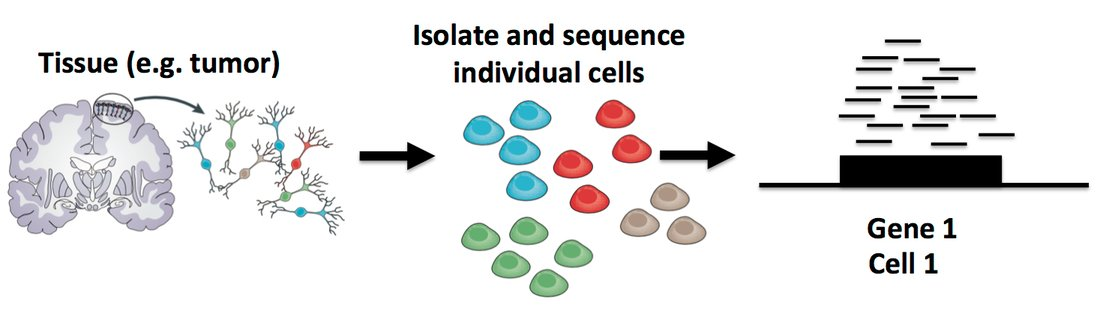
\includegraphics[width=.9\textwidth]{figures/scRNA-overview}
  \caption{Single Cell RNA sequencing data: general principle -- {\tiny source: Stephanie Hicks}}
\end{figure}

\end{frame}

\begin{frame}[fragile]
  \frametitle{Companion data set: 'scRNA'}
  \framesubtitle{Brief data summary I}

\begin{knitrout}\scriptsize
\definecolor{shadecolor}{rgb}{0.969, 0.969, 0.969}\color{fgcolor}\begin{kframe}
\begin{alltt}
\hlkwd{load}\hlstd{(}\hlstr{"../../data/scRNA.RData"}\hlstd{)}
\hlstd{scRNA} \hlkwb{<-} \hlkwd{as_tibble}\hlstd{(}\hlkwd{t}\hlstd{(pollen}\hlopt{$}\hlstd{data))} \hlopt \hlkwd{add_column}\hlstd{(}\hlkwc{cell_type} \hlstd{= pollen}\hlopt{$}\hlstd{celltypes)}
\end{alltt}
\end{kframe}
\end{knitrout}

\paragraph{Data table}
\begin{knitrout}\scriptsize
\definecolor{shadecolor}{rgb}{0.969, 0.969, 0.969}\color{fgcolor}\begin{kframe}
\begin{alltt}
\hlstd{scRNA[,} \hlnum{1}\hlopt{:}\hlnum{6}\hlstd{]} \hlopt \hlkwd{head}\hlstd{(}\hlnum{3}\hlstd{)} \hlopt \hlstd{knitr}\hlopt{::}\hlkwd{kable}\hlstd{(}\hlstr{"latex"}\hlstd{)}
\end{alltt}
\end{kframe}
\begin{tabular}{r|r|r|r|r|r}
\hline
Spike1 & MT2A & HBG2 & PRG2 & IFITM1 & ANXA1\\
\hline
0 & 12.21149 & 0 & 0 & 11.96908 & 11.837198\\
\hline
0 & 11.30622 & 0 & 0 & 12.67121 & 8.098769\\
\hline
0 & 11.92623 & 0 & 0 & 12.35984 & 10.688626\\
\hline
\end{tabular}

\end{knitrout}

\paragraph{Cell types}

\begin{knitrout}\scriptsize
\definecolor{shadecolor}{rgb}{0.969, 0.969, 0.969}\color{fgcolor}\begin{kframe}
\begin{alltt}
\hlstd{scRNA} \hlopt \hlstd{dplyr}\hlopt{::}\hlkwd{select}\hlstd{(cell_type)} \hlopt \hlkwd{summary}\hlstd{()}  \hlopt \hlstd{knitr}\hlopt{::}\hlkwd{kable}\hlstd{()}
\end{alltt}
\end{kframe}
\begin{tabular}{l|l}
\hline
  &   cell\_type\\
\hline
 & HL60   :54\\
\hline
 & K562   :42\\
\hline
 & Kera   :40\\
\hline
 & BJ     :37\\
\hline
 & GW16   :26\\
\hline
 & hiPSC  :24\\
\hline
 & (Other):78\\
\hline
\end{tabular}

\end{knitrout}

\end{frame}

\begin{frame}[fragile]
  \frametitle{Companion data set: 'scRNA'}
  \framesubtitle{Brief data summary II}

\paragraph{Histogram of normalized expression}

\begin{knitrout}\scriptsize
\definecolor{shadecolor}{rgb}{0.969, 0.969, 0.969}\color{fgcolor}\begin{kframe}
\begin{alltt}
\hlstd{scRNA} \hlopt \hlstd{dplyr}\hlopt{::}\hlkwd{select}\hlstd{(}\hlopt{-}\hlstd{cell_type)} \hlopt \hlkwd{pivot_longer}\hlstd{(}\hlkwd{everything}\hlstd{())} \hlopt
  \hlkwd{ggplot}\hlstd{()} \hlopt{+} \hlkwd{aes}\hlstd{(}\hlkwc{x} \hlstd{= value,} \hlkwc{fill} \hlstd{= name)} \hlopt{+} \hlkwd{geom_histogram}\hlstd{(}\hlkwc{show.legend} \hlstd{=} \hlnum{FALSE}\hlstd{)}
\end{alltt}
\end{kframe}
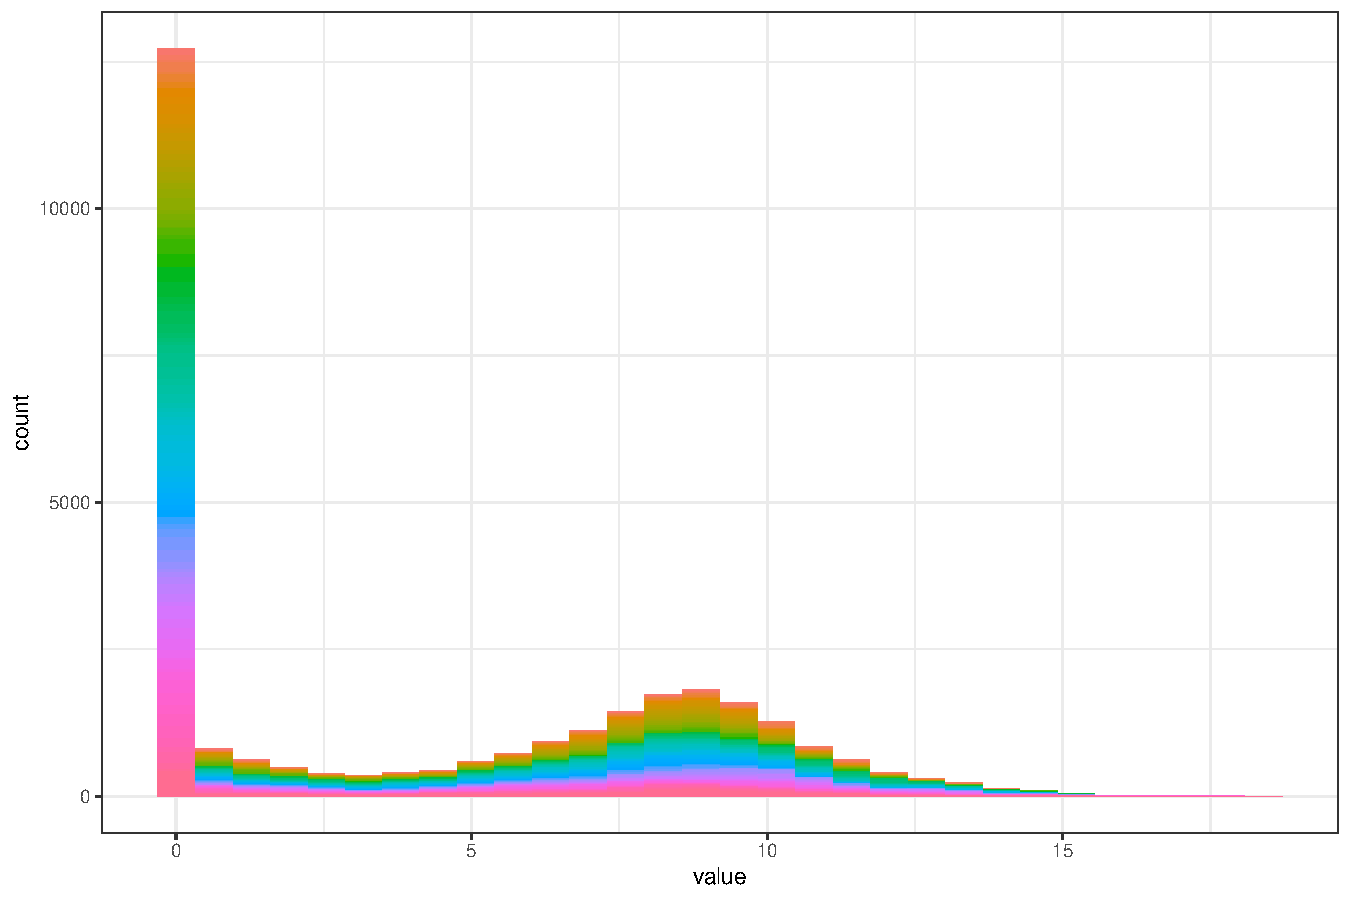
\includegraphics[width=.8\textwidth]{figures/scRNA_expressions-1} 
\end{knitrout}
\end{frame}

\begin{frame}[fragile]
  \frametitle{Companion data set: 'scRNA'}
  \framesubtitle{Brief data summary III}

\paragraph{Correlation between gene expression}

\begin{knitrout}\scriptsize
\definecolor{shadecolor}{rgb}{0.969, 0.969, 0.969}\color{fgcolor}\begin{kframe}
\begin{alltt}
\hlstd{scRNA} \hlopt \hlstd{dplyr}\hlopt{::}\hlkwd{select}\hlstd{(}\hlopt{-}\hlstd{cell_type)} \hlopt \hlkwd{cor}\hlstd{()} \hlopt
  \hlkwd{corrplot}\hlstd{(}\hlkwc{method} \hlstd{=} \hlstr{"color"}\hlstd{,} \hlkwc{tl.pos} \hlstd{=} \hlstr{"n"}\hlstd{,} \hlkwc{order} \hlstd{=} \hlstr{"hclust"}\hlstd{)}
\end{alltt}
\end{kframe}
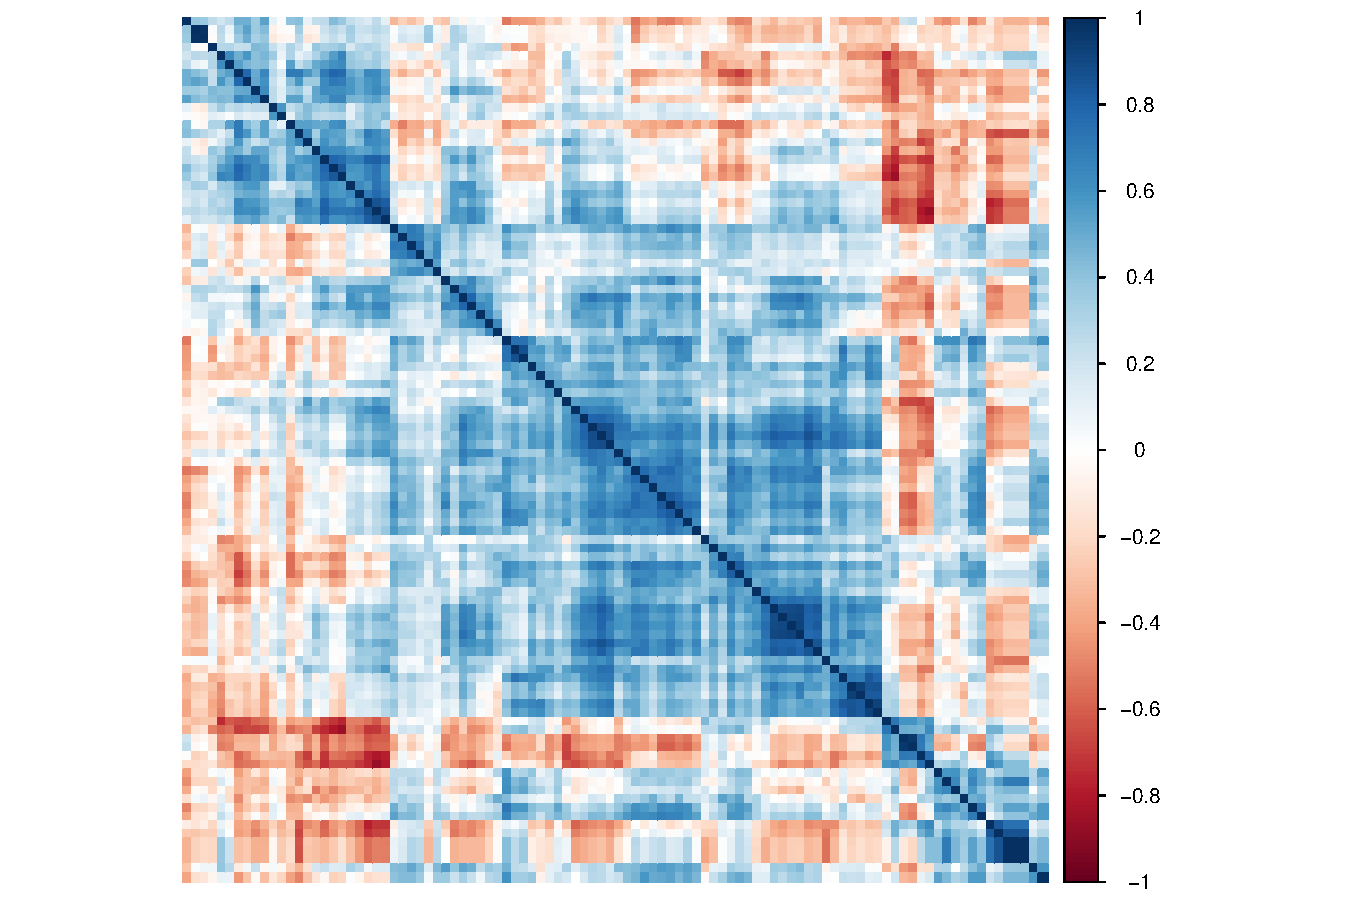
\includegraphics[width=.8\textwidth]{figures/scRNA-correlation-1} 
\end{knitrout}
\end{frame}

% \begin{frame}
% \frametitle{Theoretical argument: dimensionality Curse}
% 
% \begin{block}{High Dimension Geometry Curse}
% \begin{itemize}
% \item Folks theorem: In high dimension, everyone is alone.
% \item Theorem: If $\bx_1,\ldots, \bx_n$ in the hypercube of dimension $p$  such that their coordinates are i.i.d then
% \begin{align*}
% \mspace{-20mu} p^{-1/2} \left( \max \|\bx_i-\bx_{i'}\|_2 - \min \|\bx_i-\bx_{i'}\|_2 \right)  &= 0 + O\left(\sqrt{\frac{\log n}{p}}\right)\\
% \frac{\max \|\bx_i-\bx_{i'}\|_2}{\min \|\bx_i-\bx_{i'}\|_2} &= 1 + O\left(\sqrt{\frac{\log n}{p}}\right).
% \end{align*}
% \end{itemize}
% \end{block}
% 
%   $\rightsquigarrow$ When $p$ is large, all the points are almost equidistant\\
% 
%   Hopefully, the data \alert{\bf are not really leaving in $p$} dimension (think of the SNP example)
% 
% \end{frame}

%% ====================================================================
\part{Linear Methods}
%% ====================================================================
\begin{frame}[fragile]
  \partpage

\paragraph{Packages used to perform PCA}

\begin{knitrout}\scriptsize
\definecolor{shadecolor}{rgb}{0.969, 0.969, 0.969}\color{fgcolor}\begin{kframe}
\begin{alltt}
\hlkwd{library}\hlstd{(FactoMineR)} \hlcom{# PCA and oter linear method for dimension reduction}
\hlkwd{library}\hlstd{(factoextra)} \hlcom{# fancy plotting for FactoMineR output}
\end{alltt}
\end{kframe}
\end{knitrout}


\end{frame}


\begin{frame}
  \frametitle{PCA and classical Linear methods}
  
  \paragraph{\bf Principal component Analysis (PCA) is for continuous data}

  \begin{block}{Non continuous data}
  \begin{itemize}
    \item Correspondence analysis (CA): contingency table \medskip
    \item Multiple correspondence analysis (MCA): categorical data \medskip
    \item Multiple factor analysis (MFA): multi-table, array data 
  \end{itemize}
  $\rightsquigarrow$ Basic \alert{adaptations that build on PCA} to deal with non-continuous data\\
  $\rightsquigarrow$ smart encoding of non-continuous data to continuous ones
  \end{block}

  \vfill
  
  \begin{center}
    \alert{\bf We will focus on PCA}, as the mother of most linear (and non-linear) methods.
  \end{center}
  
\end{frame}

\begin{frame}
  \frametitle{Objectives}
  
\paragraph{Individual/Observations}
  
  \begin{itemize}
    \item similarity between observations with respect to all the variables 
    \item Find pattern ($\sim$ partition) between individuals
  \end{itemize}

\vfill

\paragraph{Variables} 
  
  \begin{itemize}
  \item linear relationships between variables 
  \item find synthetic variables
  \end{itemize}

\vfill

\paragraph{Link between the two}
  
  \begin{itemize}
    \item characterization of the groups of individuals with variables
    \item specific observations to understand links between variables
  \end{itemize}

\end{frame}

%% ==========================================================================
%% Background: high-school algebra
%% ==========================================================================
%% ==========================================================================
\section{Background: high-school algebra}
%% ==========================================================================

\begin{frame}
  \frametitle{Vectors in $\Rset^n$}
  \framesubtitle{Definition and Basics}

   A vector $\bx\in\Rset^d$ is defined by a $d$-uplet $(x_1, x_2, \dots, x_d)$, \textit{its coordinates}.

  \begin{block}{Elementary operations}
  \vspace{-.5cm}
  \begin{multicols}{2}
   \begin{itemize}
    \item Addition of two vectors (define a parallelogram)
    \begin{equation*}
    \bx + \by = \begin{pmatrix}
    x_1 + y_1 \\ x_2 + y_2 \\ \vdots \\ x_d + y_d
    \end{pmatrix}
  \end{equation*}
    \item Multiplication by a scalar (streching)
   \end{itemize}
  \begin{equation*}
    \lambda \bx = \begin{pmatrix}
    \lambda x_1 \\ \lambda x_2 + c \\ \vdots \\ \lambda x_d
    \end{pmatrix}, \quad \lambda, c \in \Rset.
  \end{equation*}
  \end{multicols}
  \end{block}

  \begin{block}{Properties}
  \vspace{-.5cm}
  \begin{multicols}{2}
    \begin{itemize}
      \item associativity: $(\bx + \by) + \bz = \bx + (\by + \bz)$
      \item commutativity: $\bx + \by = \by + \bx$
      \item linearity: $\lambda (\bx + \by) = \lambda \bx + \lambda \by$
      \item $(\lambda_1 + \lambda_2) \bx = \lambda_1\bx + \lambda_2 \bx$
    \end{itemize}  
  \end{multicols}
  \end{block}
  
\end{frame}

\begin{frame}
  \frametitle{Vectors in $\Rset^n$}
  \framesubtitle{Dot/Inner product and norm}

  \begin{block}{Dot product of 2 vectors: \textcolor{black}{sum of the products between each coordinate:}}
  \vspace{-.25cm}
  \begin{equation*}
    \langle \bx, \by \rangle \equiv \bx \cdot \by \equiv \bx^\top \by \triangleq \sum_{i=1}^d x_i \, y_j.
  \end{equation*}
  \begin{multicols}{2}
  \begin{itemize}
    \item $\bx^\top \by = \by^\top \bx$
    \item $\bx^\top (\by + \bz) = \bx^\top \by + \bx^\top \bz$
    \item $\lambda (\bx^\top \by) = (\lambda (\bx)^\top \by = \bx^\top (\lambda \by) $
    \item if $\bx = \bzero$, then $\bx^\top \bx = 0$.
  \end{itemize}
  \end{multicols}
  \end{block}

  \begin{block}{(Euclidean) norm (a.k.a length, magnitude) } 
  \vspace{-.35cm}
    \begin{equation*}
      \| \bx \| = \sqrt{\bx^\top \bx}. \quad \textrm{we have }   \| \lambda \bx \| = |\lambda| \| \bx \|.
    \end{equation*}
  \end{block}

\end{frame}

\begin{frame}
  \frametitle{Vectors in $\Rset^n$}
  \framesubtitle{Distances and orthogonality}

  \begin{block}{(Euclidean) distance between 2 vectors} 
    \begin{equation*}
      \distance(\bx, \by) = \| \bx - \by \|.
    \end{equation*}
  \end{block}

  \pause
  
  Remark that when $\bx$ and $\by$ are orthogonal and non zero, distances between $\bx$ and $\by$ and $\bx$ and $(-\by)$ are the same. Then, 
  \begin{equation*}
    (\bx - \by)^\top(\bx - \by) = (\bx + \by)^\top(\bx + \by) \Leftrightarrow \bx^\top\by  = 0,
  \end{equation*}
  
  which motivates the following definition of orthornality:
  \begin{block}{Orthogonality}
  Two vectors $\bx, \by \neq \bzero$ are orthogonal iff $\bx^\top \by = 0$.
  \end{block}

\end{frame}


\begin{frame}
  \frametitle{Vectors in $\Rset^n$}
  \framesubtitle{Orthogonal Projection and geometric definition of the dot product}

  \begin{columns}
  \begin{column}{.5\textwidth}
  \begin{block}{Orthogonal projection of $\bx$ onto $\by$}
    It is the vector $\bz$ such that
  \begin{enumerate}
    \item $\bz = \lambda \by$
    \item $\by$  is orthogonal to $\bx - \bz$
  \end{enumerate}
    We find $\lambda =\bx^\top \by / \|\by \|^2 $ 
  \end{block}
  \end{column}
  \begin{column}{.5\textwidth}
    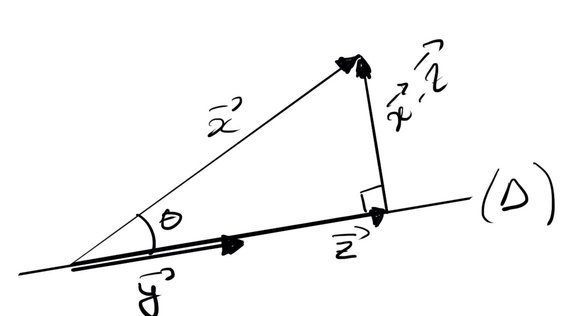
\includegraphics[width=\textwidth]{scalar_projection}
  \end{column}
  \end{columns}

  \pause
  Thanks to Pythagoras theorem, 
  \begin{equation*}
    \cos(\theta) = \frac{\|\bz\|}{\|\bx\|} = \lambda \frac{\|\by\|}{\|\bx\|}
  \end{equation*}
  and then we end with the following geometric definition of the dot product
  
  \begin{block}{Dot product: geometric definition} 
  \vspace{-.35cm}
    \begin{equation*}
      \bx^\top \by = \cos (\theta) \| \bx \| \,  \| \by \| 
    \end{equation*}
  \end{block}


\end{frame}


%% ==========================================================================
%% Geometric point of View
%% ==========================================================================

%% ==========================================================================
\section{Geometric approach to PCA}
%% ==========================================================================

\begin{frame}[fragile]
  \frametitle{The data matrix}

  The data set is a $n\times p$ matrix  $\bX = (x_{ij})$ with values in $\Rset$:
  \begin{itemize}
    \item each row $\bx_i$ represents an individual/observation
    \item each col $\bx^j$ represents a variable/attribute
  \end{itemize}

  \begin{equation*}
    \bX = \bordermatrix{%
           ~ & \bx^1  & \bx^2  &  \dots & \bx^j   & \dots & \bx^p  \cr
    \bx_1  & x_{11} & x_{12} &  \dots & x_{1j} & \dots & x_{1p}  \cr
    \bx_2  & x_{21} & x_{22} &  \dots & x_{2j} & \dots & x_{2p}  \cr
    \vdots & \vdots & \vdots & \vdots & \vdots & \vdots & \vdots  \cr
    \bx_i  & x_{i1} & x_{i2} &  \dots & x_{ij} & \dots & x_{ip} \cr
    \vdots & \vdots & \vdots & \vdots & \vdots & \vdots & \vdots  \cr
    \bx_n  & x_{n1} & x_{n2} &  \dots & x_{nj} & \dots & x_{np} \cr
    }
  \end{equation*}

\begin{knitrout}\scriptsize
\definecolor{shadecolor}{rgb}{0.969, 0.969, 0.969}\color{fgcolor}\begin{kframe}
\begin{alltt}
\hlstd{scRNA[,} \hlnum{1}\hlopt{:}\hlnum{8}\hlstd{]} \hlopt \hlkwd{head}\hlstd{(}\hlnum{3}\hlstd{)} \hlopt \hlstd{knitr}\hlopt{::}\hlkwd{kable}\hlstd{(}\hlstr{"latex"}\hlstd{)}
\end{alltt}
\end{kframe}
\begin{tabular}{r|r|r|r|r|r|r|r}
\hline
Spike1 & MT2A & HBG2 & PRG2 & IFITM1 & ANXA1 & HBG1 & MPO\\
\hline
0 & 12.21149 & 0 & 0 & 11.96908 & 11.837198 & 0 & 0\\
\hline
0 & 11.30622 & 0 & 0 & 12.67121 & 8.098769 & 0 & 0\\
\hline
0 & 11.92623 & 0 & 0 & 12.35984 & 10.688626 & 0 & 0\\
\hline
\end{tabular}

\end{knitrout}

\end{frame}

\begin{frame}
  \frametitle{Cloud of observation in $\Rset^p$}

  Individuals can be represented in the \alert{variable space $\Rset^p$} as a point cloud

  \begin{columns}
    \begin{column}{.5\textwidth}
      \begin{figure}      
      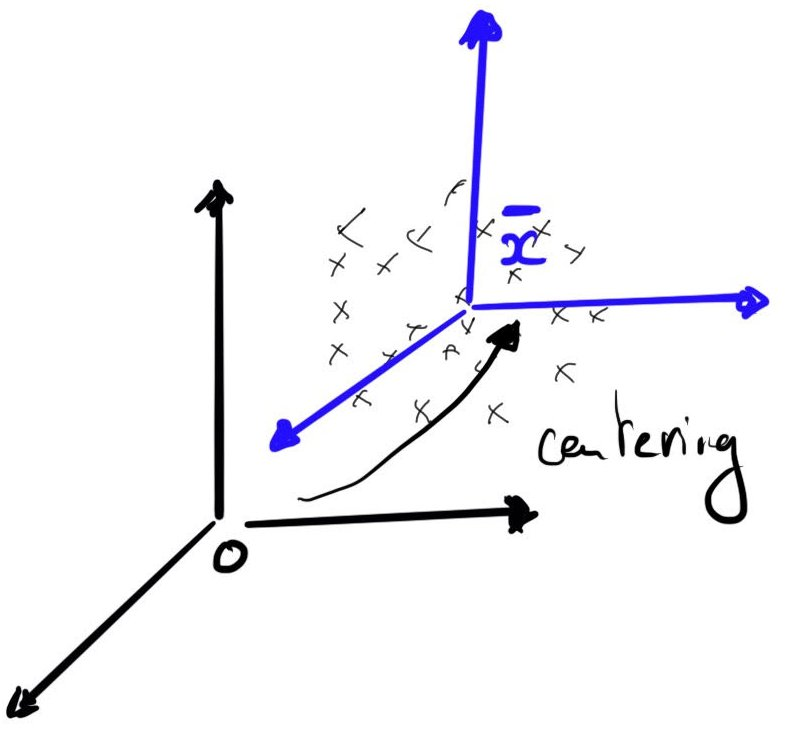
\includegraphics[width=.6\textwidth]{cloud_centering}
      \vspace{-.25cm}
      \caption{Example in $\Rset^3$}
      \end{figure}      
    \end{column}

  \begin{column}{.5\textwidth}
    \begin{block}{Center of Inertia}
      (or barycentrum, or empirical mean)
      \[ \bar{\bx} = \frac{1}{n} \sum _{i=1}^n \bx_i = 
      \begin{pmatrix}
        \sum _{i=1}^n x_{i1}/n \\
        \sum _{i=1}^n x_{i2}/n \\
        \vdots\\
        \sum _{i=1}^n x_{ip}/n
      \end{pmatrix}
      \]
    \end{block}
  \end{column}
  \end{columns}

  We center the cloud $\bX$ around $\bx$ denote this by $\bX^c$
  \begin{equation*}
    \bX^c = \begin{pmatrix}
    x_{11} - \bar{x}_1 &   \dots & x_{1j}  - \bar{x}_j & \dots  & x_{1p} - \bar{x}_p   \cr
              \vdots   &  \vdots & \vdots              & \vdots & \vdots  \cr
    x_{i1} - \bar{x}_1 &   \dots & x_{ij} - \bar{x}_j  & \dots  & x_{ip}  - \bar{x}_p \cr
              \vdots   &  \vdots & \vdots              & \vdots & \vdots  \cr
    x_{n1} - \bar{x}_1 &  \dots  & x_{nj} - \bar{x}_j  & \dots  & x_{np}  - \bar{x}_p \cr
    \end{pmatrix}
  \end{equation*}

\end{frame}

\begin{frame}
  \frametitle{Inertia and Variance}

\begin{block}{Total Inertia: \textcolor{black}{distance of the individuals to the center of the cloud}}
  \[
      I_T = \frac{1}{n}\sum_{i=1}^n \sum_{j=1}^p  (x_{ij}- \bar{x}_{j}) ^2 
      = \frac{1}{n}\sum_{i=1}^n \|\bx_i - \bar{\bx} \|^2  
      = \frac{1}{n}\sum_{i=1}^n \distance^2 (\bx_i,\bar{\bx})
    \]
\end{block}

  \begin{block}{$I_T$ is proportional to the total variance}
  Let $\hat{\bSigma}$ be the empirical variance-covariance matrix
\[
      I_T = \frac{1}{n}\sum_{j=1}^p  \sum_{i=1}^n (x_{ij}- \bar{x}_{j}) ^2 
      = \sum_{j=1}^p \frac{1}{n}\|\bx^j - \bar{x}_{j} \|^2
      = \sum_{j=1}^p \var(\bx^j) = \trace{\hat{\bSigma}}
\]
\end{block}

\begin{itemize}
  \item[$\rightsquigarrow$] \alert{Good representation has large inertia} (much variability)
  \item[$\rightsquigarrow$] \alert{Large dispertion $\sim$ Large distances between points}
\end{itemize}
  
\end{frame}

\begin{frame}
  \frametitle{Inertia with respect to an axis}

  The Inertia of the cloud wrt axe $\Delta$ is the sum of the distances between all points and their orthogonal projection on $\Delta$.
  \begin{equation*}
    \begin{aligned}
      I_\Delta = \frac{1}{n}\sum_{i=1}^n \distance^2(\bx_i, \Delta)
      \end{aligned}
  \end{equation*}

  \begin{figure}
    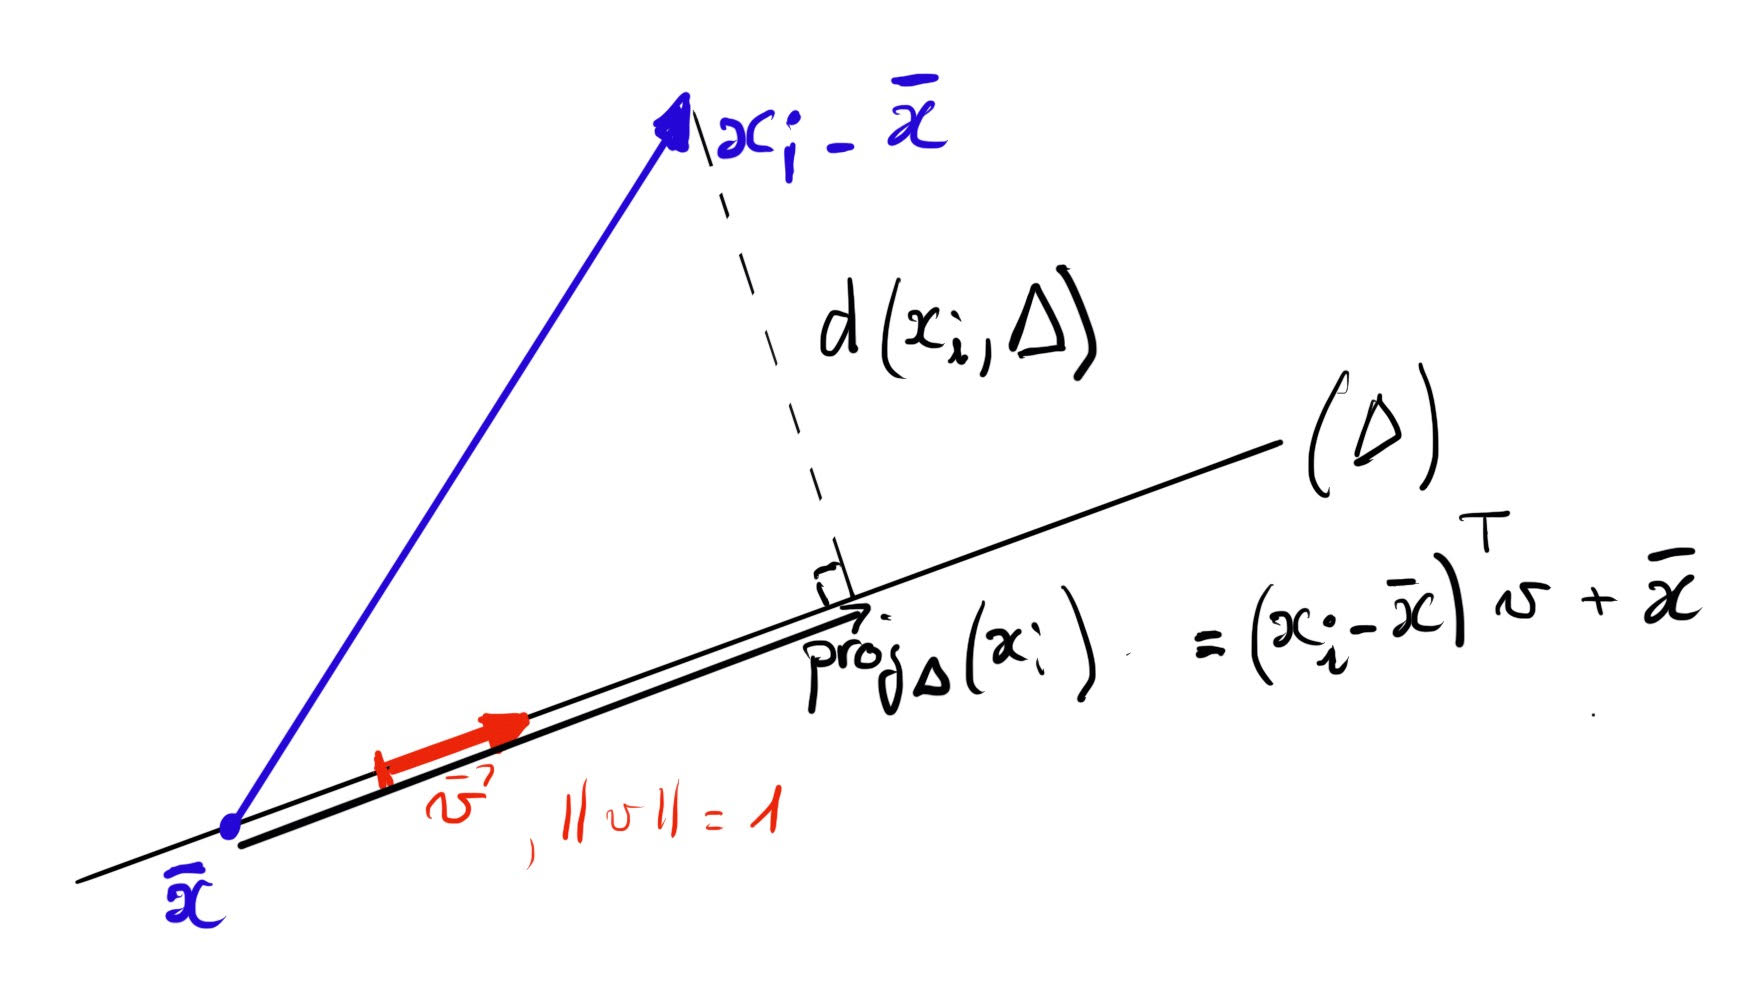
\includegraphics[width=.7\textwidth]{proj_axis}
    \caption{Projection of $\bx_i$ onto a line $\Delta$ passing through $\bar\bx$}
  \end{figure}

\end{frame}

\begin{frame}
  \frametitle{Decomposition of total Inertia (1)}
  
  Let $\Delta^\bot$ be the orthogonal subspace of $\Delta$ in $\Rset^p$

  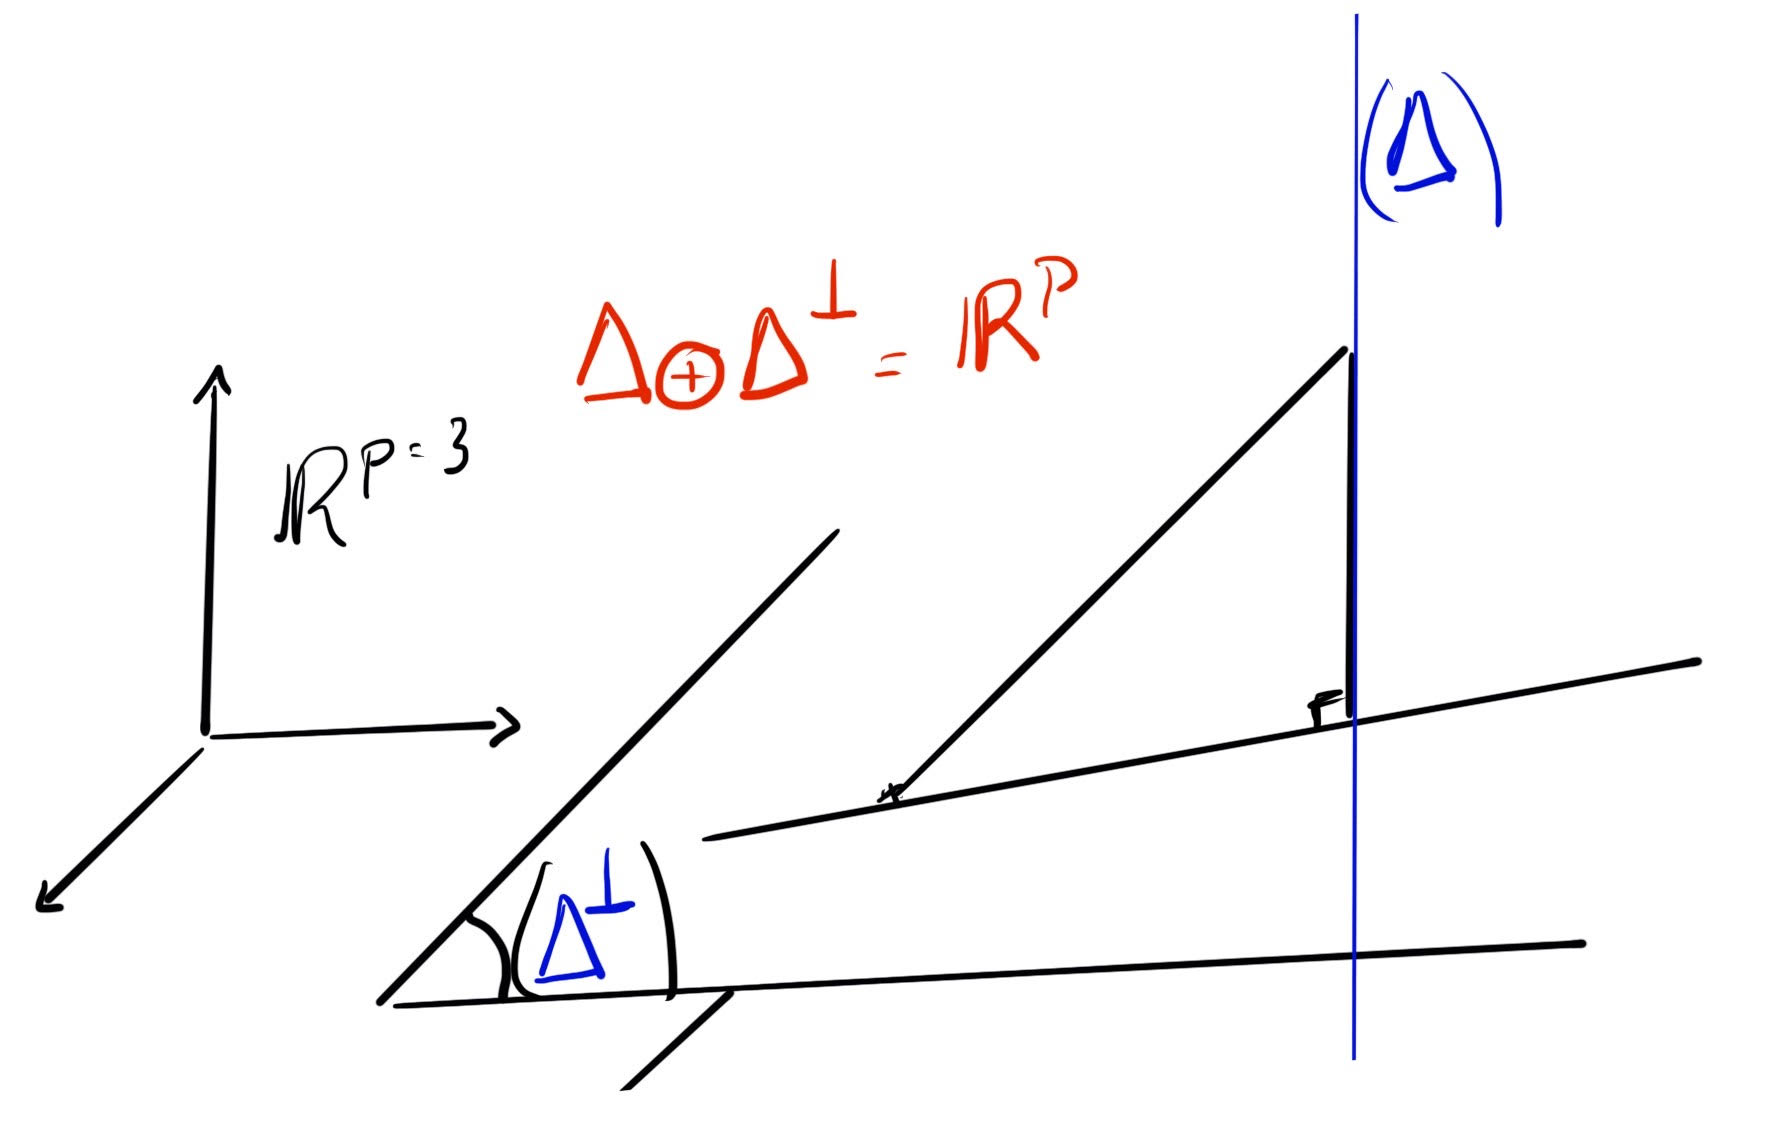
\includegraphics[width=.5\textwidth]{supp_spaces}

  \begin{block}{Theorem (Huygens)}
    A consequence of the above (Pythagoras Theorem) is the decomposition of the following total inertia:
      \begin{equation*}
        I_T = I_{\Delta} + I_{\Delta^\bot}
      \end{equation*}
    \alert{By projecting the cloud $\bX$ onto $\Delta$, with loss the inertia measured by $\Delta^\bot$}
    \end{block}
        
\end{frame}

\begin{frame}
  \frametitle{Decomposition of total Inertia (2)}
  
  Consider only subspaces with dimension $1$ (that is, lines or axes). We can decompose $\Rset^p$ as the sum of $p$ othogonal axis. 
  
  \begin{equation*}
    \Rset^p = \Delta_1 \oplus \Delta_2 \oplus \dots \oplus \Delta_p
  \end{equation*}
  \alert{$\rightsquigarrow$ These axes form a new basis for representing the point cloud.}

  \begin{block}{Theorem (Huygens)}
    \begin{equation*}
      I_{T} = I_{\Delta_1} + I_{\Delta_2} + \dots + I_{\Delta_p}
    \end{equation*}
  \end{block}
  
\end{frame}

%% ==========================================================================
%% Principal axes by variance maximization
%% ==========================================================================

%% ==========================================================================
\section{Principal axes and variance maximization}
%% ==========================================================================

\begin{frame}
  \frametitle{Finding the best axis (1)}

  \begin{block}{Definition of the problem}
    \begin{itemize}
      \item The best axis $\Delta_1$ is the "closest" to the point cloud
      \item Inertia of $\Delta_1$ measures the distance between the data and $\Delta_1$
      \item $\Delta_1$ is defined by the director vector $\bv_1$, such as $\| \bv_1 \| = 1$
      \item $\Delta_1^\bot$ is defined by the normal  vector $\bv_1$, such as $\| \bv_1 \| = 1$
    \end{itemize}
    \alert{$\rightsquigarrow$ The best axis $\Delta_1$ is the one with the minimal Inertia.}
  \end{block}
  
\end{frame}

\begin{frame}
  \frametitle{Finding the best axis (2)}

  \begin{block}{Stating the optimization problem}
    Since $\Delta_1 \oplus \Delta_1^\bot = \Rset^p$ and $I_T = I_{\Delta_1} + I_{\Delta_1^\bot}$ , then
    \begin{equation*}
        \minimize_{\bv \in \Rset^p: \|\bv\| = 1} I_{\Delta_1} \Leftrightarrow \maximize_{\bv \in \Rset^p: \|\bv\| = 1} I_{\Delta_1^\bot}
    \end{equation*} 
  \end{block}  
  
  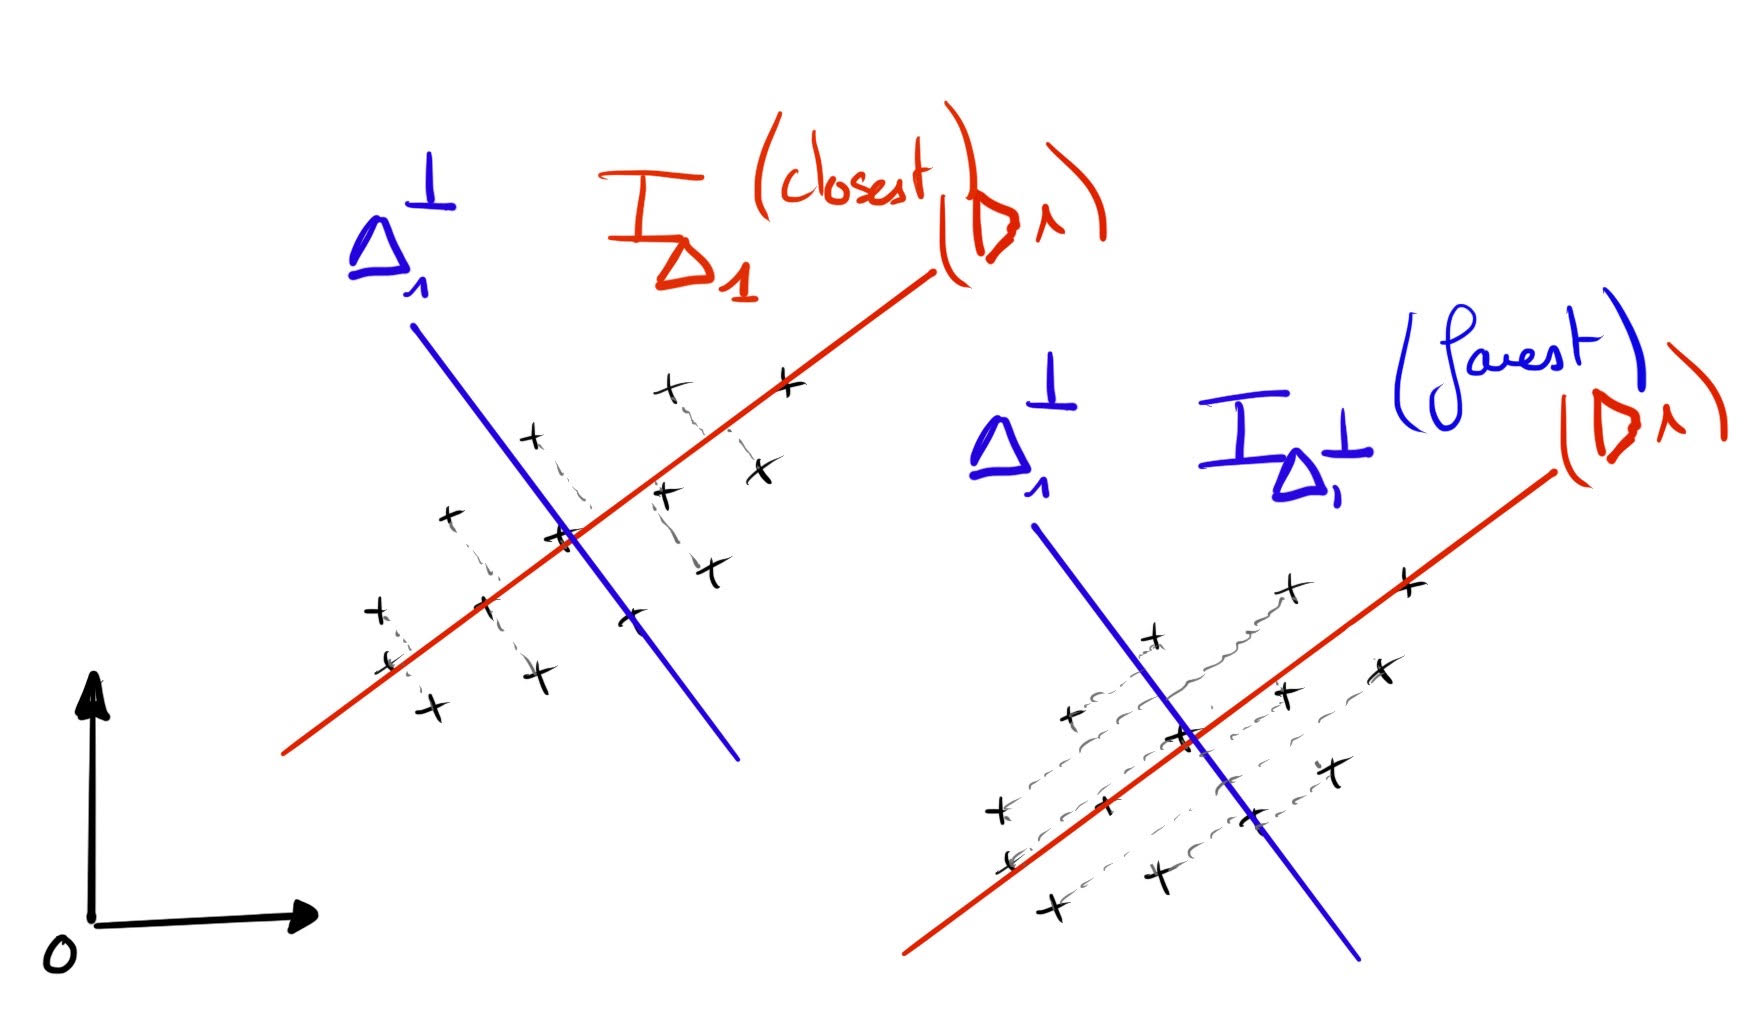
\includegraphics[width=.7\textwidth]{minimum_inertia}
  
\end{frame}

\begin{frame}
  \frametitle{Finding the best axis (3)}

\begin{columns}
  \begin{column}{.5\textwidth}
  \begin{block}{Stating the problem (algebraically)}
    Find $\bv_1; \|\bv_1 \|=1$ that maximizes
    \begin{equation*}
      \begin{aligned}
        I_{\Delta_1^\bot} & = \frac{1}{n}\sum_{i=1}^n \distance(\bx_i,\Delta_1^\bot)^2 \\ 
        & = \frac{1}{n}\sum_{i=1}^n \bv_1^\top (\bx_i - \bar{\bx})(\bx_i - \bar{\bx})^\top \bv_1 \\
        & = \bv_1^\top \left( \sum_{i=1}^n \frac{1}{n}(\bx_i - \bar{\bx})(\bx_i - \bar{\bx})^\top \right)  \bv_1 \\
        & = \bv_1^\top \hat{\bSigma}  \bv_1
      \end{aligned}
    \end{equation*} 
  \end{block}  
  \end{column}
  \begin{column}{.45\textwidth}
  \begin{figure}
    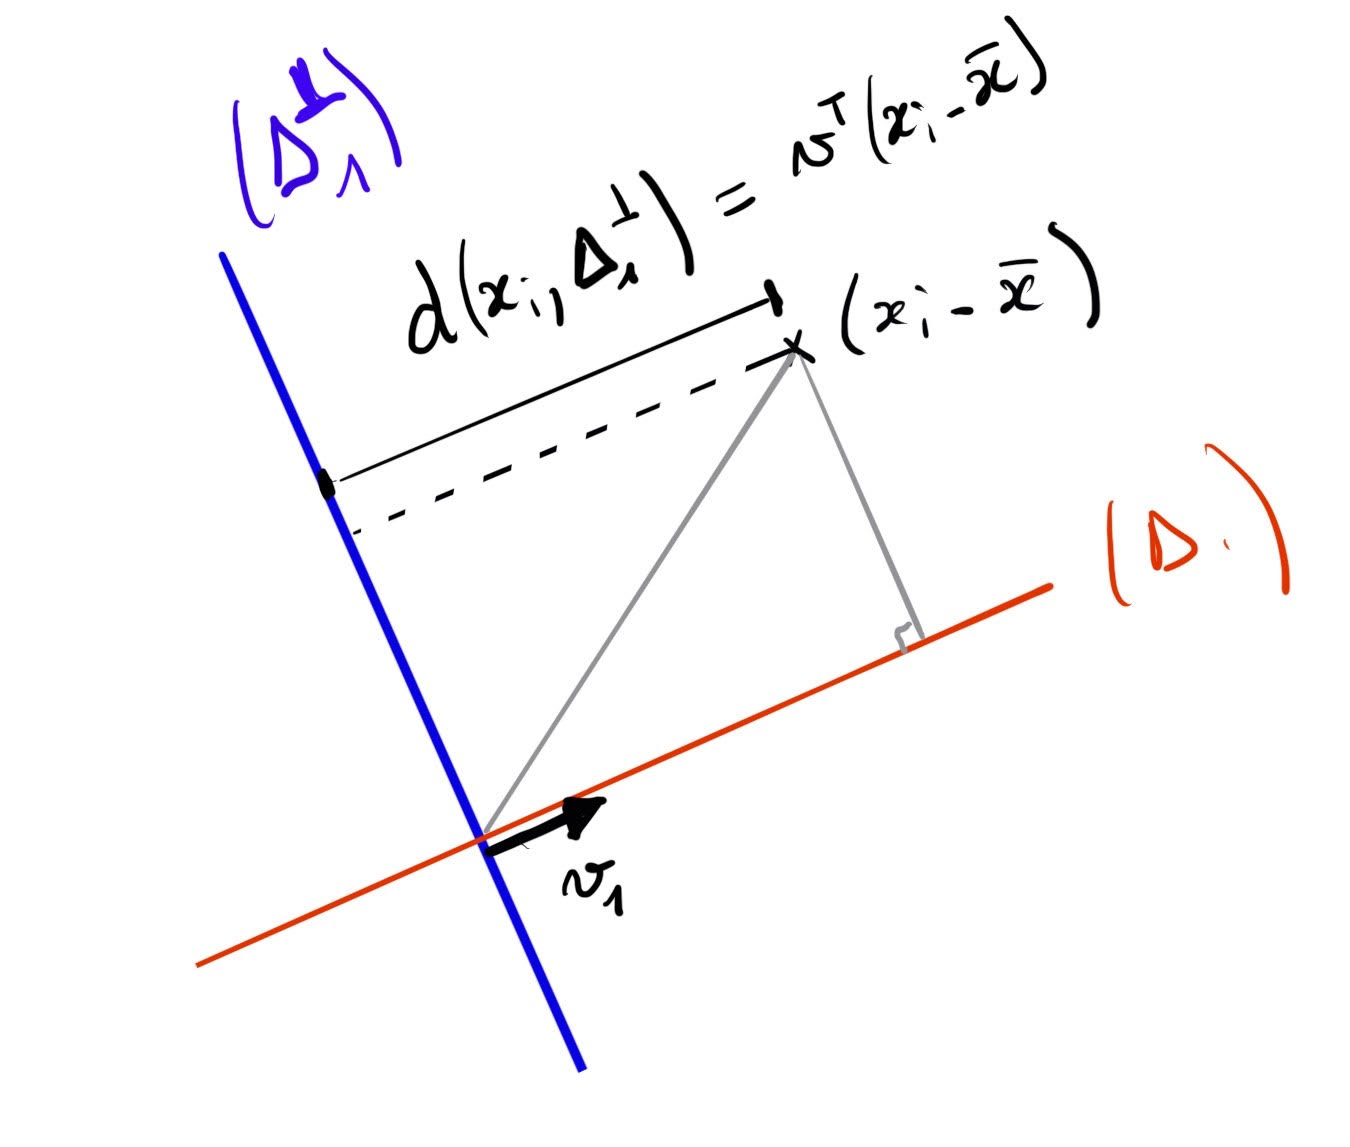
\includegraphics[width=.9\textwidth]{solving_inertia}
    \caption{Geometrical insight}
  \end{figure}
  \end{column}
\end{columns}
  
\end{frame}

\begin{frame}
  \frametitle{Finding the best axis (4)}

  We solve a simple constraint maximization problem with the method of Lagrange multipliers:
  
  \begin{equation*}
    \maximize_{\bv_1: \|\bv_1\| = 1 } \bv_1^\top \hat\bSigma \bv_1 \Leftrightarrow \maximize_{\bv_1\in\Rset^p, \lambda_1 > 0} \bv_1^\top \hat\bSigma \bv_1 - \lambda_1 (\|\bv_1\|^2 - 1)
  \end{equation*}
  
  By straightforward (vector) differentiation, an using that $\bv_1^\top \bv_1 = 1$
  \begin{equation*}
    \left\{\begin{aligned}
      2\hat\bSigma \bv_1 - 2\lambda_1 \bv_1 & = 0 \\  
      \bv_1^\top \bv_1 - 1 & = 0 \\  
    \end{aligned}\right. \Leftrightarrow
    \left\{\begin{aligned}
      \hat\bSigma \bv_1 & = \lambda_1 \bv_1  \\  
      \bv_1^\top \hat\bSigma \bv_1 & = \lambda_1 \bv_1^\top \bv_1 = \lambda_1 = I_{\Delta_1}^\bot \\  
    \end{aligned}\right.
  \end{equation*}
  
  \begin{itemize} 
     \item $\bv_1$ is the first (normalized) eigen vector of $\hat{\bSigma}$
     \item $\lambda_1$ is the first eigen value of $\hat{\bSigma}$
   \end{itemize} 
  
  $\rightsquigarrow$ \alert{\bf $\Delta_1$ is defined by the first eigen vector of $\hat\bSigma$}\\
  $\rightsquigarrow$ \alert{\bf Variance "carried" by $\Delta_1$ is equal to the largest eigen value of $\hat\bSigma$}
  
\end{frame}

\begin{frame}
  \frametitle{Finding the following axes}

  \begin{block}{Second best axis}
    Find $\Delta_2$ with dimension 1, director vector $\bv_2$ orthogonal to $\Delta_1$ solving
    \begin{equation*}
        \maximize_{\bv_2 \in \Rset^p} I_{\Delta_2^\bot} = \bv_2^\top \hat{\bSigma}\bv_2, \quad \text{with } \|\bv_2\| = 1, \bv_1^\top \bv_2 = 0.
    \end{equation*} 
  $\rightsquigarrow$ $\bv_2$ is the second eigen vector of $\hat\bSigma$ with eigen value $\lambda_2$
  \end{block}
  
  \vfill
  \pause
  
  \begin{block}{And so on!}
    PCA is roughly a matrix factorisation problem 
    \begin{equation*}
      \hat\bSigma = \bV \boldsymbol\Lambda \bV^\top, \quad
      \bV = \begin{pmatrix}
      \bv_1 & \bv_2, & \dots & \bv_p
      \end{pmatrix}, \quad \boldsymbol\Lambda = \diag(\lambda_1, \dots, \lambda_p)
    \end{equation*}
    \hspace{-.5cm}
  \begin{itemize}
    \item $\bV$ is an orthogonal matrix of normalized eigen vectors.
    \item $\boldsymbol\Lambda$ is diagonal matrix of  ordered eigen values.
  \end{itemize}
  \end{block}
\end{frame}

\begin{frame}
  \frametitle{Interpretation in $\Rset^p$}
    
  $\bV$ describes a new orthogonal basis and a rotation of data in this basis\\
  $\rightsquigarrow$ PCA is an appropriate rotation on axes that maximizes the variance

  \begin{equation*}
    \left\{\begin{array}{ccccc}
      \Delta_1 & \oplus & \dots & \oplus & \Delta_p \\
      \bv_1 & \bot & \dots & \bot & \bv_p \\
      \lambda_1 & > & \dots & > & \lambda_p \\
      I_{\Delta_1^\bot} & > & \dots & > & I_{\Delta_p^\bot} \\
    \end{array}\right.
  \end{equation*}

  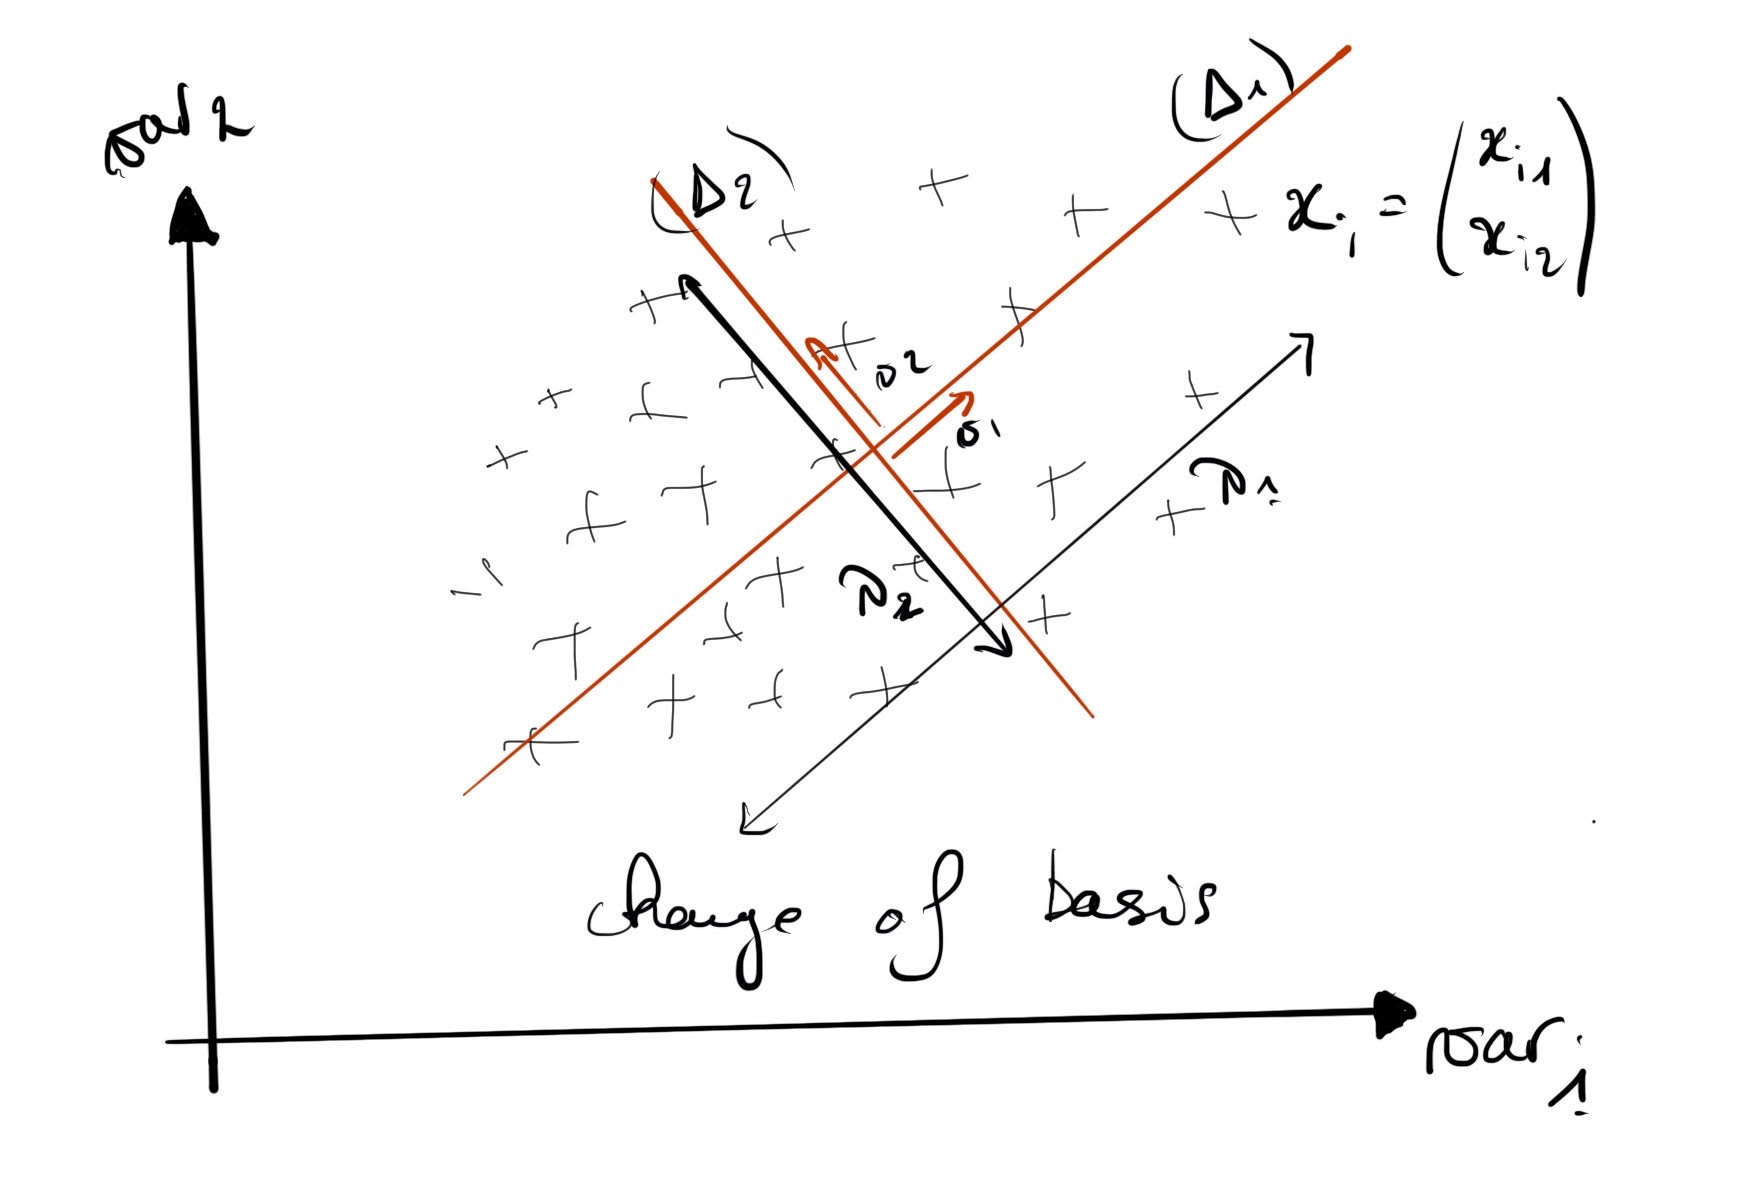
\includegraphics[width=.6\textwidth]{rotation}
\end{frame}

%% ==========================================================================
%% Representation and interpretation
%% ==========================================================================

\section{Representation and interpretation}

\subsection{Quality of the reconstruction}

\begin{frame}
  \frametitle{Contribution of each axis and quality of the representation}
  
  $\Delta_k$ is carrying inertia/variance defined by its orthogonal, thus 
  \begin{equation*}
      I_T = I_{\Delta_1^\bot} + \dots + I_{\Delta_p^\bot} = \lambda_1 + \dots + \lambda_p
  \end{equation*}

  \begin{block}{Relative contribution of axis $k$}<2->
    \vspace{-.5cm}
  \[ 
    \mathrm{contrib}(\Delta_k) = \frac{\lambda_k}{\sum_{k=1}^p\lambda_j} = \frac{\lambda_k}{\trace{\hat\bSigma}} \times 100 
  \]
    $^\rightsquigarrow$ \alert{Percentage of explained inertia/variance explained}
  \end{block}

  \begin{block}{Global quality of the representation on the first $k$ axes}<3->
    \vspace{-.5cm}
  \[ 
    \mathrm{contrib}(\Delta_1,\dots,\Delta_k) = \frac{\lambda_1 + \dots + \lambda_k}{\trace{\hat\bSigma}}  \times 100 
  \]
    A few axes may explain a large proportion of the total variance.\\
    $\rightsquigarrow$ \alert{This paves the way for dimension reduction} 
  \end{block}
  
\end{frame}

\begin{frame}[fragile]
  \frametitle{Scree plot: 'crabs'}

\begin{knitrout}\scriptsize
\definecolor{shadecolor}{rgb}{0.969, 0.969, 0.969}\color{fgcolor}\begin{kframe}
\begin{alltt}
\hlstd{scRNA_pca} \hlkwb{<-} \hlstd{scRNA} \hlopt
  \hlkwd{PCA}\hlstd{(}\hlkwc{graph} \hlstd{=} \hlnum{FALSE}\hlstd{,} \hlkwc{quali.sup} \hlstd{=} \hlkwd{which}\hlstd{(}\hlkwd{colnames}\hlstd{(scRNA)} \hlopt{==} \hlstr{"cell_type"}\hlstd{))}
\hlkwd{fviz_eig}\hlstd{(scRNA_pca)}
\end{alltt}
\end{kframe}
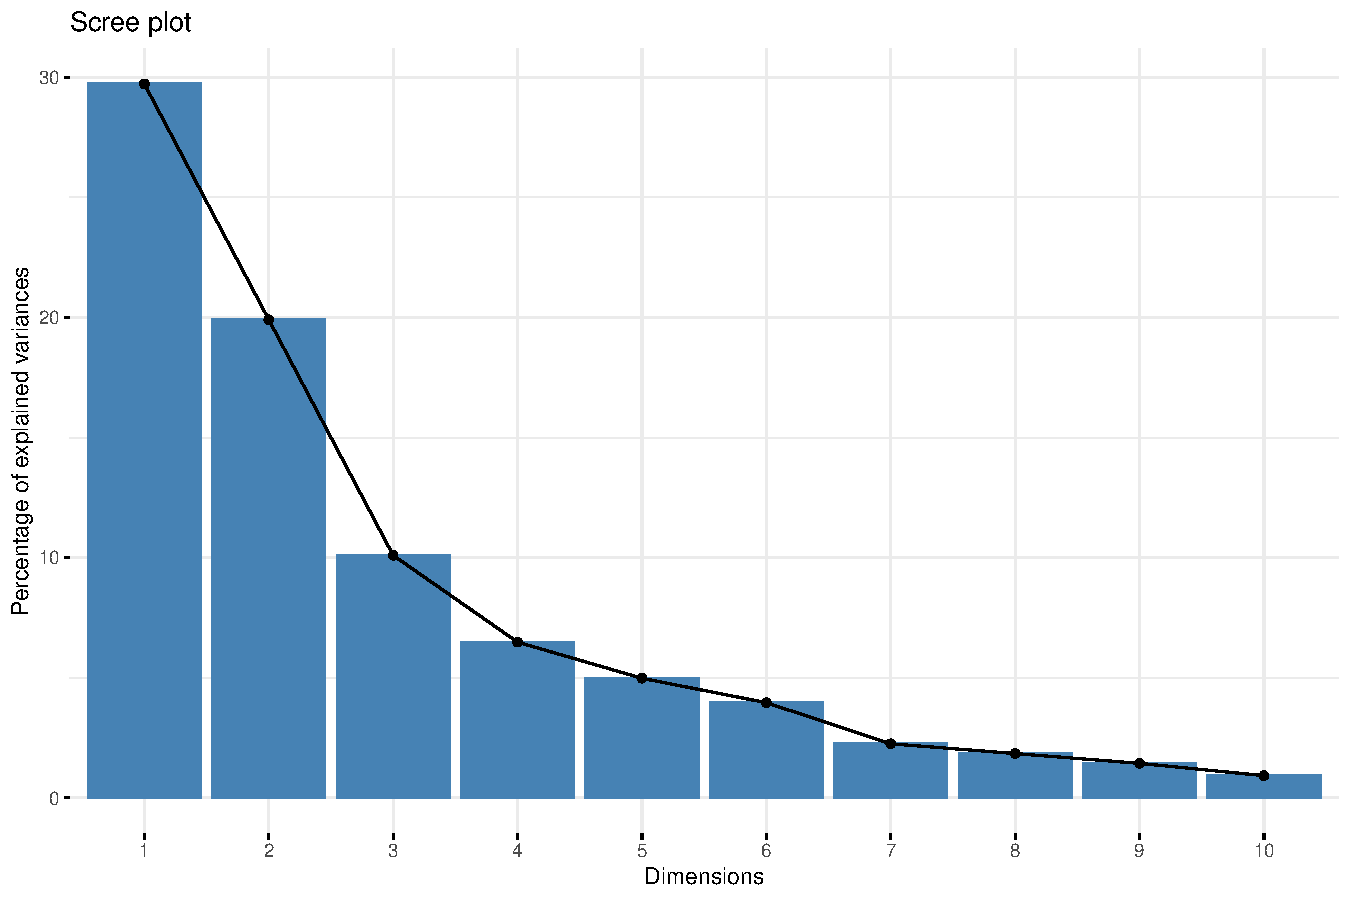
\includegraphics[width=.8\textwidth]{figures/pca_scRNA_screeplot-1} 
\end{knitrout}

\end{frame}

\subsection{Individuals point of view}

\begin{frame}
  \frametitle{Individuals: representation in the new basis}

  \begin{block}{Projection of point $\bx_i$ axis $k$}
    The projection of $\bx_i$ onto axis $\Delta_k$ is $c_{ik} \bv_k$, with 
    \begin{equation*}
      c_{ik} = \bv_k^\top (\bx_i - \bar{\bx}),
    \end{equation*}
     the coordinate of $i$ in the basis $\bv_k$ (along axis $\Delta_k$).
  \end{block}

  \begin{block}{Coordinates of $i$ in the new basis}
    Coordinates of $i$ in the new basis $\{\bv_1, \dots, \bv_p\}$ is thus 
    \begin{equation*}
      \bc_i  = (\bV^\top (\bx_i - \bar{\bx}))^\top = (\bx_i - \bar{\bx})^\top \bV = \bX^c_i \bV, \quad \bc_i \in \Rset^p.
    \end{equation*}

    \begin{itemize}
      \item \alert{$\bV$ are often the called the \textbf{loadings}, or \textbf{weights}}
      \item \alert{$ \bc_i$ are the \textbf{scores} or \textbf{coordinates} in the new space for the individuals}
    \end{itemize}
  \end{block}
\end{frame}


\begin{frame}[fragile]
  \frametitle{Individual visualization: projection in the new basis (1)}

\begin{knitrout}\scriptsize
\definecolor{shadecolor}{rgb}{0.969, 0.969, 0.969}\color{fgcolor}\begin{kframe}
\begin{alltt}
\hlkwd{fviz_pca_ind}\hlstd{(scRNA_pca,} \hlkwc{habillage} \hlstd{=} \hlstr{"cell_type"}\hlstd{)}
\end{alltt}
\end{kframe}
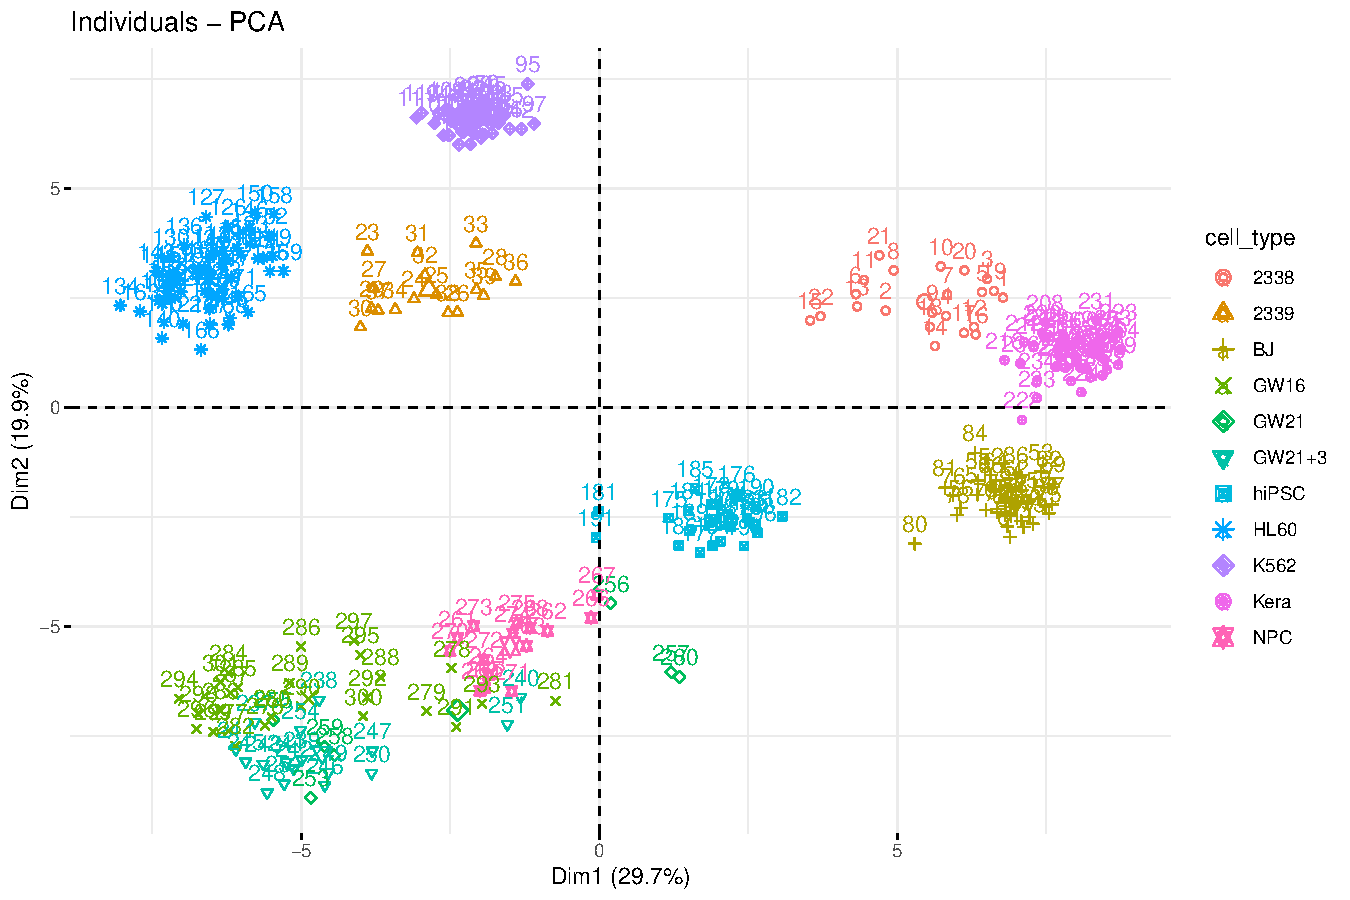
\includegraphics[width=.8\textwidth]{figures/pca_crabs_indmap1-1} 
\end{knitrout}

\end{frame}

\begin{frame}[fragile]
  \frametitle{Individual visualization: projection in the new basis (2)}

\begin{knitrout}\scriptsize
\definecolor{shadecolor}{rgb}{0.969, 0.969, 0.969}\color{fgcolor}\begin{kframe}
\begin{alltt}
\hlkwd{fviz_pca_ind}\hlstd{(scRNA_pca,} \hlkwc{axes} \hlstd{=} \hlkwd{c}\hlstd{(}\hlnum{2}\hlstd{,}\hlnum{3}\hlstd{),} \hlkwc{habillage} \hlstd{=} \hlstr{"cell_type"}\hlstd{)}
\end{alltt}
\end{kframe}
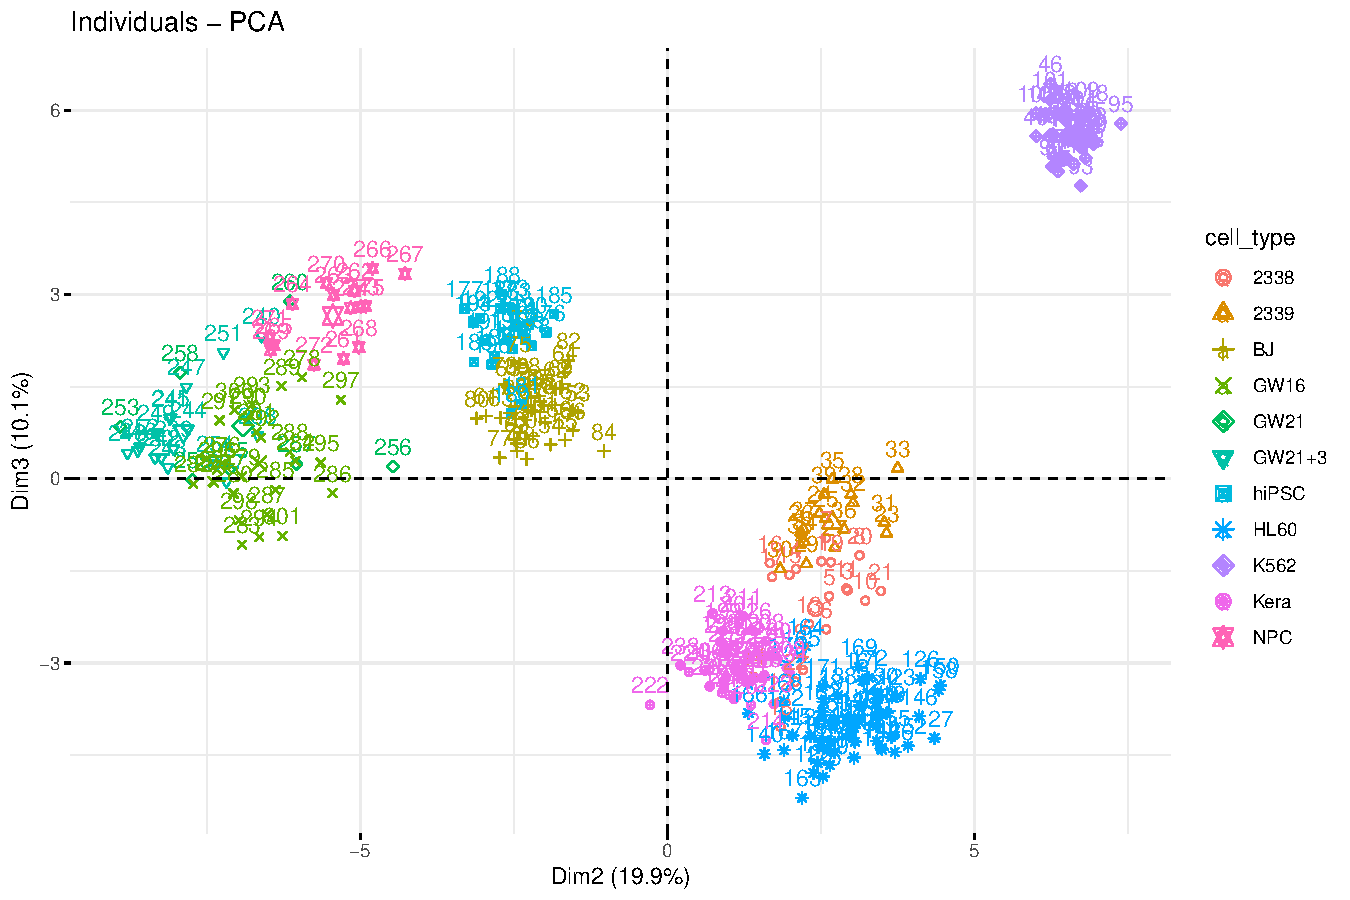
\includegraphics[width=.8\textwidth]{figures/pca_crabs_indmap2-1} 
\end{knitrout}

\end{frame}

\begin{frame}{Warning: about distances after projection}

  \alert{Close projection doesn't mean close individuals!}

  \begin{figure}
    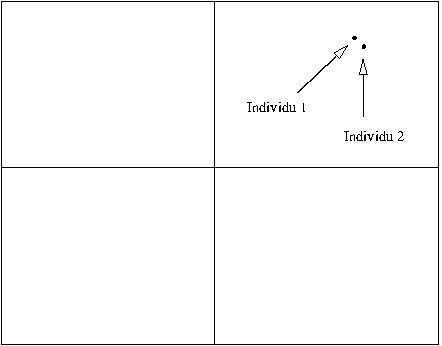
\includegraphics[width = .35\textwidth]{plan_indiv_proche}\\[1ex]
    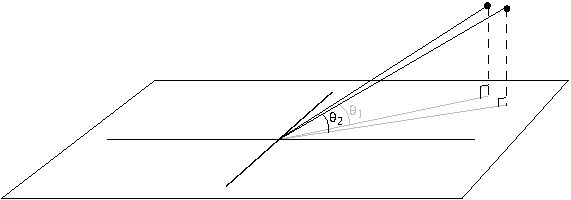
\includegraphics[width = .35\textwidth]{plan_3d_proche}
    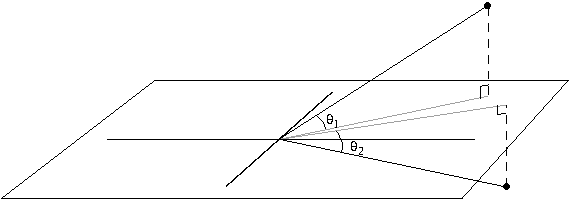
\includegraphics[width = .35\textwidth]{plan_3d_eloigne}
    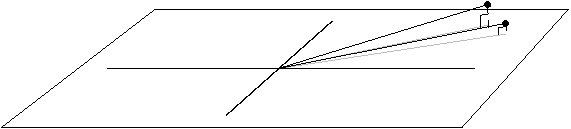
\includegraphics[width = .35\textwidth]{plan_3d_proche2}
    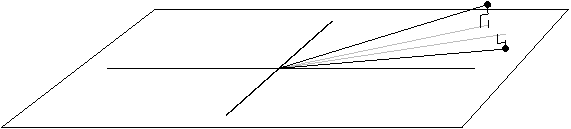
\includegraphics[width = .35\textwidth]{plan_3d_eloigne2}
    \caption{Same projections but different situations {\tiny (source: E. Matzner)}}

  \end{figure}

 $\rightsquigarrow$ Only work when individuals are well represented in the lower space
\end{frame}

\begin{frame}[fragile]
  \frametitle{Individual: quality of the representation}
  
  \begin{block}{Property}
    \begin{itemize}
      \item  An individual $i$ is well represented by $\Delta_k$ if it is close to this axis.
      \item  In other word, vector $\bx_i - \bar{\bx}$ and $\bv_k$ are close to collinear
    \end{itemize}
  \end{block}
 
     We use the cosine of the angle $\theta_{ik}$ between $\bx_i - \bar{\bx}$ and $\bv_k$ to measure the degree of co-linearity:
     \begin{equation*}
       \cos^2(\theta_{ik}) = \frac{\bigg(\bv_k^\top (\bx_i - \bar{\bx})\bigg)^2}{\|\bx_i - \bar{\bx} \|^2 \xout{\|\bv_k \|^2}}
     \end{equation*}

\begin{knitrout}\scriptsize
\definecolor{shadecolor}{rgb}{0.969, 0.969, 0.969}\color{fgcolor}\begin{kframe}
\begin{alltt}
\hlstd{factoextra}\hlopt{::}\hlkwd{get_pca_ind}\hlstd{(scRNA_pca)}\hlopt{$}\hlstd{cos2} \hlopt \hlkwd{head}\hlstd{(}\hlnum{3}\hlstd{)} \hlopt \hlkwd{kable}\hlstd{(}\hlstr{"latex"}\hlstd{)}
\end{alltt}
\end{kframe}
\begin{tabular}{r|r|r|r|r}
\hline
Dim.1 & Dim.2 & Dim.3 & Dim.4 & Dim.5\\
\hline
0.3976361 & 0.0545911 & 0.0156510 & 0.0949606 & 0.0040849\\
\hline
0.1946920 & 0.0412816 & 0.0815729 & 0.2278256 & 0.0000568\\
\hline
0.4160489 & 0.0849204 & 0.0324573 & 0.0912393 & 0.0327544\\
\hline
\end{tabular}

\end{knitrout}
\end{frame}

\begin{frame}[fragile]
  \frametitle{Individual: contribution to an axis}


  \begin{block}{Property}
    \begin{itemize}
      \item Inertia "explained" by $\Delta_k$ is inertia of $\Delta_k^\bot$
      \item $I_{\Delta_k^\bot} = n^{-1}\sum_{i=1}^n \distance^2(\Delta_k^\bot, \bx_i) $
    \end{itemize}
  \end{block}
 
     Contribution of $\bx_i$ to axis $\Delta_k$ is the proportion of variance/inertia carried by individual $i$:
     \begin{equation*}
       \mathrm{contr} (\bx_i) = \frac{n^{-1}\distance^2(\Delta_k^\bot, \bx_i)}{I_{\Delta_k^\bot}} = \frac{\bigg(\bv_k^\top (\bx_i - \bar{\bx})\bigg)^2}{n\lambda_k} 
     \end{equation*}


\begin{knitrout}\scriptsize
\definecolor{shadecolor}{rgb}{0.969, 0.969, 0.969}\color{fgcolor}\begin{kframe}
\begin{alltt}
\hlstd{factoextra}\hlopt{::}\hlkwd{get_pca_ind}\hlstd{(scRNA_pca)}\hlopt{$}\hlstd{contr} \hlopt \hlkwd{head}\hlstd{(}\hlnum{3}\hlstd{)} \hlopt \hlkwd{kable}\hlstd{(}\hlstr{"latex"}\hlstd{)}
\end{alltt}
\end{kframe}
\begin{tabular}{r|r|r|r|r}
\hline
Dim.1 & Dim.2 & Dim.3 & Dim.4 & Dim.5\\
\hline
0.5131474 & 0.1051793 & 0.0594716 & 0.5619077 & 0.0314858\\
\hline
0.2582327 & 0.0817469 & 0.3185806 & 1.3855779 & 0.0004498\\
\hline
0.4731939 & 0.1441978 & 0.1086970 & 0.4758193 & 0.2225046\\
\hline
\end{tabular}

\end{knitrout}
  
\end{frame}

\subsection{Variables point of view}

\begin{frame}
  \frametitle{Cloud of variables in $\Rset^n$}
  
  \begin{center}
    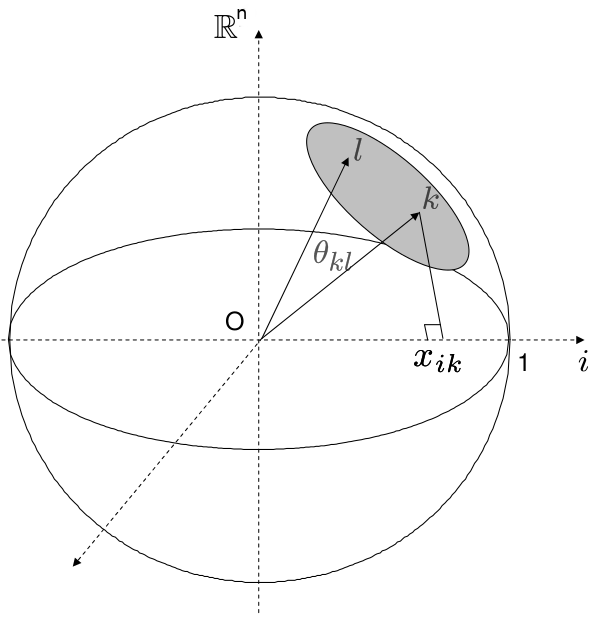
\includegraphics[width=.45\textwidth]{nuage_var}
  \end{center}

  Direct equivalence between geometry and statistics (collinearity $\equiv$ correlation) 
  \begin{equation*}
    \cos(\theta_{kl}) = \frac{\langle \bx^k ,\bx^\ell \rangle}{\|\bx^k\| \|\bx^\ell\|} = \rho(\bx^k,\bx^\ell)
  \end{equation*}

\end{frame}

\begin{frame}
  \frametitle{Principal Components}
  
  \begin{block}{Dual representation}
    A symmetric reasoning can be made in $\Rset^n$ for the variables, like with the individuals in $\Rset^p$.
    
    $\rightsquigarrow$ New axes are linear combinaison of the original variables, which can be seen as \alert{\bf new variables} in the new latent space
  \end{block}

  \begin{block}{Principal component}
    It is the linear combinasion formed by the orginal variables with weights given by the loadings $\bv_k = (v_{k1}, \dots, v_{kj}, \dots, v_{kp})$
    \begin{equation*}
      \mathbf{f}_{k}  = \sum_{j=1}^p v_{kj} (\bx^{j} - \bar{x}_j) = \bX^c \bv_k, \quad \mathbf{f}_k \in \Rset^n
    \end{equation*}
    Sometimes called \alert{"factors"} in  factor analysis, as \alert{latent (hidden) variables}. 
  \end{block}

\end{frame}

\begin{frame}
  \frametitle{Variable representation in the new space}
  
  \begin{block}{Connection with original variables}
    \begin{itemize}
      \item essential for interpretation
      \item answer to the question: how to read the axes of the individual map
      \item use correlation to measure connection to original variable
    \end{itemize}
  \end{block}

  \begin{equation*}
    \var(\mathbf{f}_k) = \bv_k^\top \frac{1}{n}(\bX^c)^\top \bX^c \bv_k =  \bv_k^\top \hat{\bSigma} \bv_k = \lambda_k
  \end{equation*}
  
  \begin{equation*}
    \cov(\mathbf{f}_k, (\bx^j - \bar{x}_j)) = \frac{1}{n}\bv_k \top {\bX^c}^\top \bX^c e_j =  \lambda_k \bv_k^\top e_j = \lambda_k \, v_{kj}   
  \end{equation*}

  \begin{equation*}
    \cor(\mathbf{f}_k, (\bx^j - \bar{x}_j)) =  \sqrt{\frac{\lambda_k}{\var(\bx^j)}} v_{kj}
  \end{equation*}
  
\end{frame}

\begin{frame}[fragile]
  \frametitle{Variable vizualisation: correlation circle (1)}

\begin{knitrout}\scriptsize
\definecolor{shadecolor}{rgb}{0.969, 0.969, 0.969}\color{fgcolor}\begin{kframe}
\begin{alltt}
\hlkwd{fviz_pca_var}\hlstd{(scRNA_pca)}
\end{alltt}
\end{kframe}
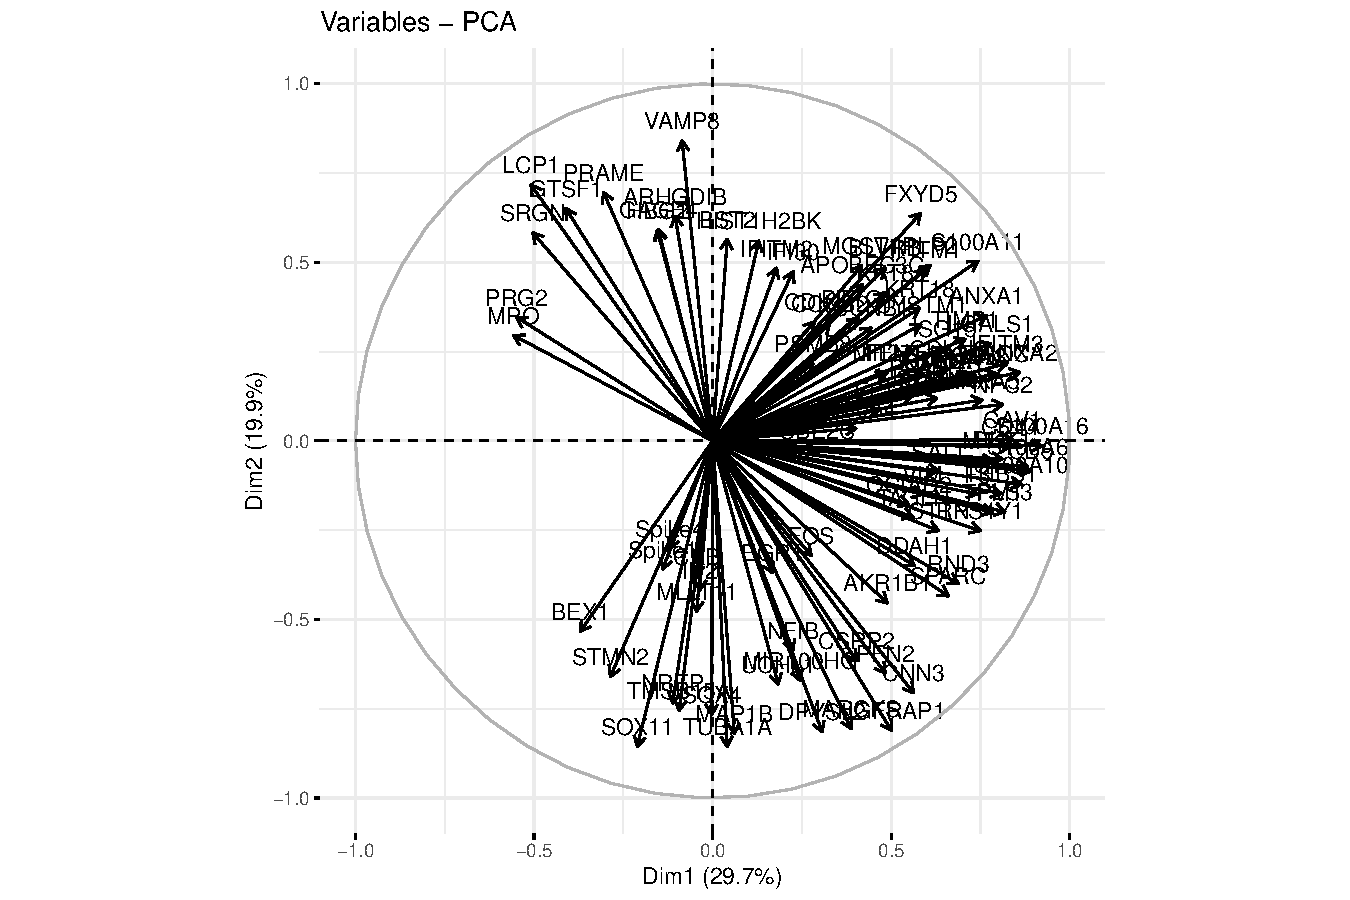
\includegraphics[width=.8\textwidth]{figures/pca_crabs_varmap1-1} 
\end{knitrout}

\end{frame}

\begin{frame}[fragile]
  \frametitle{Variable vizualisation: correlation circle (2)}

\begin{knitrout}\scriptsize
\definecolor{shadecolor}{rgb}{0.969, 0.969, 0.969}\color{fgcolor}\begin{kframe}
\begin{alltt}
\hlkwd{fviz_pca_var}\hlstd{(scRNA_pca,} \hlkwc{axes} \hlstd{=} \hlkwd{c}\hlstd{(}\hlnum{2}\hlstd{,}\hlnum{3}\hlstd{))}
\end{alltt}
\end{kframe}
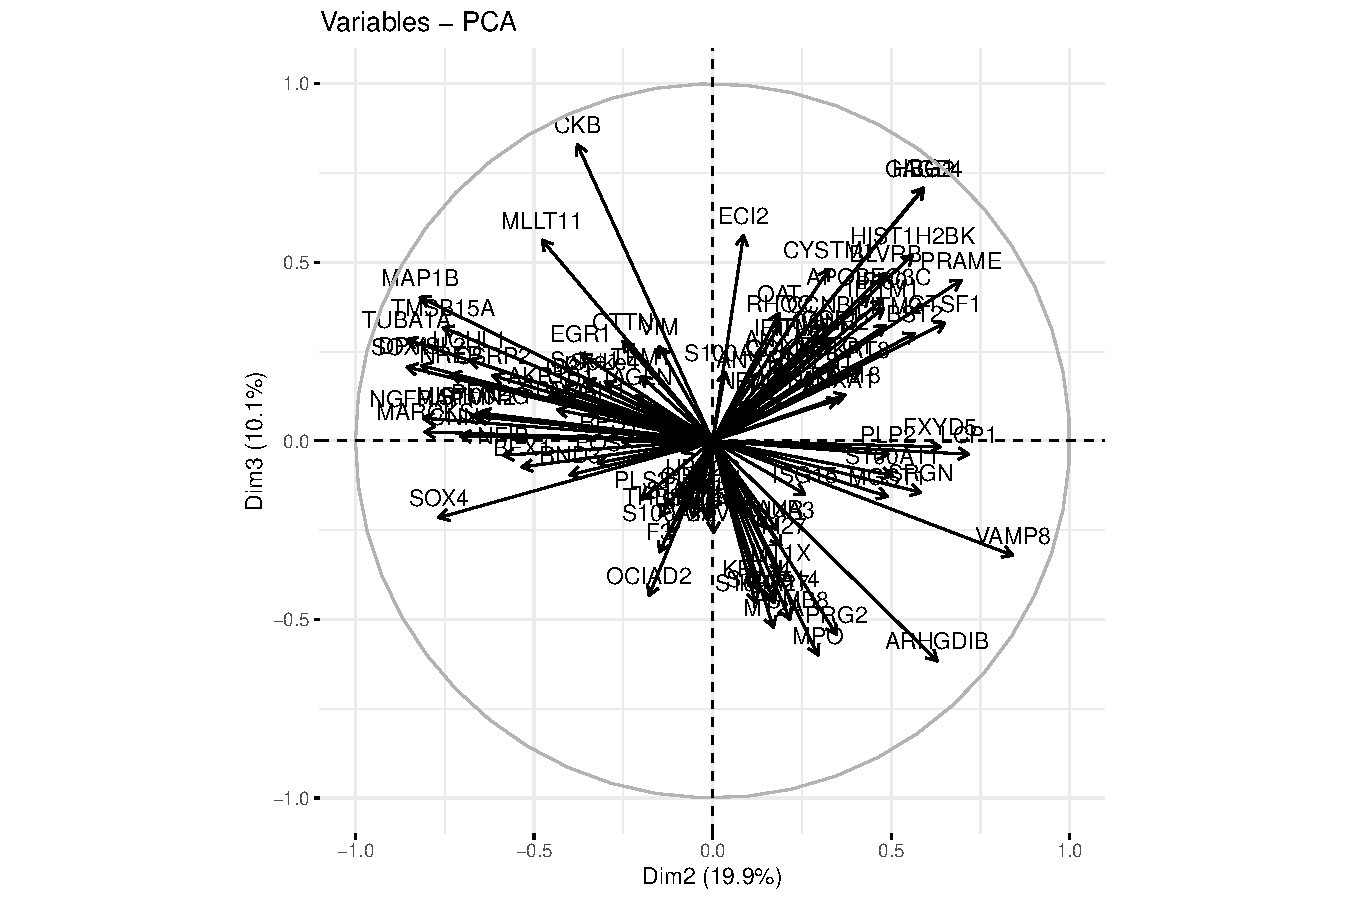
\includegraphics[width=.8\textwidth]{figures/pca_crabs_varmap2-1} 
\end{knitrout}

\end{frame}

\begin{frame}{Warning: about angle after projection}

  \alert{Close projection doesn't mean close variable!}

  \begin{figure}
    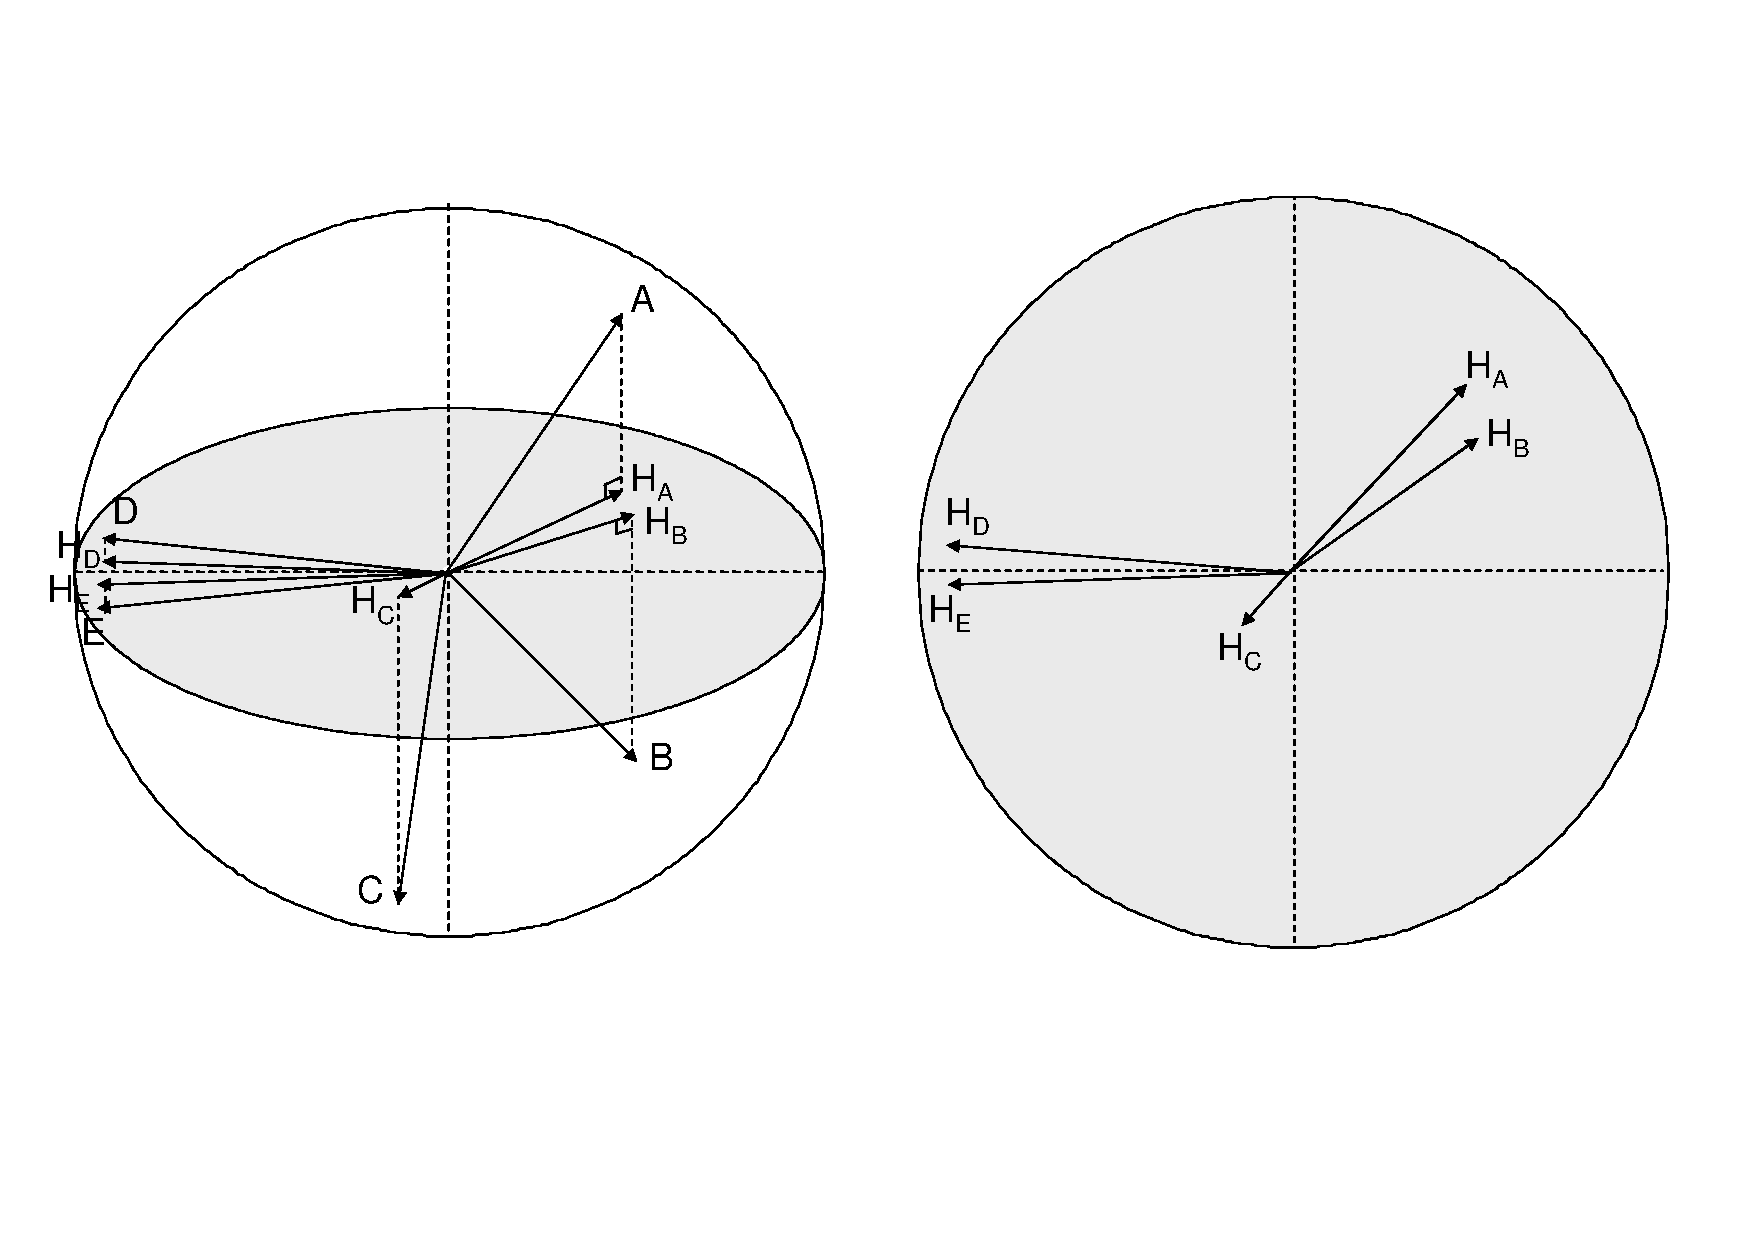
\includegraphics[width = .85\textwidth]{proj_var_acp}
    \caption{Same angle but different situations {\tiny (source: J. Josse)}}

  \end{figure}

 $\rightsquigarrow$ Only work when variables are well represented in the latent space
\end{frame}

\begin{frame}[fragile]
  \frametitle{Variable: quality of the representation}

  Same story as for individuals
  \begin{block}{Property}
    \begin{itemize}
      \item  An variable $j$ is well represented by $\Delta_k$ if its projection is close to $\mathbf{f}_k$.
      \item  High collinearity means high absolute correlation and high cosine.
      \item  use cosine to the square of the angle between the original and new variables.
    \end{itemize}
   $\rightsquigarrow$ The projection of $j$ must be close to the boundady of the correlation circle
  \end{block}
 
\begin{knitrout}\scriptsize
\definecolor{shadecolor}{rgb}{0.969, 0.969, 0.969}\color{fgcolor}\begin{kframe}
\begin{alltt}
\hlstd{factoextra}\hlopt{::}\hlkwd{get_pca_var}\hlstd{(scRNA_pca)}\hlopt{$}\hlstd{cos2} \hlopt \hlkwd{head}\hlstd{(}\hlnum{3}\hlstd{)} \hlopt \hlkwd{kable}\hlstd{(}\hlstr{"latex"}\hlstd{)}
\end{alltt}
\end{kframe}
\begin{tabular}{l|r|r|r|r|r}
\hline
  & Dim.1 & Dim.2 & Dim.3 & Dim.4 & Dim.5\\
\hline
Spike1 & 0.0196220 & 0.1287491 & 0.0292639 & 0.0206783 & 0.6007645\\
\hline
MT2A & 0.4428833 & 0.0290404 & 0.2725646 & 0.0640107 & 0.0344313\\
\hline
HBG2 & 0.0238491 & 0.3478273 & 0.4996552 & 0.0329798 & 0.0343303\\
\hline
\end{tabular}

\end{knitrout}

\end{frame}

\begin{frame}[fragile]
  \frametitle{Variable: contribution to an axis}
  
  Similarly to individuals, we can measure the contribution of the original variables to the construction of the new ones.
  
\begin{knitrout}\scriptsize
\definecolor{shadecolor}{rgb}{0.969, 0.969, 0.969}\color{fgcolor}\begin{kframe}
\begin{alltt}
\hlstd{factoextra}\hlopt{::}\hlkwd{get_pca_var}\hlstd{(scRNA_pca)}\hlopt{$}\hlstd{contr} \hlopt \hlkwd{kable}\hlstd{(}\hlstr{"latex"}\hlstd{)}
\end{alltt}
\end{kframe}
\begin{tabular}{l|r|r|r|r|r}
\hline
  & Dim.1 & Dim.2 & Dim.3 & Dim.4 & Dim.5\\
\hline
Spike1 & 0.0660146 & 0.6466842 & 0.2898943 & 0.3189899 & 12.0718795\\
\hline
MT2A & 1.4899972 & 0.1458647 & 2.7000781 & 0.9874472 & 0.6918700\\
\hline
HBG2 & 0.0802359 & 1.7470759 & 4.9496810 & 0.5087554 & 0.6898405\\
\hline
PRG2 & 1.0139009 & 0.6028304 & 2.9068121 & 1.8379608 & 0.0213405\\
\hline
IFITM1 & 1.2007133 & 1.1528680 & 1.3666546 & 0.7653552 & 1.4680454\\
\hline
ANXA1 & 1.9780804 & 0.6164234 & 0.1320548 & 0.0856922 & 2.6505138\\
\hline
HBG1 & 0.0807819 & 1.7503356 & 4.9690534 & 0.5020974 & 0.6898666\\
\hline
MPO & 1.0457392 & 0.4382956 & 3.5630063 & 1.8958006 & 0.0677635\\
\hline
S100A6 & 2.6183716 & 0.0261683 & 0.3634093 & 0.1959209 & 0.4435930\\
\hline
TUBA1A & 0.0056589 & 3.6825240 & 0.7969656 & 0.0007246 & 0.1601781\\
\hline
ARHGDIB & 0.0371295 & 1.9854261 & 3.7599628 & 0.0232048 & 0.0015973\\
\hline
ANXA2 & 2.4874475 & 0.1862547 & 0.5291199 & 0.0009373 & 0.0726448\\
\hline
LGALS1 & 2.0381581 & 0.3730531 & 0.2802331 & 0.4490980 & 0.6752508\\
\hline
RPS4Y1 & 1.8891255 & 0.3179103 & 0.0000777 & 1.7898114 & 1.1765074\\
\hline
S100A11 & 1.8583855 & 1.2721098 & 0.0928818 & 0.1401025 & 0.0000681\\
\hline
IFITM3 & 2.2872679 & 0.2365565 & 0.6775251 & 0.0247328 & 0.2177227\\
\hline
S100A16 & 2.8571375 & 0.0009453 & 0.4875158 & 0.0048417 & 0.0865240\\
\hline
NGFRAP1 & 0.8430747 & 3.3003985 & 0.0404199 & 0.1031052 & 0.1506221\\
\hline
SRGN & 0.8530570 & 1.7061897 & 0.2069354 & 3.6296214 & 0.7078941\\
\hline
S100A10 & 2.5143552 & 0.0737843 & 0.6556511 & 0.2681132 & 0.0473028\\
\hline
DPYSL2 & 0.3165704 & 3.3341884 & 0.4404124 & 0.2074974 & 0.0181128\\
\hline
CD44 & 2.3325245 & 0.0014708 & 0.4589641 & 0.2843117 & 1.9226148\\
\hline
S100A2 & 1.3268173 & 0.0719245 & 2.0356740 & 0.9910550 & 0.0481329\\
\hline
CKB & 0.0064669 & 0.7213089 & 6.8242077 & 0.0284117 & 0.0022532\\
\hline
SOX11 & 0.1496241 & 3.6756525 & 0.4238253 & 1.0102724 & 0.4155586\\
\hline
MARCKS & 0.5068114 & 3.2614190 & 0.0062172 & 0.3869912 & 0.0747773\\
\hline
CSRP2 & 0.5449854 & 1.9018112 & 0.3306449 & 0.0505356 & 0.9753511\\
\hline
CAV1 & 2.3718320 & 0.0000482 & 0.6526089 & 0.3015961 & 1.4633750\\
\hline
Spike4 & 0.0485343 & 0.4557218 & 0.2743835 & 0.5675750 & 12.3050005\\
\hline
VAMP8 & 0.0245161 & 3.5468203 & 1.0187765 & 0.3324101 & 0.8591847\\
\hline
KRT18 & 1.1274319 & 0.6921348 & 0.1648909 & 3.4792296 & 2.2206004\\
\hline
UCHL1 & 0.1138161 & 2.3291668 & 0.5116918 & 1.5124236 & 0.1125936\\
\hline
F3 & 1.8480657 & 0.1112939 & 0.9579382 & 1.0115384 & 0.2629204\\
\hline
TMSB15A & 0.0294735 & 2.8625550 & 0.9985516 & 0.0000006 & 2.0518146\\
\hline
PRAME & 0.3138535 & 2.4314919 & 1.9995252 & 0.1465705 & 0.4900495\\
\hline
CD9 & 2.6701405 & 0.0356733 & 0.2285499 & 0.0067139 & 0.3865116\\
\hline
UBE2C & 0.2880321 & 0.0038164 & 0.1683445 & 1.8965056 & 7.1987046\\
\hline
MAP1B & 0.0124287 & 3.3694732 & 1.6035984 & 0.0187950 & 0.4353387\\
\hline
IFITM2 & 0.1082458 & 1.1767822 & 1.0339745 & 2.2490729 & 0.2745995\\
\hline
RND3 & 1.5911685 & 0.8018906 & 0.0897981 & 0.1081230 & 0.0368911\\
\hline
SOX4 & 0.0000239 & 2.9519608 & 0.4586023 & 1.3364266 & 0.7945965\\
\hline
VIM & 1.1618316 & 0.1128327 & 0.6880704 & 1.0887802 & 1.0696289\\
\hline
NREP & 0.0419906 & 2.7051550 & 0.3422922 & 0.5698644 & 0.1923092\\
\hline
OCIAD2 & 1.0146613 & 0.1591167 & 1.8570072 & 0.0004870 & 0.5758463\\
\hline
TIMP1 & 1.6815645 & 0.4065051 & 0.6950542 & 1.1044475 & 0.3391455\\
\hline
DKK1 & 2.2129085 & 0.0129478 & 0.3214593 & 1.2192780 & 2.1334138\\
\hline
SPARC & 1.4650720 & 0.9476479 & 0.0754968 & 1.6579063 & 0.0016321\\
\hline
OAT & 1.7930737 & 0.1752172 & 1.2678212 & 0.3205073 & 0.0314091\\
\hline
GAGE4 & 0.0775682 & 1.7547958 & 4.9446809 & 0.5354602 & 0.6895598\\
\hline
KRT14 & 1.0465709 & 0.0769896 & 1.6996161 & 1.2457735 & 0.0070788\\
\hline
MLLT11 & 0.0068329 & 1.1447955 & 3.1315197 & 0.3247333 & 1.0442252\\
\hline
RHOC & 2.1209976 & 0.1795876 & 1.0779874 & 0.0260352 & 0.3233849\\
\hline
PFN2 & 0.7855787 & 2.1227904 & 0.0606607 & 0.0193582 & 0.1106114\\
\hline
BLVRB & 0.7820414 & 1.1788232 & 2.1813800 & 0.5309208 & 0.0298379\\
\hline
THBS1 & 2.1963612 & 0.1088476 & 0.4441442 & 0.4521117 & 2.0193509\\
\hline
TPM1 & 2.0650712 & 0.2013210 & 0.3254021 & 0.2905704 & 0.4605547\\
\hline
ECI2 & 0.7348444 & 0.0374124 & 3.2733821 & 0.9715209 & 0.0139202\\
\hline
BEX1 & 0.4615138 & 1.4297366 & 0.0532678 & 0.7515569 & 0.4436644\\
\hline
MT1E & 2.0736718 & 0.0157115 & 0.4574135 & 0.9718571 & 1.8861367\\
\hline
ANXA3 & 1.7321927 & 0.1651806 & 0.6161690 & 2.3790211 & 0.8014569\\
\hline
MGST1 & 0.5847567 & 1.2054606 & 0.2402264 & 2.0355537 & 0.8499836\\
\hline
CDK1 & 0.2730402 & 0.5579648 & 0.8125146 & 1.5475300 & 1.6198156\\
\hline
GTSF1 & 0.5679440 & 2.1245781 & 1.0771742 & 0.0381996 & 0.1350331\\
\hline
KRT8 & 0.7854089 & 0.8658511 & 0.3901447 & 4.1780960 & 2.3557138\\
\hline
FXYD5 & 1.1403944 & 2.0383516 & 0.0027299 & 0.1493969 & 0.0385141\\
\hline
HIST1H2BK & 0.0561556 & 1.5750489 & 2.6794844 & 1.3596497 & 0.0712440\\
\hline
NFIB & 0.1698572 & 1.7278625 & 0.0162175 & 5.8601148 & 0.5744210\\
\hline
S100A14 & 1.4882099 & 0.1422208 & 1.9301194 & 3.5873767 & 0.2785584\\
\hline
SAT1 & 1.3471302 & 0.0359190 & 0.0105328 & 1.2550333 & 0.0109197\\
\hline
MIR100HG & 0.2030464 & 2.2632608 & 0.0502156 & 0.1723914 & 3.4004722\\
\hline
EGR1 & 0.0944540 & 0.6853382 & 0.5887023 & 0.1705209 & 1.8907086\\
\hline
LCP1 & 0.8703861 & 2.5806991 & 0.0137669 & 0.2957696 & 0.0113046\\
\hline
MT1X & 1.1666604 & 0.1803055 & 1.3394001 & 0.5712225 & 1.0598466\\
\hline
IFI30 & 0.1711040 & 1.1281731 & 1.5347460 & 0.0004402 & 0.0379384\\
\hline
ISG15 & 1.4159095 & 0.3350617 & 0.2201326 & 0.9841909 & 0.3638394\\
\hline
CNN3 & 1.0654938 & 2.4998255 & 0.0017363 & 0.1704038 & 0.2245059\\
\hline
AKR1B1 & 0.8052652 & 1.0344457 & 0.1578391 & 1.4414907 & 0.7206567\\
\hline
CCNB1 & 0.6614739 & 0.5018523 & 1.0583615 & 0.3603646 & 2.6631919\\
\hline
PLS3 & 2.2536496 & 0.1989624 & 0.2642613 & 0.0128638 & 0.0665153\\
\hline
BST2 & 0.0056410 & 1.6038091 & 0.8957728 & 1.6424934 & 1.2472574\\
\hline
CCNB2 & 0.3612659 & 0.5408104 & 0.7685505 & 0.7015723 & 3.5508613\\
\hline
ID2 & 0.0045208 & 0.8778793 & 0.2288080 & 1.9125680 & 1.3507328\\
\hline
DDAH1 & 1.0737891 & 0.6119714 & 0.0772703 & 1.9021399 & 0.0131082\\
\hline
PLP2 & 1.2484377 & 1.2126025 & 0.0141704 & 0.0048470 & 0.8981259\\
\hline
CYSTM1 & 1.1455936 & 0.5341380 & 2.2795610 & 0.0175520 & 0.0058506\\
\hline
ANXA5 & 1.9132182 & 0.0656963 & 0.2954422 & 0.4710167 & 0.0060327\\
\hline
STMN2 & 0.2755938 & 2.1882490 & 0.0467595 & 0.9708897 & 1.5468258\\
\hline
FOS & 0.2564779 & 0.5158117 & 0.0378311 & 0.3499810 & 0.5643320\\
\hline
PTTG1 & 0.5594889 & 0.5941173 & 0.4428833 & 1.9308065 & 3.1191569\\
\hline
KRT17 & 1.3095312 & 0.1499982 & 2.0379528 & 3.2343578 & 0.0177024\\
\hline
IFI27 & 0.7999267 & 0.1831655 & 0.8565341 & 3.7475589 & 0.3091145\\
\hline
PSMB8 & 0.2664412 & 0.2349735 & 2.4738094 & 0.1660994 & 0.2878367\\
\hline
CDKN3 & 1.4599366 & 0.2058761 & 0.4170695 & 0.0894840 & 1.7459206\\
\hline
APOBEC3C & 0.5916072 & 0.9617156 & 1.6247054 & 0.3916778 & 0.0874387\\
\hline
TAGLN & 1.0600888 & 0.2306151 & 0.1557814 & 4.2854527 & 0.3453209\\
\hline
CTTN & 1.3470162 & 0.3174451 & 0.7702415 & 2.7322888 & 0.0950894\\
\hline
S100A4 & 0.5419604 & 0.0062426 & 0.3672996 & 5.2605888 & 0.5704759\\
\hline
NPC2 & 2.2195321 & 0.0524421 & 0.1248858 & 0.0188685 & 0.4932869\\
\hline
MIEN1 & 0.8065209 & 0.1851556 & 0.1423601 & 1.2968603 & 0.1496903\\
\hline
PLAUR & 1.2027298 & 0.1123865 & 0.5920691 & 0.7637293 & 0.6094841\\
\hline
\end{tabular}

\end{knitrout}


\end{frame}

%% ==========================================================================
%% Complements
%% ==========================================================================

\section{Additional tools and Complements}

\begin{frame}[fragile]
  \frametitle{Unifying view of variables and individuals}

  \begin{block}{Principal components}
   The full matrix of principal component connects  individual coordinates to latent factors:
    \begin{equation*}
      \mathrm{PC} = \bX^c \bV = \begin{pmatrix}
      \mathbf{f}_{1} & \mathbf{f}_{2} & \dots & \mathbf{f}_{p}
      \end{pmatrix}
      = \begin{pmatrix} 
      \bc_{1}^\top \\ \bc_{2}^\top \\\dots \\ \bc_{n}^\top 
      \end{pmatrix}
    \end{equation*}
  \end{block}

  \vfill
  
  \begin{itemize}
    \item new variables (latent factor) are seen column-wise
    \item new coordinates are seen row-wise
  \end{itemize}

  $\rightsquigarrow$ Everything can be interpreted on a single plot, called the biplot

\end{frame}

\begin{frame}[fragile]
  \frametitle{Biplot (1)}
\begin{knitrout}\scriptsize
\definecolor{shadecolor}{rgb}{0.969, 0.969, 0.969}\color{fgcolor}\begin{kframe}
\begin{alltt}
  \hlstd{factoextra}\hlopt{::}\hlkwd{fviz_pca_biplot}\hlstd{(scRNA_pca,}
    \hlkwc{axes} \hlstd{=} \hlkwd{c}\hlstd{(}\hlnum{1}\hlstd{,}\hlnum{2}\hlstd{),} \hlkwc{habillage} \hlstd{=} \hlstr{"cell_type"}\hlstd{,}
    \hlkwc{select.var} \hlstd{=} \hlkwd{list}\hlstd{(}\hlkwc{contrib} \hlstd{=} \hlnum{30}\hlstd{)}
  \hlstd{)}
\end{alltt}
\end{kframe}
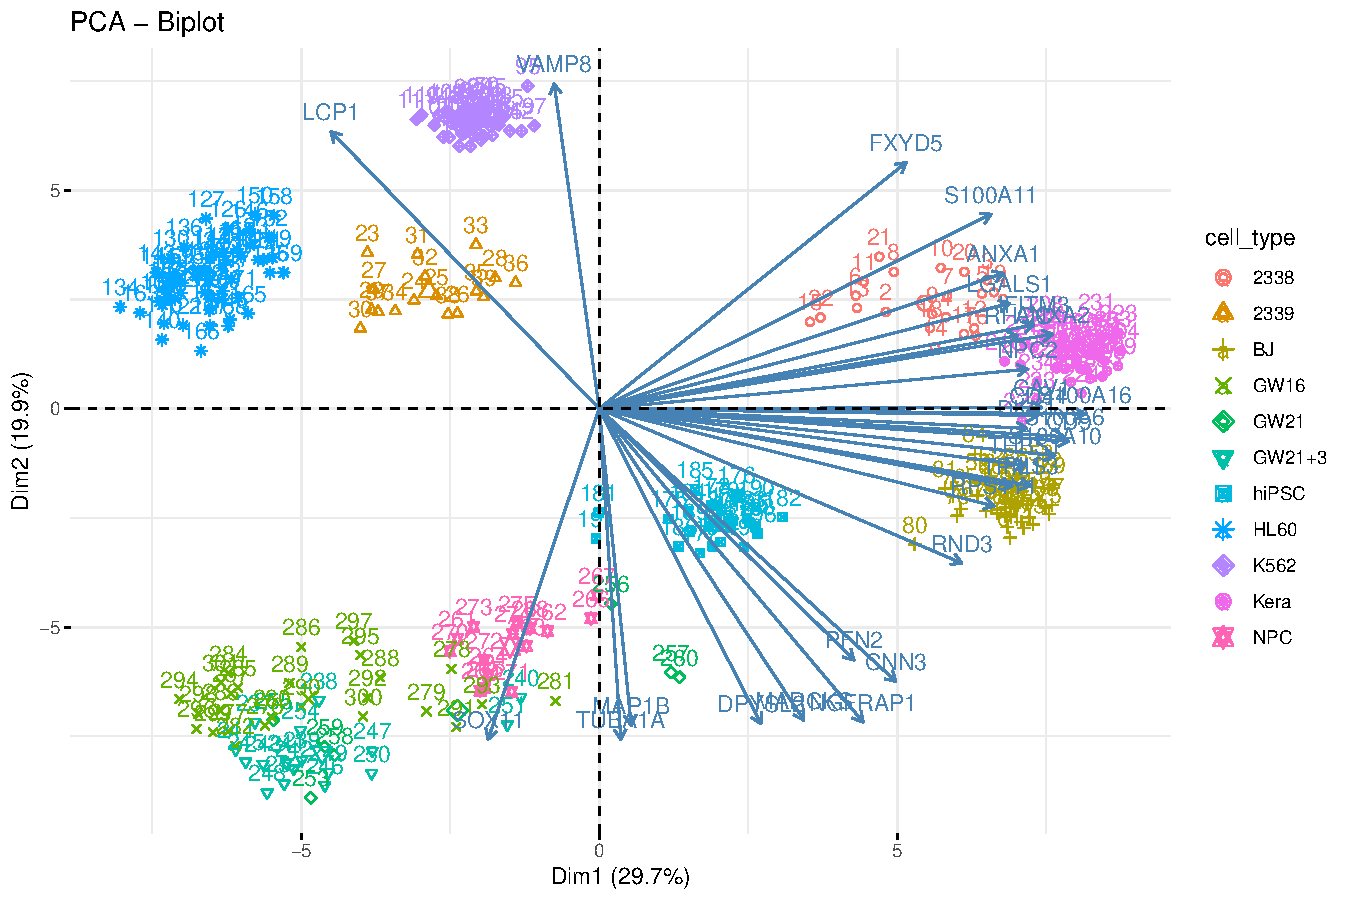
\includegraphics[width=.8\textwidth]{figures/biplot1_scRNA_untransformed-1} 
\end{knitrout}
\end{frame}

\begin{frame}[fragile]
  \frametitle{Biplot (2)}
\begin{knitrout}\scriptsize
\definecolor{shadecolor}{rgb}{0.969, 0.969, 0.969}\color{fgcolor}\begin{kframe}
\begin{alltt}
  \hlstd{factoextra}\hlopt{::}\hlkwd{fviz_pca_biplot}\hlstd{(scRNA_pca,}
    \hlkwc{axes} \hlstd{=} \hlkwd{c}\hlstd{(}\hlnum{2}\hlstd{,}\hlnum{3}\hlstd{),} \hlkwc{habillage} \hlstd{=} \hlstr{"cell_type"}\hlstd{,}
    \hlkwc{select.var} \hlstd{=} \hlkwd{list}\hlstd{(}\hlkwc{cos2} \hlstd{=} \hlnum{.75}\hlstd{)}
  \hlstd{)}
\end{alltt}
\end{kframe}
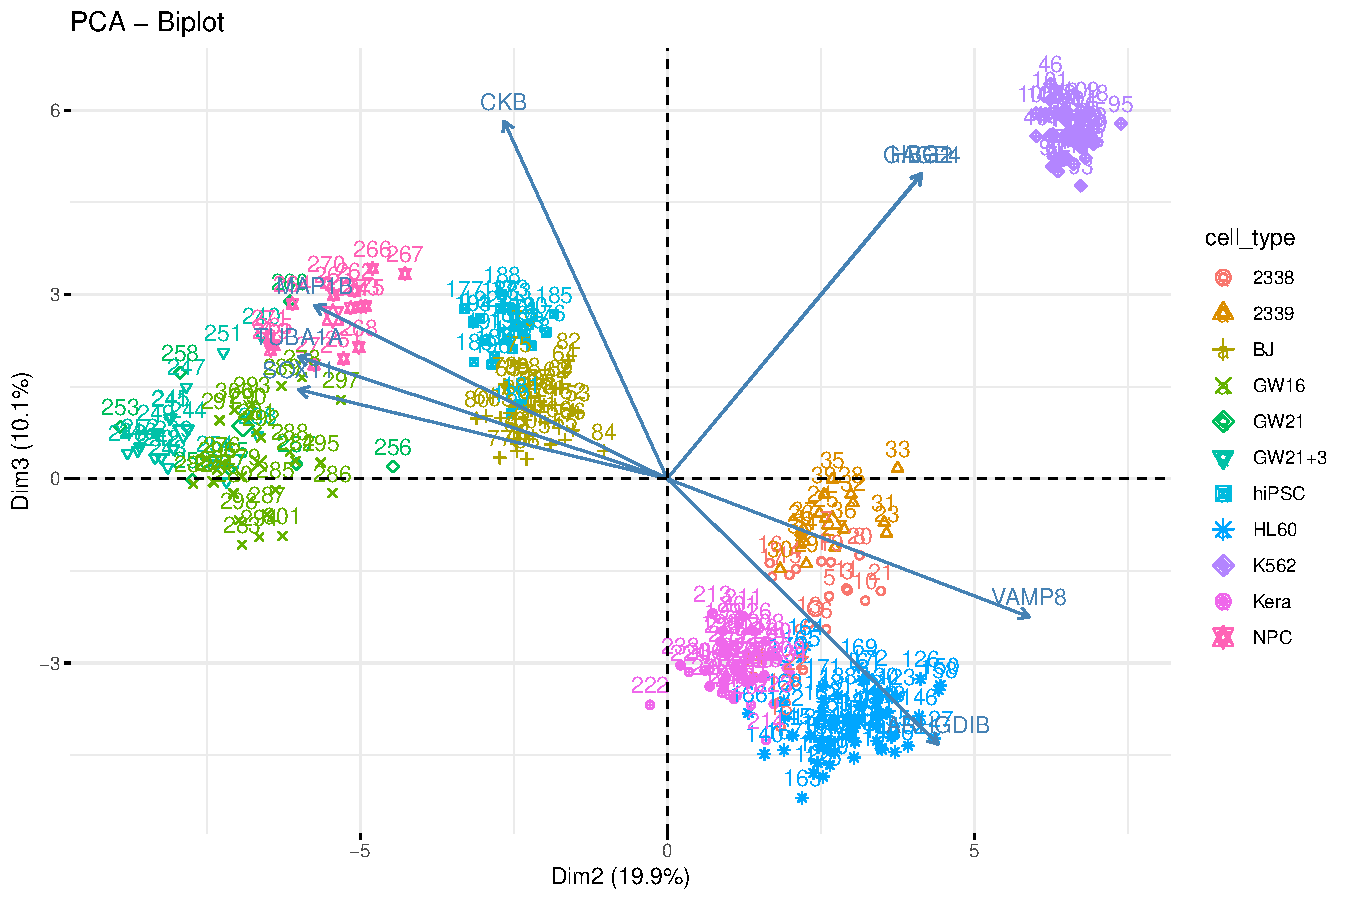
\includegraphics[width=.8\textwidth]{figures/biplot2_scRNA_untransformed-1} 
\end{knitrout}
\end{frame}

\begin{frame}
  \frametitle{Reconstruction formula}

    Recall that $\mathbf{F} = (\mathbf{f}_1, \dots, \mathbf{f}_p) $ is the matrix of Principal components. Then,  
    \begin{itemize}
      \item  $\mathbf{f}_k = \bX^c \bv_k$ for projection on axis $k$
      \item $\mathbf{F} = \bX^c \bV$ for all axis.
    \end{itemize}
    Using orthogonality of $\bV$, we get back the original data as follows, without loss ($\bV^T$ performs the inverse rotation of $\bV$):
    \begin{equation*}
      \bX^c = \mathbf{F}\bV^\top 
    \end{equation*}

    \vfill
    \pause

    We obtain an approximation $\tilde\bX^c$ (compression) of the data $\bX^c$ by considering a subset $\mathcal{S}$ of PC, typically $\mathcal{S} = {1, \dots, q}$ with $q \ll p$.
    \begin{equation*}
      \tilde\bX^c = \mathbf{F}_{\mathcal{S}}\bV_{\mathcal{S}}^\top = \bX^c \bV_{\mathcal{S}} \bV_{\mathcal{S}}^\top
    \end{equation*}
    $\rightsquigarrow$ This is a rank-$q$ approximation of $\bX$ (information captured by the first $q$ axes).

\end{frame}

\begin{frame}
  \frametitle{Choosing the number of components}

  \begin{columns}
  \begin{column}{0.68\textwidth}
    \begin{block}{Various solutions, open question}
    Scree plot, test on eigenvalues, confidence interval, cross-validation, generalized cross-validation, etc.
    \end{block}
  \end{column}~~
  \begin{column}{0.3\textwidth}
    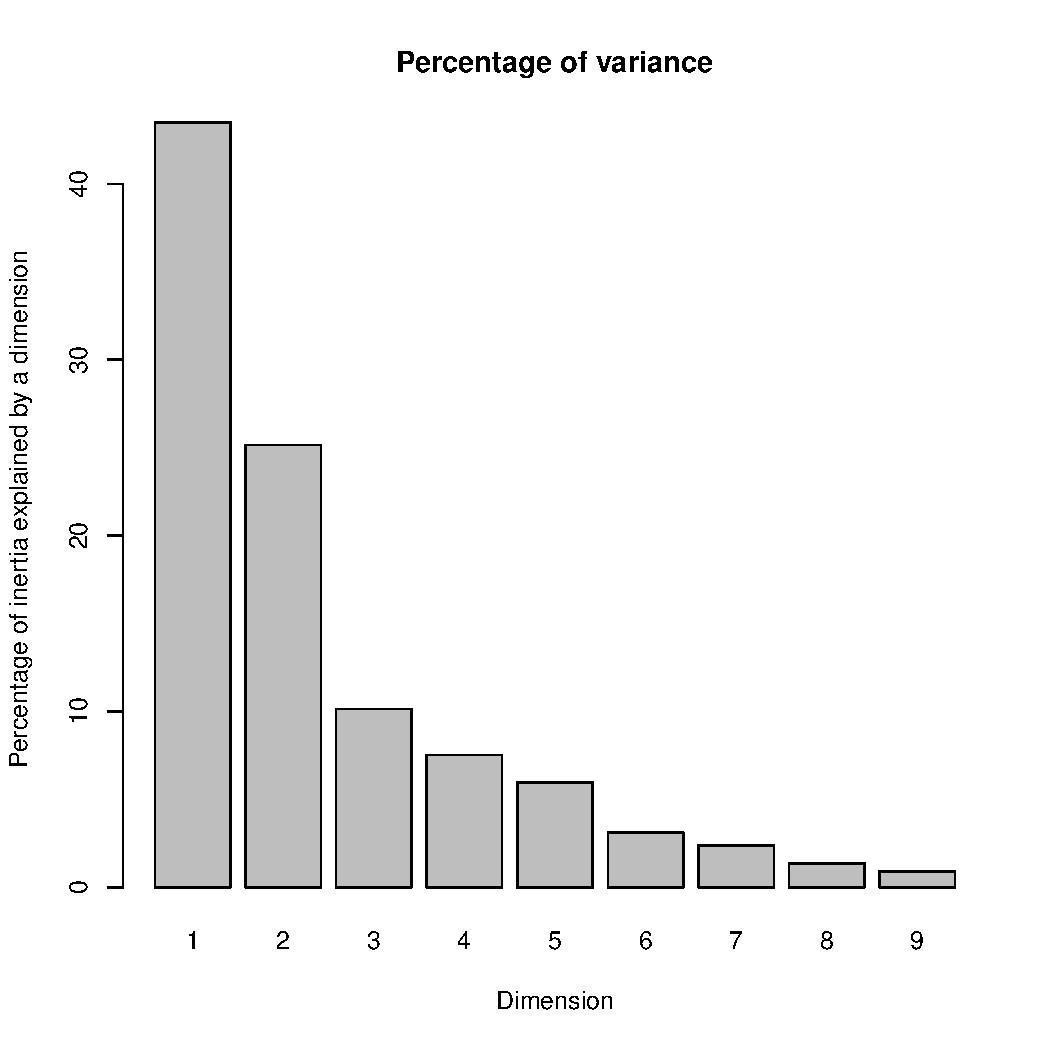
\includegraphics[width=\textwidth]{wine_pca_eig}
  \end{column}
  \end{columns}
  
  \begin{columns}
  \begin{column}{.5\textwidth}
  \begin{block}{Objectives}
    \begin{itemize}
      \item Interpretation
      \item Separate structure and noise
      \item Data compression    
    \end{itemize}
  \end{block}
\end{column}
\begin{column}{0.5\textwidth}
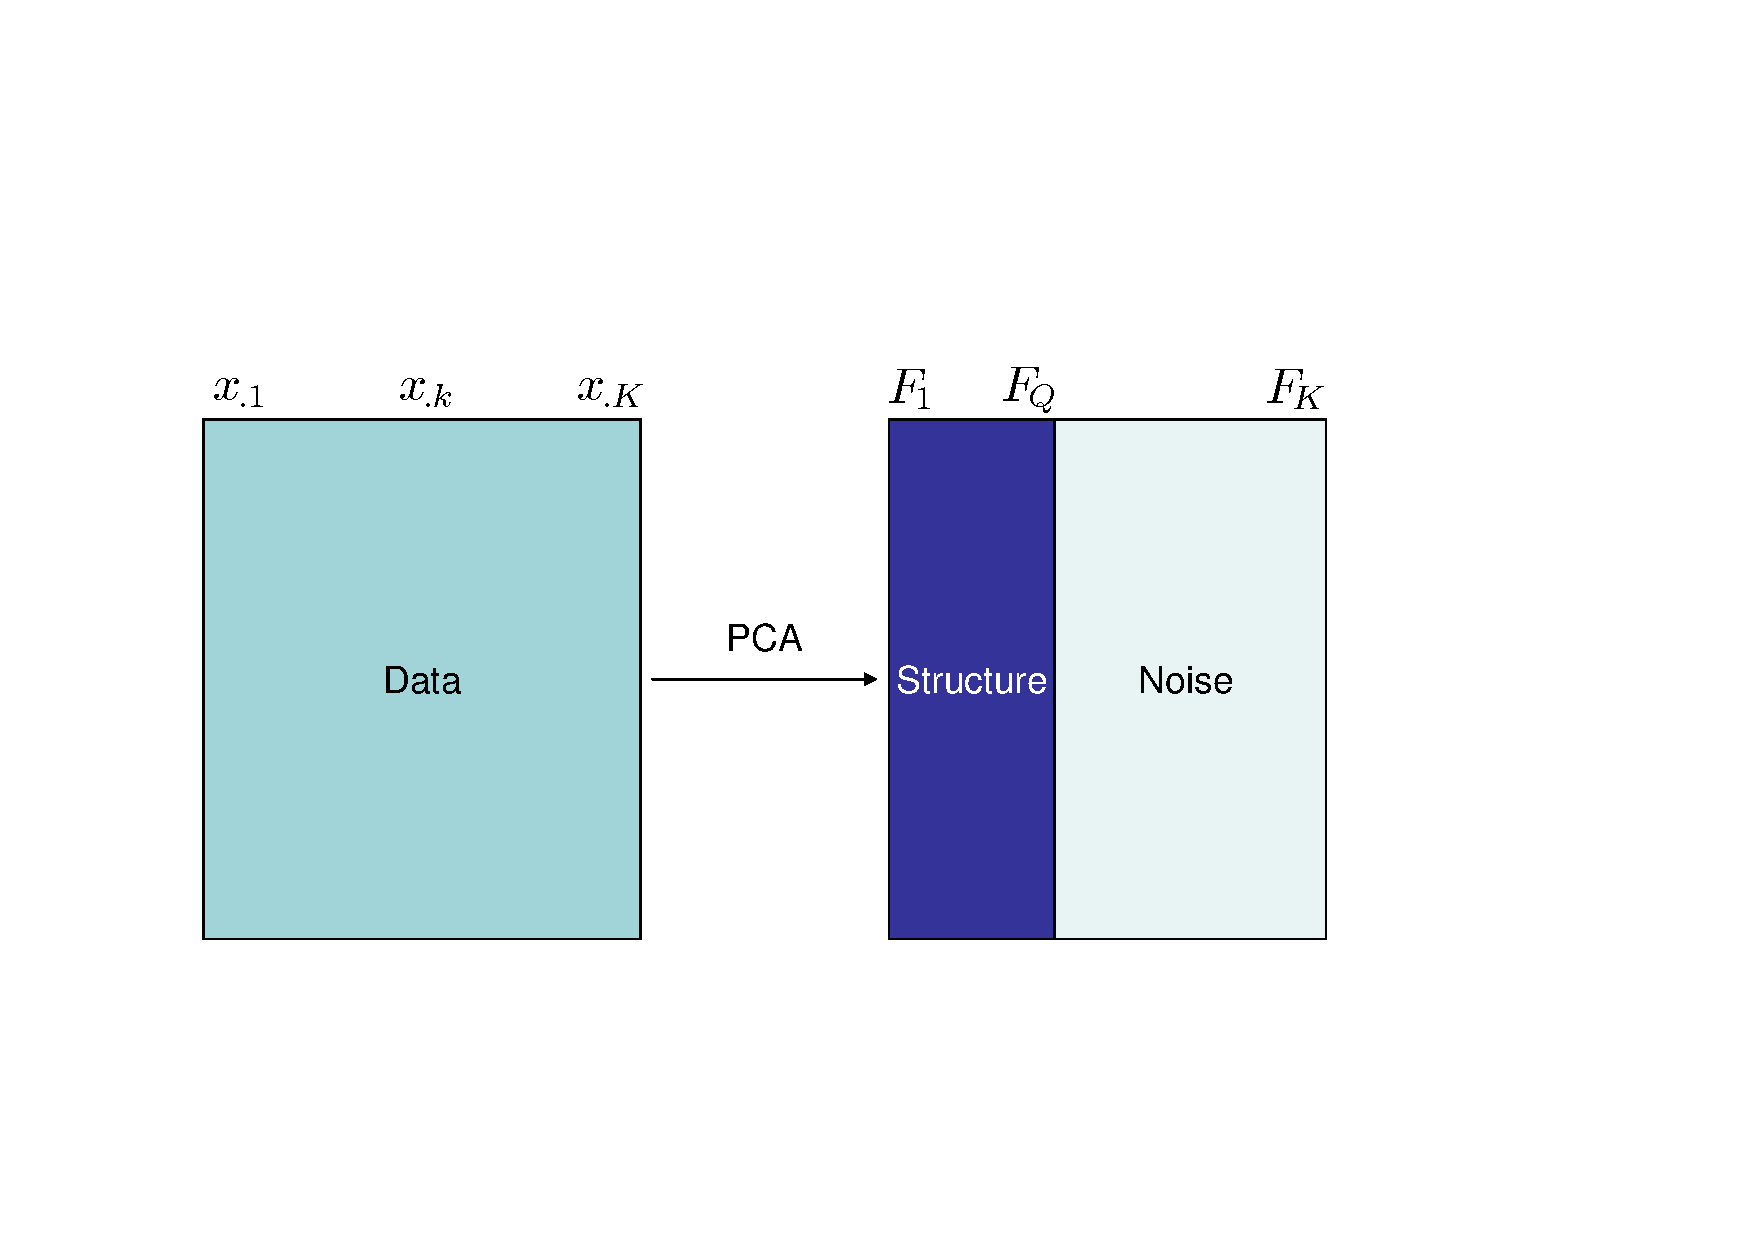
\includegraphics[width=\textwidth]{dim_reduc.pdf}
  \end{column}
  \end{columns}
\end{frame}

\begin{frame}[fragile]
  \frametitle{Example: Generalized Cross Validation}

\begin{knitrout}\scriptsize
\definecolor{shadecolor}{rgb}{0.969, 0.969, 0.969}\color{fgcolor}\begin{kframe}
\begin{alltt}
\hlstd{GCV} \hlkwb{<-} \hlstd{dplyr}\hlopt{::}\hlkwd{select}\hlstd{(scRNA,} \hlopt{-}\hlstd{cell_type)} \hlopt \hlkwd{as.matrix}\hlstd{()} \hlopt
  \hlstd{FactoMineR}\hlopt{::}\hlkwd{estim_ncp}\hlstd{(}\hlkwc{ncp.min} \hlstd{=} \hlnum{1}\hlstd{,} \hlkwc{ncp.max} \hlstd{=} \hlnum{30}\hlstd{)}
\hlkwd{qplot}\hlstd{(}\hlnum{1}\hlopt{:}\hlkwd{length}\hlstd{(GCV}\hlopt{$}\hlstd{criterion), GCV}\hlopt{$}\hlstd{criterion,} \hlkwc{geom} \hlstd{=} \hlstr{"line"}\hlstd{,} \hlkwc{xlab} \hlstd{=} \hlstr{"number of axis"}\hlstd{,} \hlkwc{ylab} \hlstd{=} \hlstr{"GCV"}\hlstd{)}
\end{alltt}
\end{kframe}
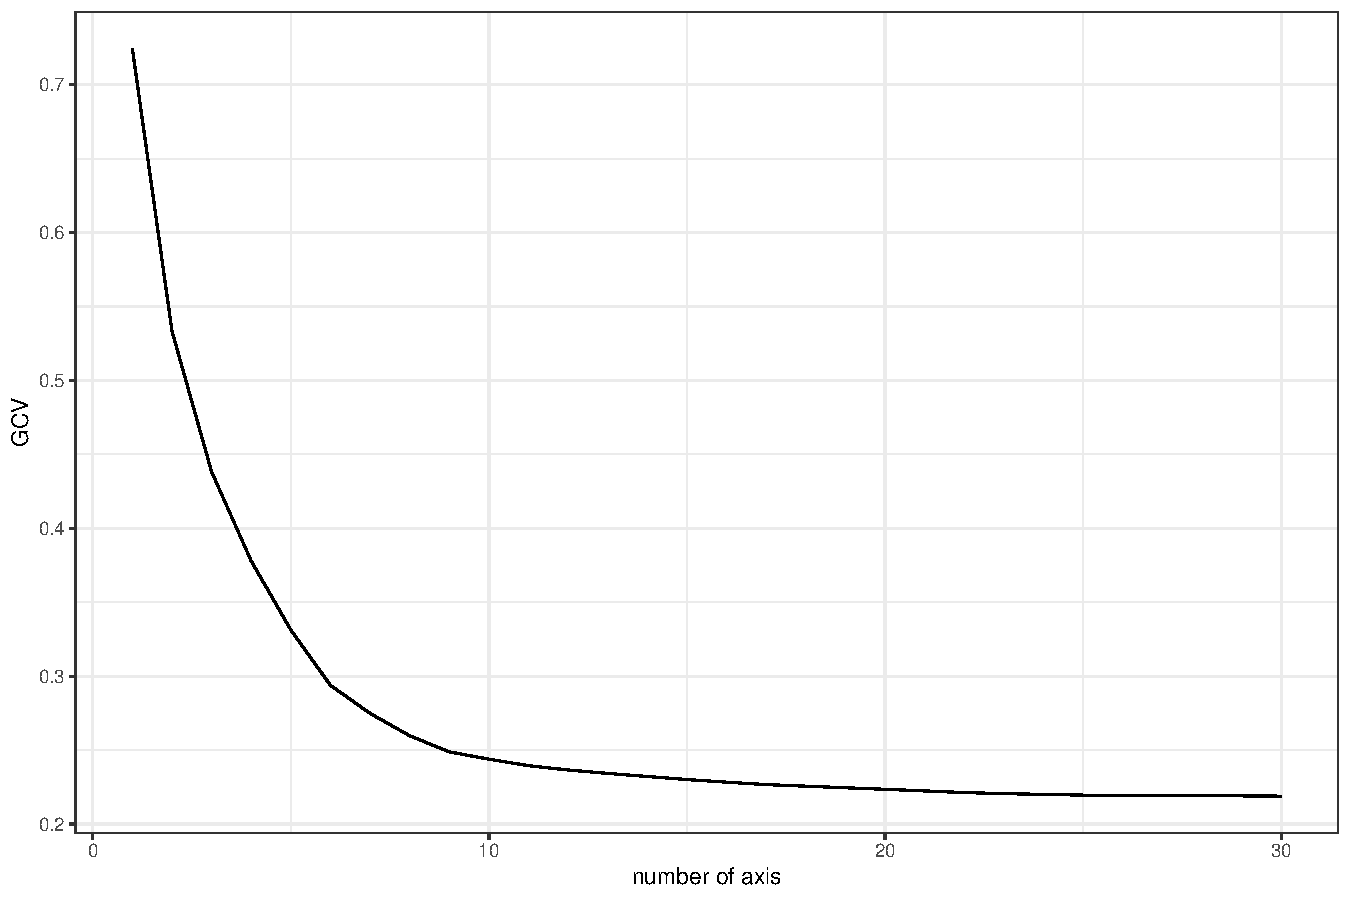
\includegraphics[width=.8\textwidth]{figures/crabs_gcv-1} 
\end{knitrout}
\end{frame}



%% ====================================================================
\part{Non-linear Methods}
%% ====================================================================
\begin{frame}[fragile]
  \partpage

\paragraph{Packages required for reproducing the slides}
\begin{knitrout}\scriptsize
\definecolor{shadecolor}{rgb}{0.969, 0.969, 0.969}\color{fgcolor}\begin{kframe}
\begin{alltt}
\hlkwd{library}\hlstd{(NMF)}        \hlcom{# Non-Negative Matrix factorisation}
\hlkwd{library}\hlstd{(kernlab)}    \hlcom{# Kernel-based methods, among which kernel-PCA}
\hlkwd{library}\hlstd{(MASS)}       \hlcom{# Various statistical tools, including metric MDS}
\hlkwd{library}\hlstd{(Rtsne)}      \hlcom{# tSNE implementation in R }
\hlkwd{library}\hlstd{(umap)}       \hlcom{# Uniform Manifold Approximation and Projection}

\hlkwd{theme_set}\hlstd{(}\hlkwd{theme_bw}\hlstd{())} \hlcom{# my default theme for ggplot2}
\end{alltt}
\end{kframe}
\end{knitrout}

\end{frame}

%% ====================================================================


\begin{frame}
  \frametitle{PCA (and linear methods) limitations}

  \begin{block}{Do not account for complex pattern}
    \begin{itemize}
      \item Linear methods are powerful for \alert{\bf planar structures}
      \item May fail at describing \alert{\bf manifolds}
    \end{itemize}
  \end{block}
  
  \begin{block}{Fail at preserving local geometry}
    \begin{itemize}
      \item High dimensional data are characterized by \alert{\bf multiscale properties} (local / global structures)
      \item Non Linear projection helps at preserving \alert{\bf local characteristics} of distances
    \end{itemize}
  \end{block}

  \vfill
  
   \begin{figure}
     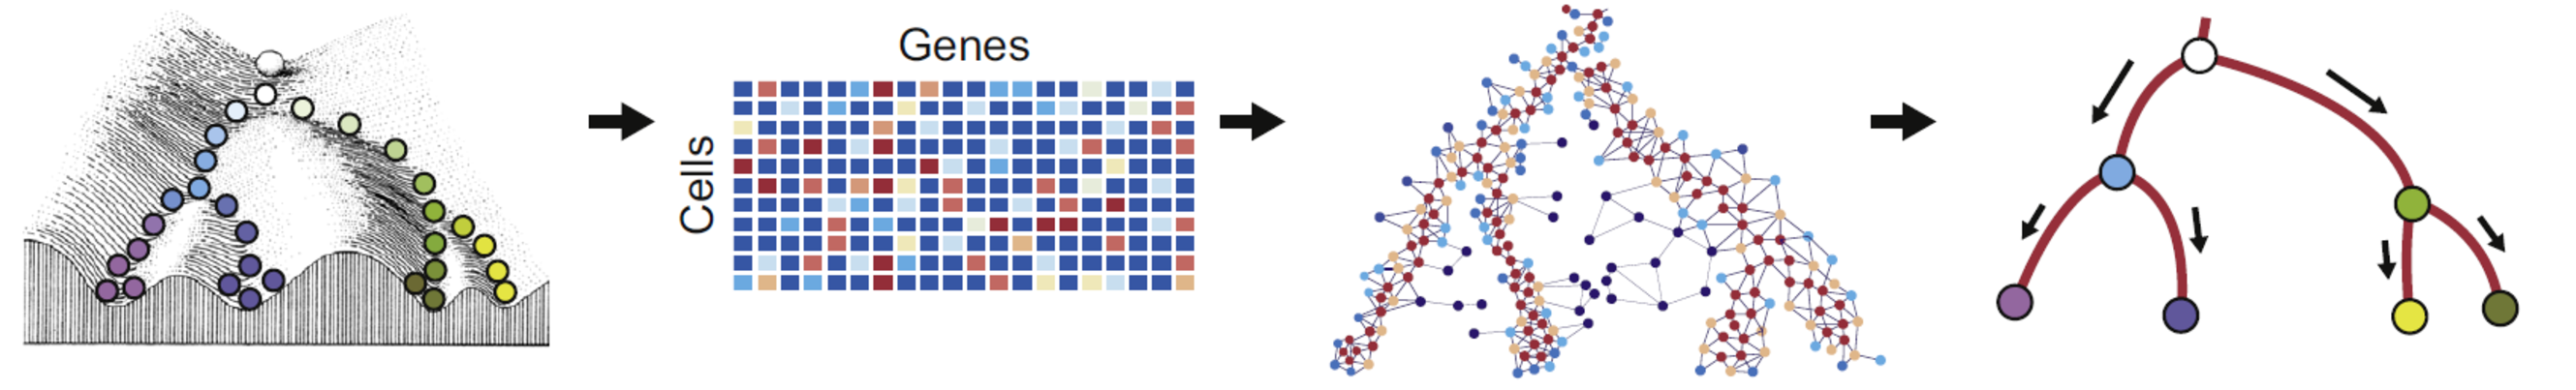
\includegraphics[scale=0.25]{figures/manifold.pdf}
     \caption{\small Intuition of manifolds and geometry underlying sc-data -- {\tiny source: F. Picard}}
   \end{figure}

\end{frame}

% \begin{frame}
%   \frametitle{PCA (and linear methods) limitations}
% 
%   \begin{block}{Do not account for 'complex' data distribution}
%     \begin{itemize}
%       \item PCA is tied to a hidden \alert{\bf Gaussian assumption}
%       \item Fails with \alert{\bf Count data}
%       \item Fails with \alert{\bf Skew data}
%     \end{itemize}
%   \end{block}
%   
%   \vfill
%   
%   \begin{block}{Possible solutions}
%     \begin{itemize}
%       \item Probabilistic (non Gaussian) models
%       \item Need transformed (non-linear) input space
%     \end{itemize}
%   \end{block}
%   
%   \end{frame}

\begin{frame}
  \frametitle{Dimension reduction: revisiting the problem setup}

    \begin{block}{Settings}
      \begin{itemize}
        \item \alert{Training data} : $\mathcal{D}=\{\bx_1,\ldots,\bx_n\} \in \Rset^p$,   (i.i.d.)
        \item Space $\Rset^p$ of possibly high dimension $(n \ll p)$
      \end{itemize}
    \end{block}

    \vfill
    
    \begin{block}{Dimension Reduction Map}
       Construct a map $\Phi$ from the space $\Rset^{p}$ into a space $\Rset^{q}$ of \alert{smaller dimension}:
      \begin{align*}
          \Phi:\quad & \Rset^p \to \Rset^{q}, q \ll p\\
                     & \bx \mapsto \Phi(\bx)
      \end{align*}
    \end{block}
    
\end{frame}

\begin{frame}
  \frametitle{How should we design/construct $\Phi$?}

  \paragraph{Geometrical approach} (\alert{\bf see slides on PCA})
  
  \vfill
  
  \paragraph{Idea to go beyond linear approaches}
  \begin{itemize}
    \item Modify the model by amending the \alert{\bf reconstruction error}
    \item Focus on \alert{\bf Relationship preservation}
  \end{itemize}

  \vfill
  
  \paragraph{Form of the map $\Phi$}
  \begin{itemize}
    \item  Linear or \alert{\bf non-linear ?}
    \item tradeoff between  interpretability and \alert{\bf versatility ?}
    \item tradeoff between  \alert{\bf high} or low computational resource
  \end{itemize}

\end{frame}




\section{Motivated by reconstruction error}

\subsection{PCA as a matrix factorization}

\begin{frame}
  \frametitle{Reconstruction error approach}

  \begin{enumerate}
    \item  Construct a map $\Phi$ from the space $\Rset^{p}$ into a space $\Rset^{q}$ of \alert{smaller dimension}:
      \begin{align*}
      \Phi:\quad & \Rset^{p} \to \Rset^{q}, q \ll p\\
               & \bx \mapsto \Phi(\bx) = \tilde\bx
      \end{align*}
    \item Construct $\tilde{\Phi}$ from $\Rset^{q}$ to $\Rset^{p}$ (\alert{reconstruction formula})
     \item Control an error $\epsilon$ between $\bx$ and its reconstruction $\hat \bx = \tilde{\Phi}(\Phi(\bx))$
  \end{enumerate}

\bigskip

\onslide<2>{
    For instance,  the error measured with the Frobenius between the original data matrix $\bX$ and its approximation:
      \begin{equation*}
        \epsilon(\bX, \hat \bX ) = \left\| \bX - \hat \bX \right\|_F^2  = \sum_{i=1}^n \left\| \bx_i - \tilde{\Phi}(\Phi(\bx_i)) \right\|^2 
      \end{equation*}
}      
\end{frame}

\begin{frame}
\frametitle{Reinterpretation of PCA}

  \begin{block}{PCA model}
       Let $\bV$ be a $p\times q$ matrix whose columns are of $q$ orthonormal vectors.
      \begin{align*}
        \Phi(\bx) & = \bV^\top(\bx-\bmu)  = \tilde\bx \\  
        \bx \simeq \tilde{\Phi}(\tilde\bx) & = \bmu + \bV \tilde\bx
      \end{align*}
      \rsa Model with \alert{\bf Linear assumption + ortho-normality constraints}
    \end{block}

  \begin{block}{PCA reconstruction error}<2>
    \vspace{-.25cm}
    \begin{equation*}
      \minimize_{\bmu \in\Rset^p, \bV\in\mathcal{O}_{p,q}} \sum_{i=1}^n \left\| (\bx_i  - \bmu) - \bV\bV^\top ( \bx_i -\bmu)   \right\|^2 
    \end{equation*}
  
  \alert{Solution (explicit)} 
  \begin{itemize}
  \item $\bmu = \bar{\bx}$ the empirical mean
  \item $\bV$  an orthonormal basis of the space spanned by the $q$ first eigenvectors of the empirical covariance matrix
  \end{itemize}
  
  \end{block}
\end{frame}

\begin{frame}
  \frametitle{Important digression: SVD}

  \begin{block}{Singular Value Decomposition (SVD)}
    The SVD of $\mathbf{M}$ a $n\times p$ matrix is the factorization given by
    
    \[ \mathbf{M} =\mathbf{U}\mathbf{D}\mathbf{V}^\top,\]
    where $r = \min(n,p)$ and
    \begin{itemize}
      \item \(\mathbf{D}_{r \times r} = \text{diag}(\delta_1, ...\delta_r)\) is the diagonal matrix of singular values.
      \item \(\mathbf{U}\) is orthonormal, whose columns are eigen vectors of (\(\mathbf{M}\mathbf{M}^T\))
      \item \(\mathbf{V}\) is orthonormal whose columns are eigen vectors of (\(\mathbf{M}^T\mathbf{M}\))
    \end{itemize}
    {\small \rsa Time complexity in $\mathcal{O}(n p q r)$ (less when $k\ll r$ components are required)}
  \end{block}

  \vfill
  
  \begin{block}{Connection with eigen decomposition of the covariance matrix}<2>
    \vspace{-.5cm}
    \begin{align*}
      \mathbf{M}^\top\mathbf{M} & = \mathbf{V} \mathbf{D} \mathbf{U}^\top  \mathbf{U} \mathbf{D} \mathbf{V}^\top \\
        & = \mathbf{V} \mathbf{D}^2 \mathbf{V}^\top  = \mathbf{V} \boldsymbol{\Lambda} \mathbf{V}^\top\\
    \end{align*}
  \end{block}

\end{frame}

%%%%%%%%%%%%%%%%%%%%%%%%%%
%%%%%%%%%%%%%%%%%%%%%%%%%%%%
\begin{frame}{PCA solution is given by SVD of the centered data matrix}

\begin{figure}[ht]
  \centering
  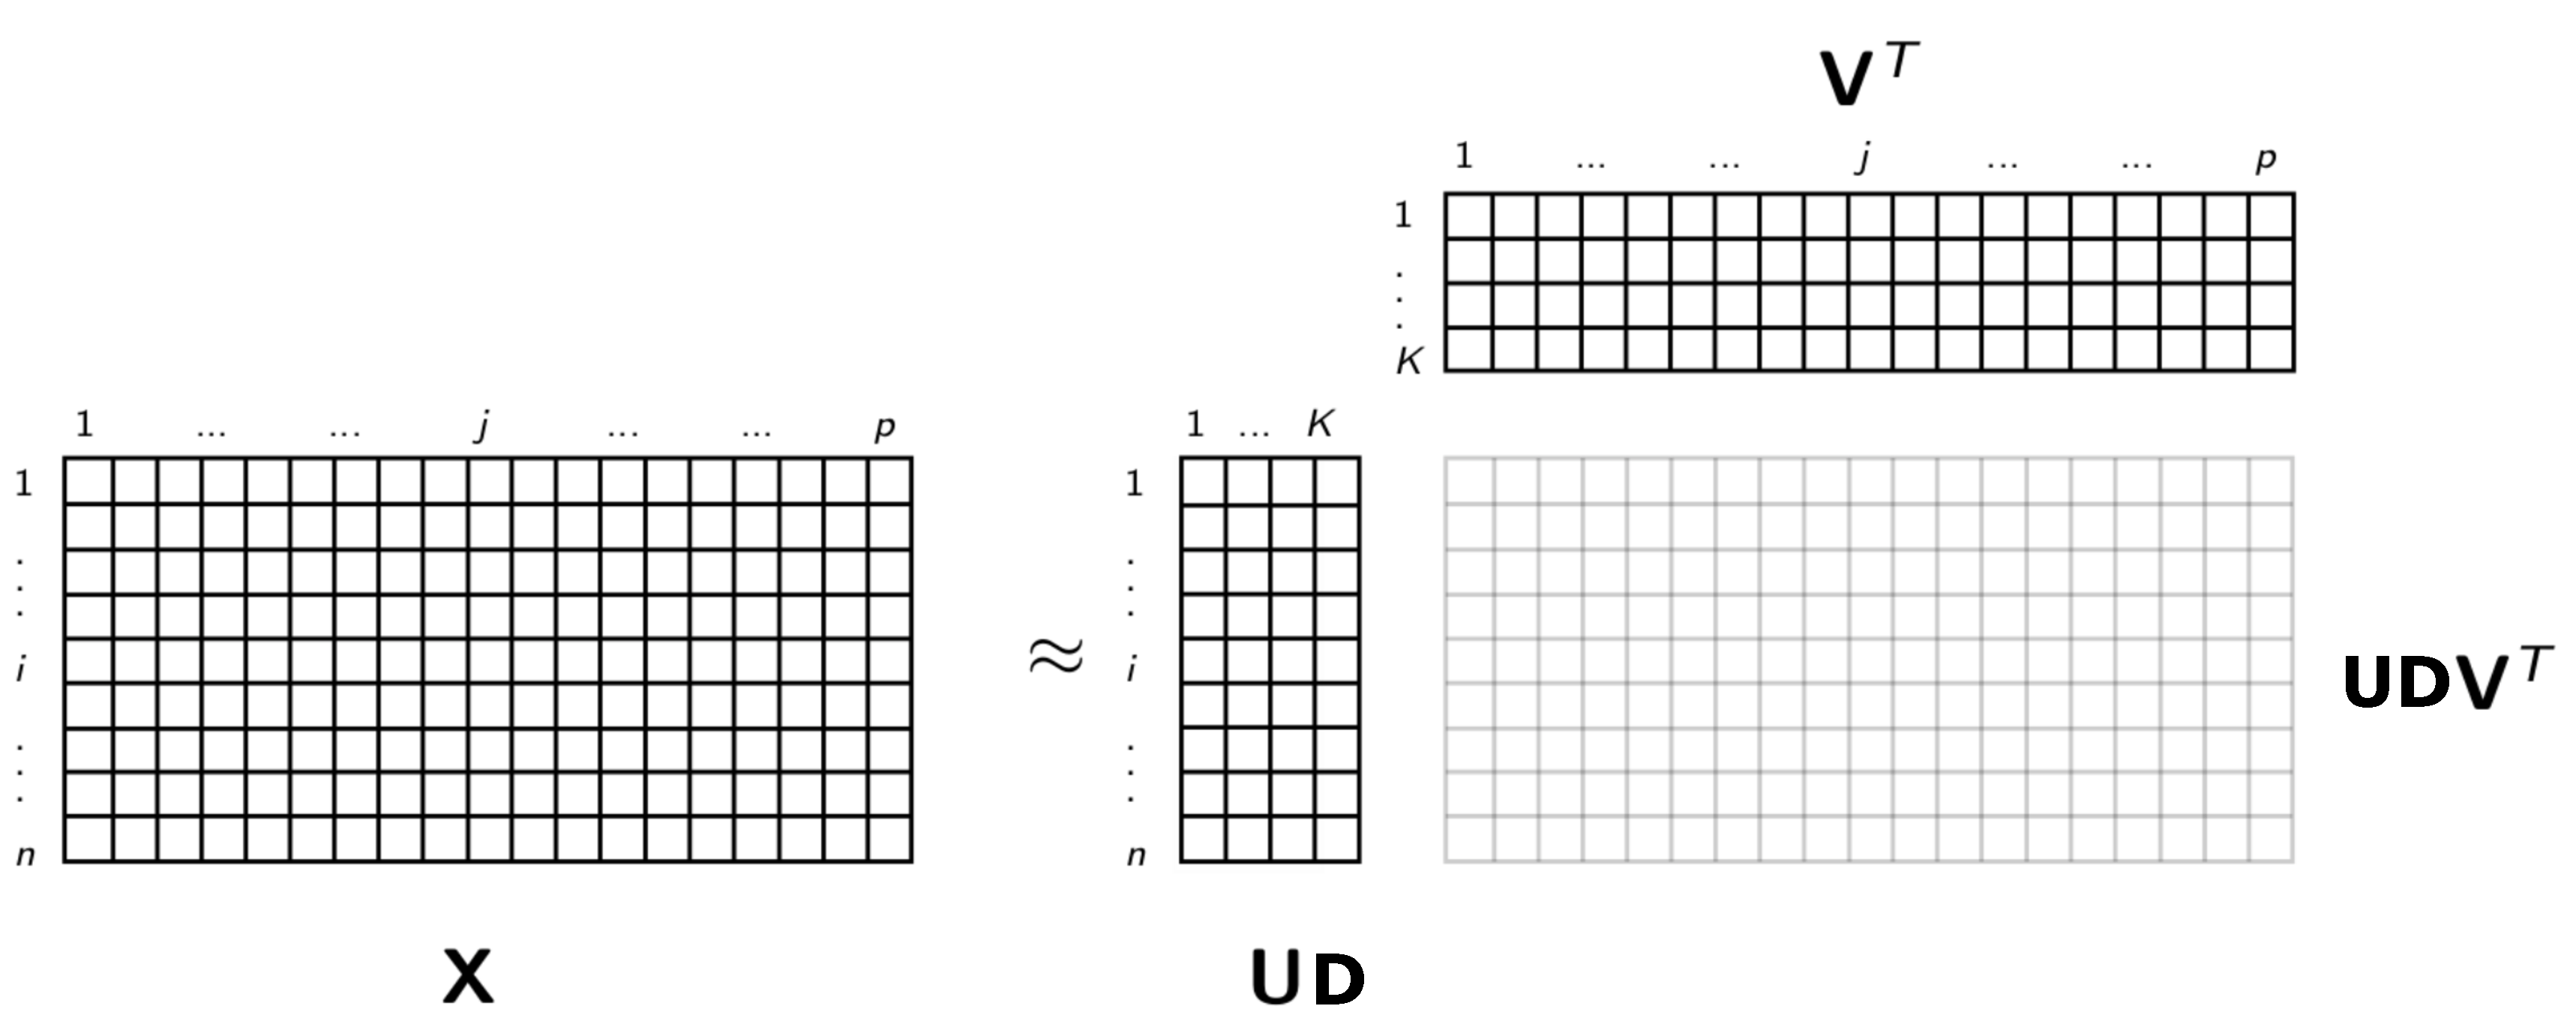
\includegraphics[height=4cm]{figures/matrix_factorization}
\end{figure}

Since $\tilde\bX = \mathbf{\bX}^c \bV =  \bU \bD \bV^\top \bV = \bU \bD$, PCA can be rephrased as
\[ \hat{\mathbf{X}^c} = \mathbf{FV}^\top =  \argmin_{\mathbf{F}\in\mathcal{M}_{n,q},\bV\in\mathcal{O}_{p,q} } \left\| \mathbf{X}^c - \mathbf{FV}^\top \right\|_F^2 \text{ with } \|\mathbf{A}\|_F^2 = \sum_{ij} a_{ij}^2, 
\]
\[
  \left. \tilde\bX \in\Rset^{n\times \textcolor{red}{q}}, \mathbf{V}\in\Rset^{p\times \textcolor{red}{q}} \right\} \ \text{Best linear low-rank representation of $\bX$}
\]

\end{frame}
 

\subsection{Kernel-PCA}



\begin{frame}
  \frametitle{Kernel-PCA}
  
  \begin{block}{Principle: non linear transformation of $\bx$ prior to linear PCA} 
    \begin{enumerate}
      \item Project the data into a higher space where it is linearly separable
      \item Apply PCA to the transformed data 
    \end{enumerate}
  \end{block}

  \begin{figure}[ht]
    \centering
    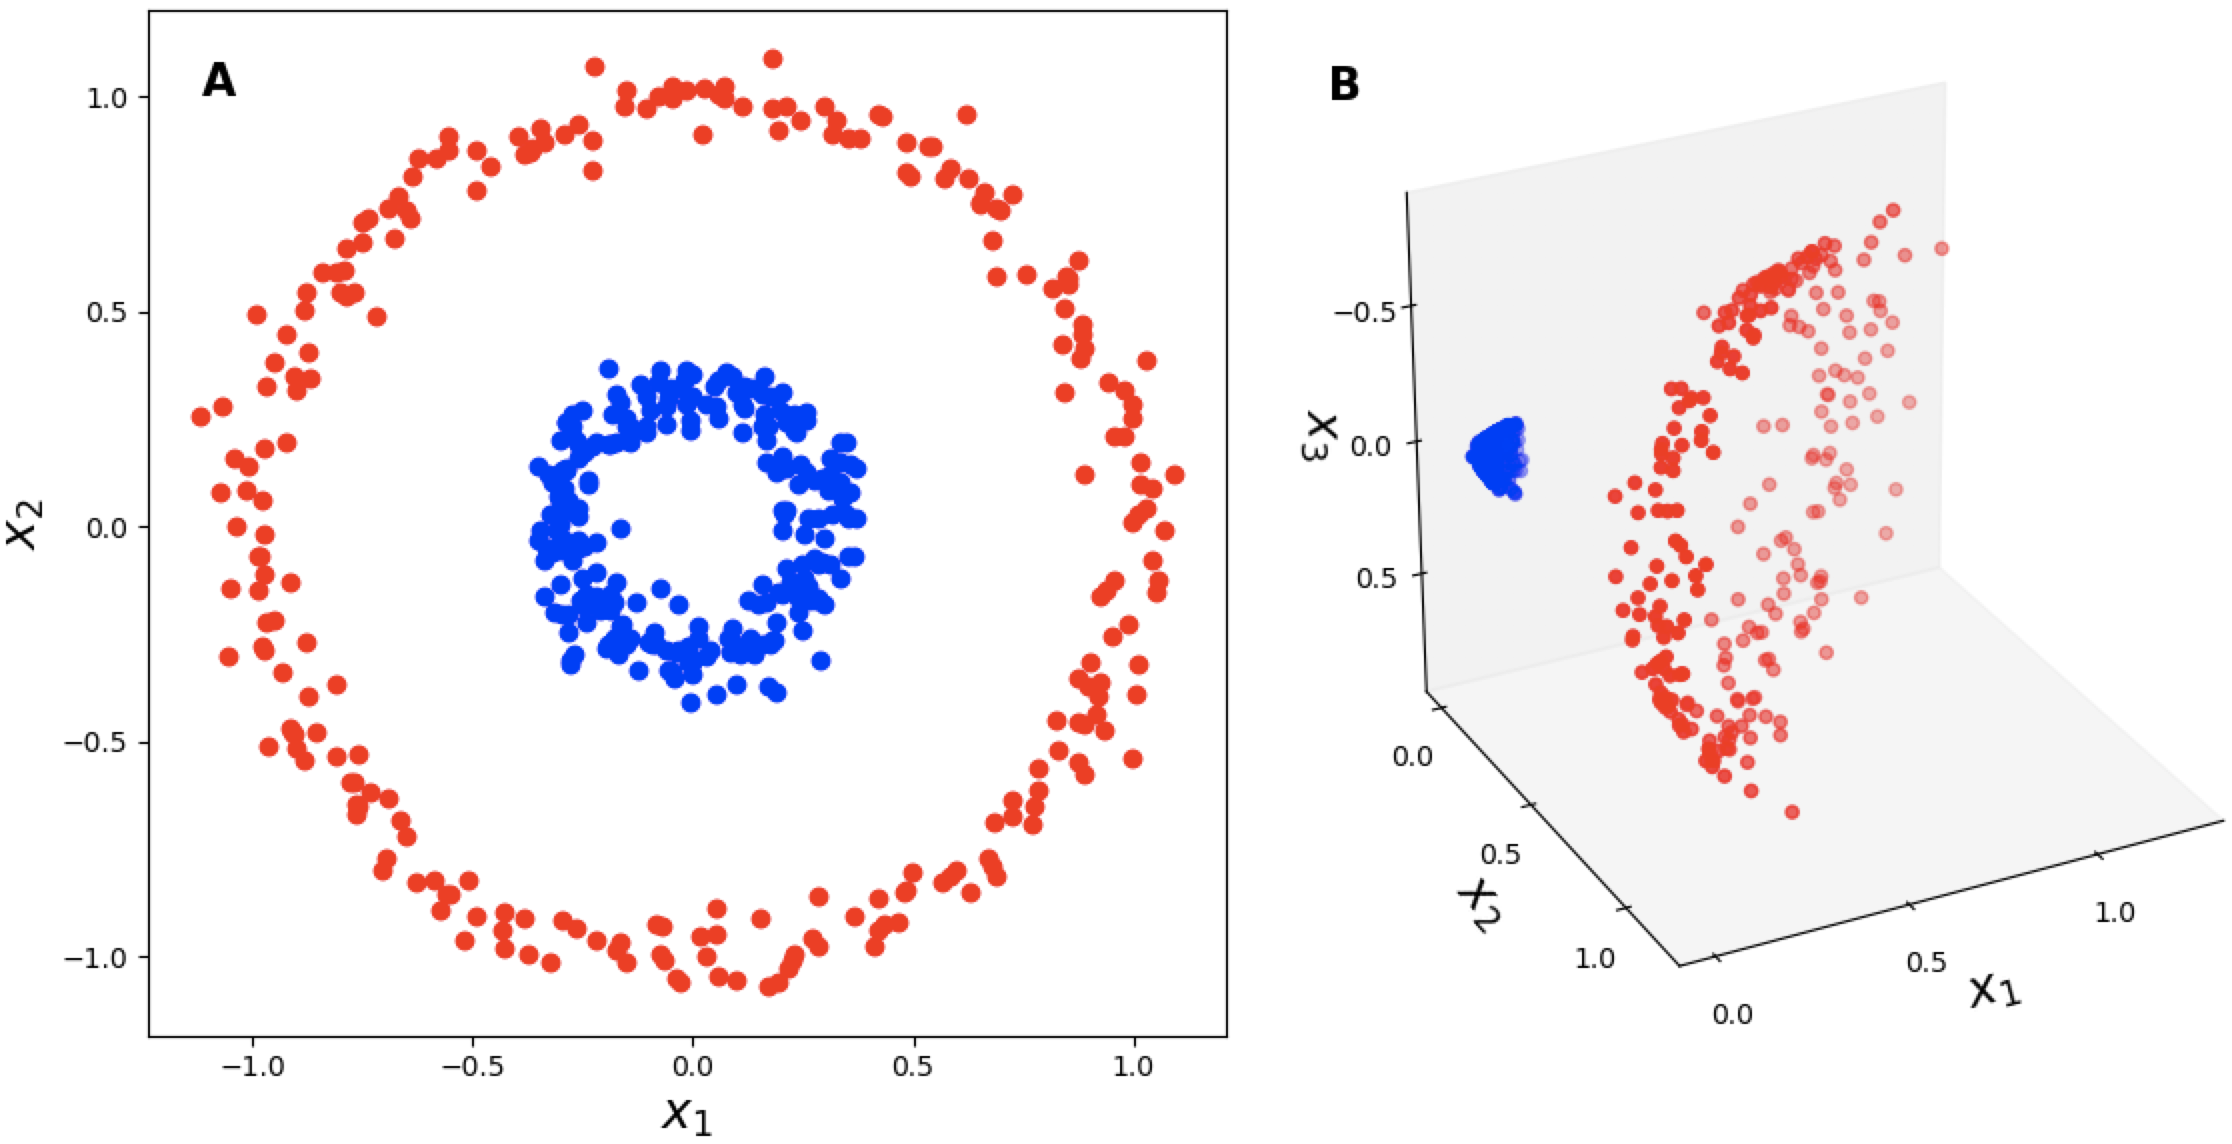
\includegraphics[height=4cm]{figures/kernel_trick2}
    \caption{Transformation $\Psi : \bx \to \Psi(\bx)$ (illustration in presence of existing labels)}
  \end{figure}

\end{frame}

\begin{frame}
  \frametitle{Kernel-PCA}

  \begin{block}{Kernel PCA Model}
    Assume a non linear transformation $ \Psi(\mathbf{x}_i) \text{ where } \Psi : \mathbb{R}^p \to \mathbb{R}^n$,  then perform linear PCA, with $\bV$ a \alert{\bf $n\times q$} orthonormal matrix
    \[
      \Phi(\bx) = \bV^\top \Psi(\bx-\bmu) = \tilde\bx
    \]
  \end{block}

  \begin{block}{Kernel trick}
    Never calculate  $\Psi(\bx_i)$ thanks to the kernel trick:
    \[K = k(\mathbf{x},\mathbf{y}) = (\Psi(\mathbf{x}),\Psi(\mathbf{y})) = \Psi(\mathbf{x})^T\Psi(\mathbf{y}) \]
  \end{block}

  \begin{block}{Solution}
    Eigen-decomposition of the doubly centered kernel matrix $\mathbf{K} = k(\bx_i, \bx_{i'})$ 
    \[\tilde{\mathbf{K}} = 
    (\bI - \mathbf{1}\mathbf{1}^\top/n) \mathbf{K} (\bI - \mathbf{1}\mathbf{1}^\top/n) = \bV {\boldsymbol\Lambda} \bV^\top \]
  \end{block}

\end{frame}

\begin{frame}[fragile]
  \frametitle{Choice of a kernel} 

  A symmetric positive definite function $k(\mathbf{x},\mathbf{y}) \in \Rset$, which depends on the kind of \alert{\bf similarity} assumed

\begin{block}{Some common kernels}

\begin{itemize}
\item \alert{\bf Polynomial Kernel }

\[ k(\bx_i,\bx_{i'}) = (\bx_{i}^\top \bx_{i'} + c)^d \]

\item  \alert{\bf Gaussian (radial) kernel}

\[k(\bx_i,\bx_{i'}) = \exp{\frac {-\left\|\bx_i - \bx_{i'} \right\|^2}{2\sigma^2}}\]

\item  \alert{\bf Laplacian kernel}

\[k(\bx_i,\bx_{i'}) = \exp{\frac {-\left\|\bx_i - \bx_{i'} \right\|}{\sigma}}\]

\end{itemize}
\end{block}

\rsa Kernel PCA suffers from the choice of the Kernel

\end{frame}


\begin{frame}[fragile]
  \frametitle{Example on scRNA} 
  \framesubtitle{Run the fit}

\begin{knitrout}\scriptsize
\definecolor{shadecolor}{rgb}{0.969, 0.969, 0.969}\color{fgcolor}\begin{kframe}
\begin{alltt}
\hlstd{scRNA_expr} \hlkwb{<-} \hlstd{scRNA} \hlopt \hlstd{dplyr}\hlopt{::}\hlkwd{select}\hlstd{(}\hlopt{-}\hlstd{cell_type)} \hlopt \hlkwd{as.matrix}\hlstd{()}

\hlstd{kPCA_radial} \hlkwb{<-}
  \hlkwd{kpca}\hlstd{(scRNA_expr,} \hlkwc{kernel} \hlstd{=} \hlstr{"rbfdot"}\hlstd{,} \hlkwc{features} \hlstd{=} \hlnum{2}\hlstd{,} \hlkwc{kpar} \hlstd{=} \hlkwd{list}\hlstd{(}\hlkwc{sigma} \hlstd{=} \hlnum{0.5}\hlstd{))} \hlopt
  \hlkwd{pcv}\hlstd{()} \hlopt \hlkwd{as.data.frame}\hlstd{()} \hlopt
  \hlkwd{add_column}\hlstd{(}\hlkwc{kernel} \hlstd{=} \hlstr{"Radial"}\hlstd{)} \hlopt
  \hlkwd{add_column}\hlstd{(}\hlkwc{cell_type} \hlstd{= scRNA}\hlopt{$}\hlstd{cell_type)}

\hlstd{kPCA_linear} \hlkwb{<-}
  \hlkwd{kpca}\hlstd{(scRNA_expr,} \hlkwc{kernel} \hlstd{=} \hlstr{"vanilladot"}\hlstd{,} \hlkwc{features} \hlstd{=} \hlnum{2}\hlstd{,} \hlkwc{kpar} \hlstd{=} \hlkwd{list}\hlstd{())} \hlopt
  \hlkwd{pcv}\hlstd{()} \hlopt \hlkwd{as.data.frame}\hlstd{()} \hlopt
  \hlkwd{add_column}\hlstd{(}\hlkwc{kernel} \hlstd{=} \hlstr{"Linear"}\hlstd{)} \hlopt
  \hlkwd{add_column}\hlstd{(}\hlkwc{cell_type} \hlstd{= scRNA}\hlopt{$}\hlstd{cell_type)}

\hlstd{kPCA_polydot} \hlkwb{<-} \hlkwd{kpca}\hlstd{(scRNA_expr,} \hlkwc{kernel} \hlstd{=} \hlstr{"polydot"}\hlstd{,} \hlkwc{features} \hlstd{=} \hlnum{2}\hlstd{,} \hlkwc{kpar} \hlstd{=} \hlkwd{list}\hlstd{(}\hlkwc{degree} \hlstd{=} \hlnum{3}\hlstd{))} \hlopt
  \hlkwd{pcv}\hlstd{()} \hlopt \hlkwd{as.data.frame}\hlstd{()} \hlopt
  \hlkwd{add_column}\hlstd{(}\hlkwc{kernel} \hlstd{=} \hlstr{"Polynomial"}\hlstd{)} \hlopt
  \hlkwd{add_column}\hlstd{(}\hlkwc{cell_type} \hlstd{= scRNA}\hlopt{$}\hlstd{cell_type)}

\hlstd{kPCA_laplacedot} \hlkwb{<-} \hlkwd{kpca}\hlstd{(scRNA_expr,} \hlkwc{kernel} \hlstd{=} \hlstr{"laplacedot"}\hlstd{,} \hlkwc{features} \hlstd{=} \hlnum{2}\hlstd{)} \hlopt
  \hlkwd{pcv}\hlstd{()} \hlopt \hlkwd{as.data.frame}\hlstd{()} \hlopt
  \hlkwd{add_column}\hlstd{(}\hlkwc{kernel} \hlstd{=} \hlstr{"Laplace"}\hlstd{)} \hlopt
  \hlkwd{add_column}\hlstd{(}\hlkwc{cell_type} \hlstd{= scRNA}\hlopt{$}\hlstd{cell_type)}
\end{alltt}
\end{kframe}
\end{knitrout}
\end{frame}

\begin{frame}[fragile]
  \frametitle{Example on scRNA} 
  \framesubtitle{Compare the projections}

\begin{knitrout}\scriptsize
\definecolor{shadecolor}{rgb}{0.969, 0.969, 0.969}\color{fgcolor}\begin{kframe}
\begin{alltt}
\hlkwd{rbind}\hlstd{(kPCA_linear, kPCA_polydot, kPCA_radial, kPCA_laplacedot)} \hlopt
  \hlkwd{ggplot}\hlstd{(}\hlkwd{aes}\hlstd{(}\hlkwc{x} \hlstd{= V1,} \hlkwc{y} \hlstd{= V2,} \hlkwc{color} \hlstd{= cell_type))} \hlopt{+}
  \hlkwd{geom_point}\hlstd{(}\hlkwc{size}\hlstd{=}\hlnum{1.25}\hlstd{)} \hlopt{+} \hlkwd{guides}\hlstd{(}\hlkwc{colour} \hlstd{=} \hlkwd{guide_legend}\hlstd{(}\hlkwc{override.aes} \hlstd{=} \hlkwd{list}\hlstd{(}\hlkwc{size}\hlstd{=}\hlnum{6}\hlstd{)))} \hlopt{+}
  \hlkwd{facet_wrap}\hlstd{(.}\hlopt{~}\hlstd{kernel,} \hlkwc{scales} \hlstd{=} \hlstr{'free'}\hlstd{)} \hlopt{+} \hlkwd{labs}\hlstd{(}\hlkwc{x} \hlstd{=} \hlstr{''}\hlstd{,} \hlkwc{y} \hlstd{=} \hlstr{''}\hlstd{)}
\end{alltt}
\end{kframe}
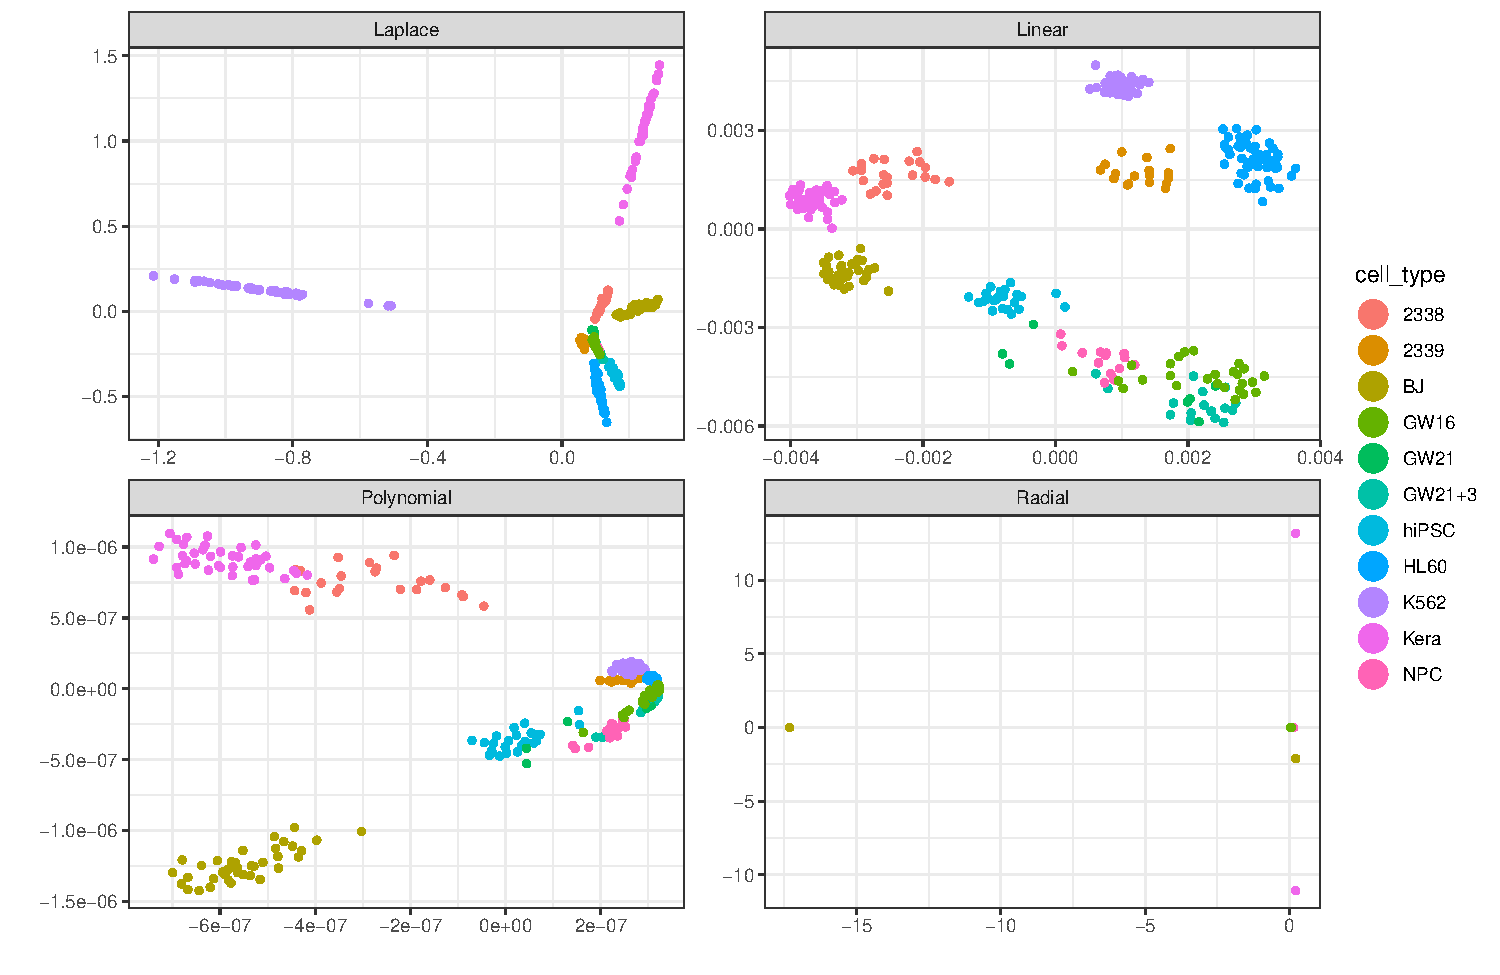
\includegraphics[width=.8\textwidth]{figures/kPCA_scRNA_kernel_plot-1} 
\end{knitrout}

\end{frame}


\subsection{Other directions}

\begin{frame}
  \frametitle{Other approaches}
  \framesubtitle{Linear model with other constraints}
    
    Let $\bV$ be a $p\times q$ matrix and $\tilde \bx \in \Rset^q$
    \begin{equation*}
      \bx \simeq  \bmu + \sum_{j=1}^q \tilde x^j \bV^j = \bmu + \bV \tilde\bx
    \end{equation*}
  
    Apply other constraints on $\bV$ and or the factor/representation $\tilde\bx$
    \begin{itemize}
      \item $\bV$ and $\tilde\bx$ non-negative: \alert{\bf Non-negative Matrix Factorization}\\
\begin{knitrout}\scriptsize
\definecolor{shadecolor}{rgb}{0.969, 0.969, 0.969}\color{fgcolor}\begin{kframe}
\begin{alltt}
\hlkwd{library}\hlstd{(NMF)}
\end{alltt}
\end{kframe}
\end{knitrout}
      \item $\bV$ sparse, possibly orthogonal: \alert{\bf sparse PCA}\\
\begin{knitrout}\scriptsize
\definecolor{shadecolor}{rgb}{0.969, 0.969, 0.969}\color{fgcolor}\begin{kframe}
\begin{alltt}
\hlkwd{library}\hlstd{(sparsepca)}
\end{alltt}
\end{kframe}
\end{knitrout}
      \item $\tilde \bx$ sparse : \alert{\bf Dictionary learning}
\begin{knitrout}\scriptsize
\definecolor{shadecolor}{rgb}{0.969, 0.969, 0.969}\color{fgcolor}\begin{kframe}
\begin{alltt}
\hlkwd{library}\hlstd{(SPAMS)}
\end{alltt}
\end{kframe}
\end{knitrout}
      \item ($\tilde X^j, \tilde X^\ell$) independent : \alert{\bf Independent Component Anaysis}
\begin{knitrout}\scriptsize
\definecolor{shadecolor}{rgb}{0.969, 0.969, 0.969}\color{fgcolor}\begin{kframe}
\begin{alltt}
\hlkwd{library}\hlstd{(fastICA)}
\end{alltt}
\end{kframe}
\end{knitrout}
    \end{itemize}

\end{frame}
 
\begin{frame}
   \frametitle{Auto-encoders}
   
   \begin{block}{Highly non-linear model}

      Find $\Phi$ and $\tilde\Phi$ with \alert{\bf two} neural-networks, controlling the error.

      \begin{equation*}
        \epsilon(\bX, \hat \bX ) = \sum_{i=1}^n \left\| \bx_i - \tilde{\Phi}(\Phi(\bx_i)) \right\|^2 \alert{\bf + \text{regularization}(\Phi, \tilde\Phi)}
      \end{equation*}

      \begin{itemize}
         \item \# layers and neurons determine the \alert{\bf model complexity}
         \item Need regularization to avoid \alert{\bf overfitting}
         \item  Fitted with optimization tools like stochastic gradient descent
         \item Require much \alert{more data} and more computational \alert{resources}
         \item \alert{\bf Interpretation questionable}
      \end{itemize}

   \end{block}

Some Python equivalents of (torch, pytorch, tensorflow):
 
\begin{knitrout}\scriptsize
\definecolor{shadecolor}{rgb}{0.969, 0.969, 0.969}\color{fgcolor}\begin{kframe}
\begin{alltt}
\hlkwd{library}\hlstd{(keras)}

\hlkwd{library}\hlstd{(torch)}
\end{alltt}
\end{kframe}
\end{knitrout}

\end{frame}


%% ==========================================================================
\section{Motivated by relation preservation}
%% ==========================================================================


\begin{frame}
    \frametitle{Pairwise Relation}

    Focus on pairwise relation $\mathcal{R}(\bx_i, \bx_{i'})$.

    \begin{block}{Distance Preservation}
      \begin{itemize}
    \item  Construct a map $\Phi$ from the space $\Rset^{p}$ into a space $\Rset^{q}$ of \alert{smaller dimension}:
      \begin{align*}
      \Phi:\quad & \Rset^p \to \Rset^{q}, q \ll p\\
               & \bx \mapsto \Phi(\bx)
      \end{align*}
      \begin{equation*}
      \text{such that} \quad \mathcal{R}(\bx_i, \bx_{i'}) \sim\mathcal{R'}(\tilde\bx_i, \tilde\bx_{i'})
      \end{equation*}
    \end{itemize}
  \end{block}

  \begin{block}{Multidimensional scaling}
    Try to preserve inner product related to the distance (e.g. Euclidean)
  \end{block}

  \vfill

  \begin{block}{t-SNE -- Stochastic Neighborhood Embedding}
    Try to preserve relations with close neighbors with Gaussian kernel
  \end{block}

\end{frame}


\subsection{Stochastic Neighborhood Embedding}



\begin{frame}{Stochastic Neighbor Embedding (SNE)}

Let $(\bx_1, \hdots, \bx_n)$ be the original points in $\mathbb{R}^p$, and measure similarities by

\[p_{ij} =  (p_{j | {i}} + p_{{i} | j})/ 2n\]
where
\begin{align*}
  p_{j | {i}} & = \frac{ \exp(- \| \bx_j - \bx_{i} \|^2 / 2 \sigma_i^2 ) }{\sum_{k \neq i} \exp(- \| \bx_k - \bx_{i} \|^2 / 2 \sigma_{i}^2)}, \\
  & = \frac{ \exp(- d_{ij}^2 / 2 \sigma_i^2 ) }{\sum_{k \neq i} \exp(- d_{ki}^2 / 2 \sigma_i^2)}
\end{align*}

\vfill

\begin{itemize}
\item[\rsa] SNE preserves relations with \alert{\bf close neighbors} with Gaussian kernels
\item[\rsa] $\sigma$ smooths the data (linked to the regularity of the target manifold)
\end{itemize}

\end{frame}

\begin{frame}{The perplexity parameter}

The variance $\sigma_i^2$ should adjust to local densities (neighborhood of point $i$)

\begin{block}{Perplexity: a smoothed effective number of neighbors}
The perplexity is defined by
$$
  Perp(p_i) = 2^{H(p_i)}, \qquad H(p_i) = -\sum_{j=1}^{n} p_{j|i} \log_2 p_{j|i}
$$
where $H$ is the Shannon entropy of $p_i=(p_{1|i},\hdots,p_{n|i})$.\\
\end{block}

\vfill

\rsa SNE performs a binary search for the value of $\sigma_i$ that produces a $p_i$ with a fixed perplexity that is specified by the user.

\end{frame}

\begin{frame}{tSNE and Student / Cauchy kernels}

Consider $(\tilde\bx_1,\hdots,\tilde\bx_n)$ are points in the low dimensional space $\mathbb{R}^{q=2}$

\begin{itemize}
\item Consider a similarity between points in the new representation:
$$q_{i | j} = \frac{ \exp(- \| \tilde\bx_i - \tilde\bx_j \|^2  ) }{\sum_{k \neq i} \exp(- \| \tilde\bx_k - \tilde\bx_j \|^2 )}$$
\item Robustify this kernel by using Student(1) kernels (ie Cauchy)
$$q_{i | j} = \frac{ (1 + \| \tilde\bx_i - \tilde\bx_j \|^2)^{-1}  }{\sum_{k \neq i} (1 + \| \tilde\bx_i - \tilde\bx_k \|^2)^{-1}}$$
\end{itemize}
\end{frame}

% \begin{frame}{Optimizing tSNE}
% \begin{itemize}
% \item Minimize the KL between $p$ and $q$ so that the data representation minimizes:
% $$
% C(y) = \sum_{ij} KL(p_{ij},q_{ij})
% $$
% \item The cost function is not convex 
% $$
% \left[ \frac{\partial C(y)}{\partial y} \right]_i = \sum_{j} (p_{ij}-q_{ij})(y_i - y_j)
% $$
% \item Interpreted as the resultant force created by a set of springs between the map point $y_i$ and all other map points $\left( y_j \right)_j$. All springs exert a force along the direction $(y_i - y_j)$.
% \item $(p_{ij}-q_{ij})$ is viewed as a stiffness of the force exerted by the spring between $y_i$ and $y_j$.
% \end{itemize}
% \end{frame}

% \begin{frame}{Customed Gradient descent}
% \begin{itemize}
% \item Gradient descent initialized by sampling map points randomly from an isotropic Gaussian with small variance centered around the origin
% \item Gradient update using
% $$
% y^{(t)} = y^{(t-1)} + \eta \frac{\partial C(y)}{\partial y} + \alpha(t) (y^{(t-1)}-y^{(t-2)})
% $$
% \item $\eta$ learning rate, $\alpha(t)$ momentum at iteration $t$.
% \item Gaussian noise is added to the map points to perform simulated annealing.
% \end{itemize}
% \end{frame}

\begin{frame}{t-SNE: pros/cons}

\begin{block}{Properties}
\begin{itemize}
\item good at preserving local distances (intra-cluster variance)
\item not so good for global representation (inter-cluster variance)
\item good at creating clusters of close points, bad at positioning clusters wrt each other
\end{itemize}
\end{block}

\begin{block}{Limitations}
\begin{itemize}
  \item importance of preprocessing: initialize with PCA and feature selection plus log transform (non linear transform)
\item percent of explained variance ? interpretation of the $q$ distribution ?
\end{itemize}
\end{block}

\end{frame}

\begin{frame}[fragile,allowframebreaks]
  \frametitle{Example on scRNA} 

\paragraph{Run the fit}

\begin{knitrout}\scriptsize
\definecolor{shadecolor}{rgb}{0.969, 0.969, 0.969}\color{fgcolor}\begin{kframe}
\begin{alltt}
\hlstd{scRNA_expr} \hlkwb{<-} \hlstd{scRNA} \hlopt \hlstd{dplyr}\hlopt{::}\hlkwd{select}\hlstd{(}\hlopt{-}\hlstd{cell_type)} \hlopt \hlkwd{as.matrix}\hlstd{()}

\hlstd{tSNE_perp2}   \hlkwb{<-} \hlkwd{Rtsne}\hlstd{(scRNA_expr,} \hlkwc{perplexity} \hlstd{=}   \hlnum{2}\hlstd{)}\hlopt{$}\hlstd{Y} \hlopt
  \hlkwd{as.data.frame}\hlstd{()} \hlopt \hlkwd{add_column}\hlstd{(}\hlkwc{perplexity} \hlstd{=} \hlnum{2}\hlstd{)} \hlopt \hlkwd{add_column}\hlstd{(}\hlkwc{cell_type} \hlstd{= scRNA}\hlopt{$}\hlstd{cell_type)}

\hlstd{tSNE_perp10}  \hlkwb{<-} \hlkwd{Rtsne}\hlstd{(scRNA_expr,} \hlkwc{perplexity} \hlstd{=}  \hlnum{10}\hlstd{)}\hlopt{$}\hlstd{Y} \hlopt
  \hlkwd{as.data.frame}\hlstd{()} \hlopt \hlkwd{add_column}\hlstd{(}\hlkwc{perplexity} \hlstd{=} \hlnum{10}\hlstd{)} \hlopt \hlkwd{add_column}\hlstd{(}\hlkwc{cell_type} \hlstd{= scRNA}\hlopt{$}\hlstd{cell_type)}

\hlstd{tSNE_perp100} \hlkwb{<-} \hlkwd{Rtsne}\hlstd{(scRNA_expr,} \hlkwc{perplexity} \hlstd{=} \hlnum{100}\hlstd{)}\hlopt{$}\hlstd{Y} \hlopt
  \hlkwd{as.data.frame}\hlstd{()} \hlopt \hlkwd{add_column}\hlstd{(}\hlkwc{perplexity} \hlstd{=} \hlnum{100}\hlstd{)} \hlopt \hlkwd{add_column}\hlstd{(}\hlkwc{cell_type} \hlstd{= scRNA}\hlopt{$}\hlstd{cell_type)}
\end{alltt}
\end{kframe}
\end{knitrout}

\paragraph{Compare perplexity}

\begin{knitrout}\scriptsize
\definecolor{shadecolor}{rgb}{0.969, 0.969, 0.969}\color{fgcolor}\begin{kframe}
\begin{alltt}
\hlkwd{rbind}\hlstd{(tSNE_perp2,tSNE_perp10,tSNE_perp100)} \hlopt
  \hlkwd{ggplot}\hlstd{(}\hlkwd{aes}\hlstd{(}\hlkwc{x} \hlstd{= V1,} \hlkwc{y} \hlstd{= V2,} \hlkwc{color} \hlstd{= cell_type))} \hlopt{+}
     \hlkwd{geom_point}\hlstd{(}\hlkwc{size}\hlstd{=}\hlnum{1.25}\hlstd{)} \hlopt{+}
     \hlkwd{guides}\hlstd{(}\hlkwc{colour} \hlstd{=} \hlkwd{guide_legend}\hlstd{(}\hlkwc{override.aes} \hlstd{=} \hlkwd{list}\hlstd{(}\hlkwc{size}\hlstd{=}\hlnum{6}\hlstd{)))} \hlopt{+}
  \hlkwd{facet_wrap}\hlstd{(.}\hlopt{~}\hlstd{perplexity,} \hlkwc{scales} \hlstd{=} \hlstr{'free'}\hlstd{)}
\end{alltt}
\end{kframe}
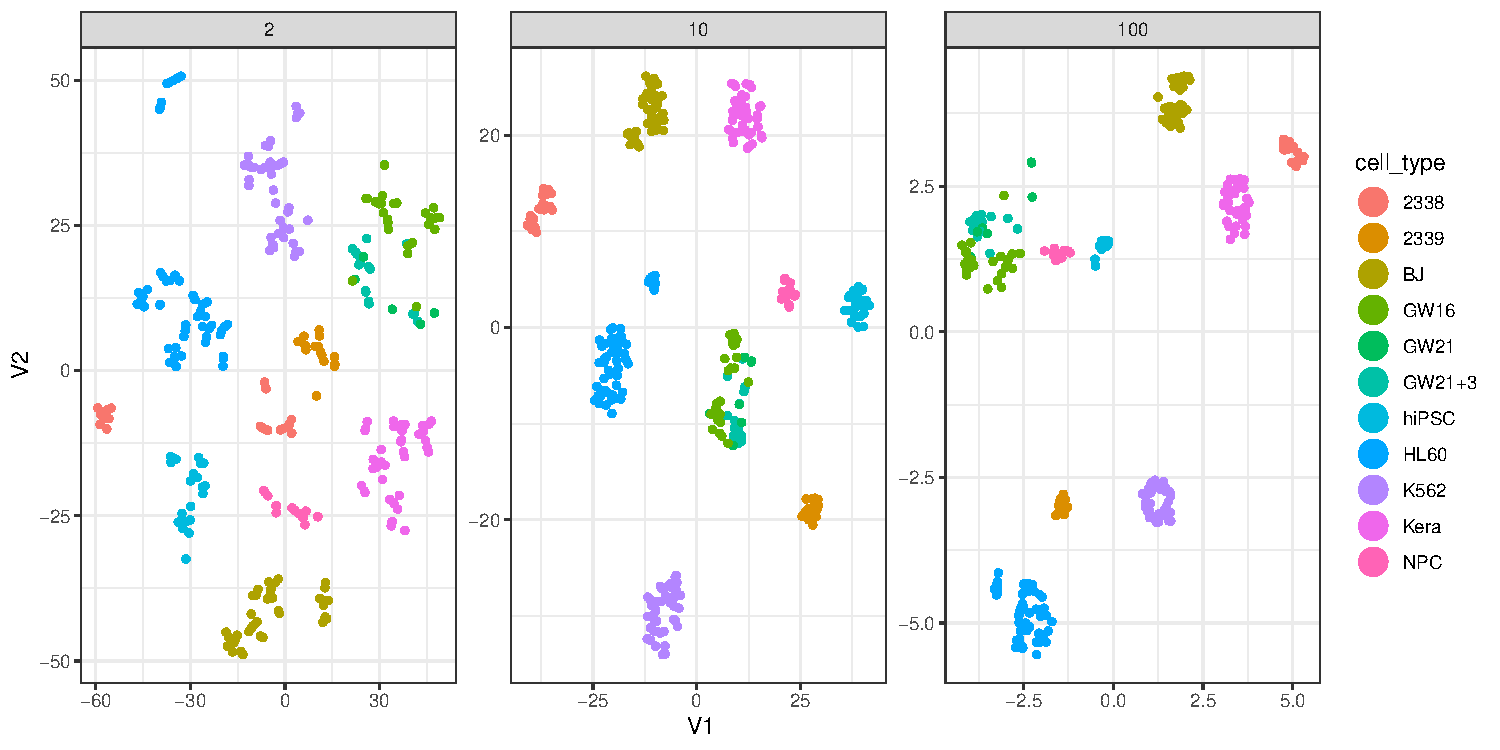
\includegraphics[width=\textwidth]{figures/tSNE_scRNA_perplexity_plot-1} 
\end{knitrout}

\end{frame}


\subsection{Other methods}



\begin{frame}{Multidimensional scaling}
  \framesubtitle{a.k.a Principale Coordinates Analysis}

  \begin{block}{Problem setup}
  Consider a collection of points $\bx_i\in\Rset^p$ and assume either 
  \begin{itemize}
  \item $D = d_{ii'}$ a $n\times n$ dissimilarity matrix, or
  \item $S = s_{ii'}$ a $n\times n$ similarity matrix, or
  \end{itemize}
  \alert{Goal:} find $\tilde\bx_i\in\Rset^q$ while preserving S/D in the latent space\\
  \end{block}
  
  \rsa Don't need access to the position in $\Rset^p$ (only $D$ or $S$ \rsa 'kernel').


  \begin{block}{Classical MDS model}
    Measure similarities with the (centered) \alert{\bf inner product} and minimize 
    \begin{equation*}
      \sum_{i\neq i'} \left( (\bx_i - \bmu)^\top (\bx_i - \bmu) - \tilde\bx_i^\top \tilde\bx_{i'} \right)^2,
    \end{equation*}
    assuming a linear model $\tilde\bx =  \bV^\top (\bx_i - \bmu)$, with $\bV \in \mathcal{O}_{p \times q}$.  \end{block}

\end{frame}

\begin{frame}
   \frametitle{Isomap}
 
   \begin{block}{Basic idea}
     \begin{itemize}
       \item Metric  MDS performs embedding based on pairwise Euclidean-based distance
       \item Isomap embeds a distance induced by a neighborhood graph
     \end{itemize}
   \end{block}
 
Formally, consider a neighborhood $\mathcal{N}_i$ for each point, then
\begin{equation*}
  d_{ii'} = \left\{
    \begin{array}{cc}
    + \infty & \text{ if }j \notin \mathcal{N}_i\\
    \| \bx_i - \bx_{i'} \|& \\
    \end{array}
  \right.,
\end{equation*}
 and compute the shortest path distance for each pair prior to MDS.
 
\begin{knitrout}\scriptsize
\definecolor{shadecolor}{rgb}{0.969, 0.969, 0.969}\color{fgcolor}\begin{kframe}
\begin{alltt}
\hlkwd{library}\hlstd{(vegan)}
\end{alltt}
\end{kframe}
\end{knitrout}
% 
\end{frame}

\begin{frame}[fragile,allowframebreaks]
  \frametitle{Uniform Manifold Approximation and Projection}

  \begin{itemize}
    \item Use another distance based of $k-$neighborhood graph
    \item  tends to preserve both local and glocal 
  \end{itemize}
  
\paragraph{Run the fit on scRNA}

\begin{knitrout}\scriptsize
\definecolor{shadecolor}{rgb}{0.969, 0.969, 0.969}\color{fgcolor}\begin{kframe}
\begin{alltt}
\hlstd{scRNA_expr} \hlkwb{<-} \hlstd{scRNA} \hlopt \hlstd{dplyr}\hlopt{::}\hlkwd{select}\hlstd{(}\hlopt{-}\hlstd{cell_type)} \hlopt \hlkwd{as.matrix}\hlstd{()}
\hlstd{umap_fit}   \hlkwb{<-} \hlkwd{umap}\hlstd{(scRNA_expr)}\hlopt{$}\hlstd{layout} \hlopt
  \hlkwd{as.data.frame}\hlstd{()} \hlopt \hlkwd{add_column}\hlstd{(}\hlkwc{cell_type} \hlstd{= scRNA}\hlopt{$}\hlstd{cell_type)}
\end{alltt}
\end{kframe}
\end{knitrout}

\paragraph{Visualization}

\begin{knitrout}\scriptsize
\definecolor{shadecolor}{rgb}{0.969, 0.969, 0.969}\color{fgcolor}\begin{kframe}
\begin{alltt}
\hlstd{umap_fit} \hlopt
  \hlkwd{ggplot}\hlstd{(}\hlkwd{aes}\hlstd{(}\hlkwc{x} \hlstd{= V1,} \hlkwc{y} \hlstd{= V2,} \hlkwc{color} \hlstd{= cell_type))} \hlopt{+}
     \hlkwd{geom_point}\hlstd{(}\hlkwc{size}\hlstd{=}\hlnum{1.25}\hlstd{)} \hlopt{+}
     \hlkwd{guides}\hlstd{(}\hlkwc{colour} \hlstd{=} \hlkwd{guide_legend}\hlstd{(}\hlkwc{override.aes} \hlstd{=} \hlkwd{list}\hlstd{(}\hlkwc{size}\hlstd{=}\hlnum{6}\hlstd{)))}
\end{alltt}
\end{kframe}
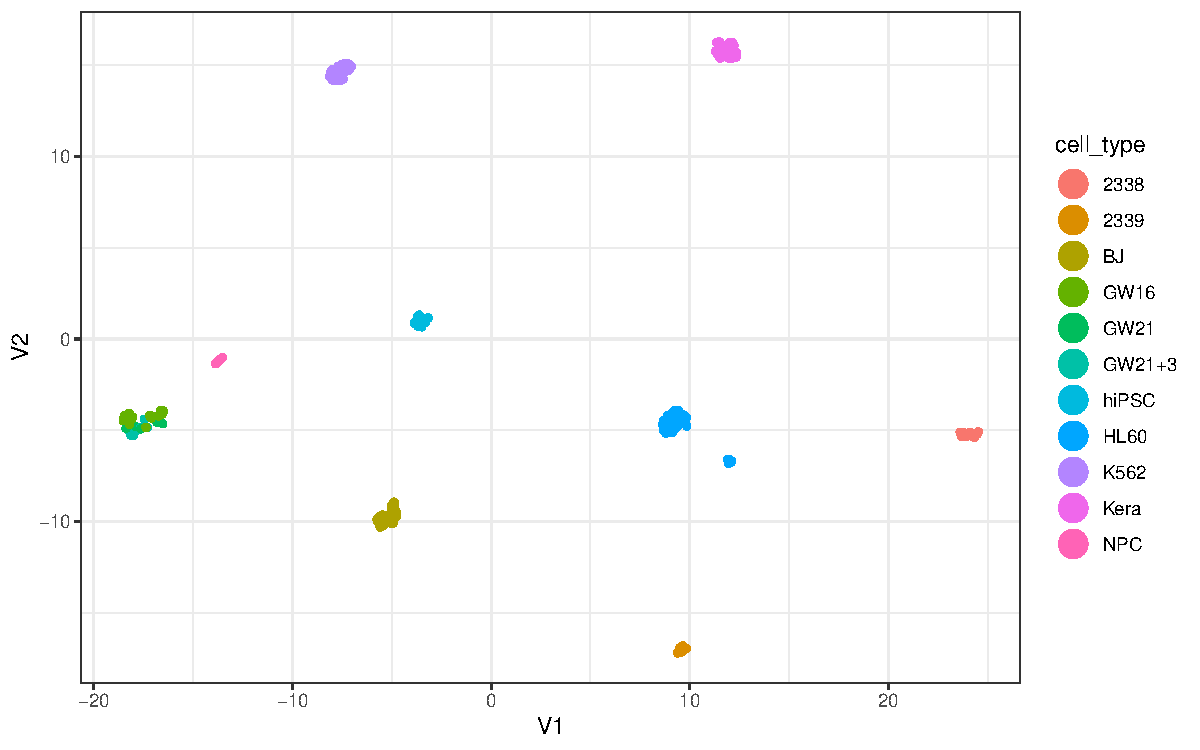
\includegraphics[width=\textwidth]{figures/plot-1} 
\end{knitrout}

\end{frame}


\begin{frame}
  \frametitle{To conclude}
  
  \begin{center}
      You can play online on \href{https://projector.tensorflow.org/}{https://projector.tensorflow.org/}
  \end{center}
  
\end{frame}

\end{document}

